% ===========================================================================
%  纵列双发矢量推力飞行器固件 EKF 组合导航：理论与算法分析设计报告
%  主入口文件
% ===========================================================================
% ===========================================================================
%  固件 EKF 组合导航理论与算法分析设计报告 —— 公共导言区
% ===========================================================================
\documentclass[UTF8,a4paper,12pt]{ctexart}

% ---------- 页面与段落 ----------
\usepackage[top=2.6cm,bottom=2.6cm,left=2.7cm,right=2.5cm]{geometry}
\usepackage{setspace}
\onehalfspacing
\setlength{\parindent}{2em}
\setlength{\parskip}{0.2em}
\setlength{\emergencystretch}{2em}
\raggedbottom
\clubpenalty=10000
\widowpenalty=10000
\displaywidowpenalty=10000
\usepackage{microtype}

% ---------- 页眉页脚与标题层级 ----------
\usepackage{fancyhdr}
\usepackage{titlesec}
\usepackage{caption}
\setcounter{tocdepth}{2}
\setcounter{secnumdepth}{3}
\setlength{\headheight}{15pt}
\pagestyle{fancy}
\fancyhf{}
\fancyhead[L]{\small\kaishu 纵列双发矢量推力飞行器固件 EKF 组合导航}
\fancyhead[R]{\small\kaishu 理论与算法分析设计报告}
\fancyfoot[C]{\small\thepage}
\renewcommand{\headrulewidth}{0.35pt}
\renewcommand{\footrulewidth}{0pt}
\fancypagestyle{plain}{%
  \fancyhf{}
  \fancyfoot[C]{\small\thepage}
  \renewcommand{\headrulewidth}{0pt}
  \renewcommand{\footrulewidth}{0pt}
}
\titleformat{\section}{\Large\bfseries}{\thesection}{0.8em}{}
\titleformat{\subsection}{\large\bfseries}{\thesubsection}{0.8em}{}
\titleformat{\subsubsection}{\normalsize\bfseries}{\thesubsubsection}{0.8em}{}
\titlespacing*{\section}{0pt}{2.0ex plus .5ex minus .2ex}{1.0ex}
\titlespacing*{\subsection}{0pt}{1.5ex plus .4ex minus .2ex}{0.7ex}
\titlespacing*{\subsubsection}{0pt}{1.2ex plus .3ex minus .2ex}{0.5ex}

% ---------- 数学与定理 ----------
\usepackage{amsmath,amssymb,amsthm}
\usepackage{mathtools}
\usepackage{bm}
\usepackage{bbm}
\theoremstyle{definition}
\newtheorem{definition}{定义}[section]
\theoremstyle{plain}
\newtheorem{theorem}{定理}[section]
\theoremstyle{remark}
\newtheorem{remark}{备注}[section]
\newtheorem*{notation}{符号约定}

% ---------- 图表 ----------
\usepackage{graphicx}
\usepackage{float}
\usepackage{placeins}
\usepackage{tikz}
\usepackage{pgfplots}
\pgfplotsset{compat=1.18}
\usepgfplotslibrary{groupplots}
\usetikzlibrary{arrows.meta,shapes,positioning,calc,patterns,angles,quotes,3d,backgrounds,fit}
\usepackage{booktabs}
\usepackage{array}
\usepackage{tabularx}
\usepackage{multirow}
\captionsetup{font=small,labelfont=bf,labelsep=space,justification=centering}

% ---------- 代码 ----------
\usepackage{listings}
\lstset{
  basicstyle=\ttfamily\small,
  frame=single,
  numbers=left,
  numberstyle=\tiny\color{gray},
  breaklines=true,
  columns=flexible,
  keepspaces=true,
  language=C++,
  commentstyle=\color{teal},
  keywordstyle=\color{blue},
}

% ---------- 引用与链接 ----------
\usepackage[numbers,sort&compress]{natbib}
\bibliographystyle{gbt7714-numeric}
\usepackage[hidelinks,unicode]{hyperref}
\usepackage{cleveref}
\hypersetup{
  pdftitle={纵列双发矢量推力飞行器固件 EKF 组合导航：理论与算法分析设计报告},
  pdfauthor={LShang},
  pdfsubject={15 状态误差状态 EKF 组合导航的理论推导、算法设计与仿真验证},
  pdfkeywords={EKF, 捷联惯导, GNSS 组合导航, 双子样圆锥补偿, 静止辅助, 误差状态}
}
\crefname{equation}{式}{式}
\crefname{figure}{图}{图}
\crefname{table}{表}{表}
\crefname{section}{节}{节}
\crefname{subsection}{节}{节}
\crefname{subsubsection}{节}{节}
\crefname{appendix}{附录}{附录}
\renewcommand{\refname}{参考文献}

% ---------- 列表 ----------
\usepackage{enumitem}
\setlist{nosep,leftmargin=2.2em}

% ---------- 自定义命令 ----------
% 常用矩阵/矢量记号
\newcommand{\vp}[1]{\boldsymbol{#1}}          % 粗体矢量
\newcommand{\m}[1]{\boldsymbol{#1}}            % 粗体矩阵
\newcommand{\q}[1]{\mathfrak{#1}}              % 四元数
% 注意：\dtheta / \dphi 本身已是粗体符号；\sk{} 直接括起已加粗参数，不再二次加粗
\newcommand{\dtheta}{\boldsymbol{\theta}}
\newcommand{\dphi}{\boldsymbol{\phi}}
\newcommand{\dx}{\delta\vp{x}}
\newcommand{\Cbn}{\m{C}_b^n}
\newcommand{\Cnb}{\m{C}_n^b}
\newcommand{\I}[1]{\m{I}_{#1}}
\newcommand{\E}[1]{\mathbb{E}\left[#1\right]}
\newcommand{\diag}{\operatorname{diag}}
\newcommand{\sk}[1]{[\,#1\,\times]}
\newcommand{\tr}{\operatorname{tr}}
\newcommand{\T}{^{\top}}
\newcommand{\inv}{^{-1}}
\newcommand{\Exp}{\operatorname{Exp}}
\newcommand{\Log}{\operatorname{Log}}
\newcommand{\atan}[1]{\operatorname{atan}(#1)}
\newcommand{\atanh}[1]{\operatorname{atanh}(#1)}
\newcommand{\atanhtwo}{\operatorname{atan2}}
\newcommand{\cross}{\times}
\newcommand{\code}[1]{\texttt{#1}}

% 文件引用
\newcommand{\file}[1]{\textcolor{blue}{\texttt{#1}}}

% 表格列宽工具
\newcolumntype{L}[1]{>{\raggedright\arraybackslash}p{#1}}
\newcolumntype{C}[1]{>{\centering\arraybackslash}p{#1}}
\newcolumntype{R}[1]{>{\raggedleft\arraybackslash}p{#1}}

\usepackage{makecell}
\renewcommand{\theadfont}{\small\bfseries}


\title{\textbf{纵列双发矢量推力飞行器固件 EKF 组合导航：\\理论与算法分析设计报告}}
\author{LShang}
\date{2026年8月}

\begin{document}

\begin{titlepage}
\centering
{\zihao{1}\bfseries 纵列双发矢量推力飞行器固件\par}
\vspace{0.4em}
{\zihao{1}\bfseries EKF 组合导航\par}
\vspace{1.0em}
{\zihao{2}\bfseries 理论与算法分析设计报告\par}
\vspace{1.6em}
{\Large Theory and Algorithm Analysis \& Design Report of the\par}
\vspace{0.3em}
{\Large Onboard EKF Integrated Navigation System\par}
\vspace{2.2em}
{\large LShang\par}
\vspace{0.5em}
{\large 2026年8月\par}

\vfill
\begin{minipage}{0.94\textwidth}
\textbf{摘要：}
本报告对纵列双发矢量推力飞行器飞控固件中的 EKF 组合导航系统进行系统的理论与
算法分析。该系统以 15 状态误差状态扩展卡尔曼滤波器为核心，融合 IMU 捷联惯导
解算、GNSS 位置/速度量测以及静止辅助量测（零速修正、重力方向、静止陀螺零偏、
姿态与航向量测），并辅以独立运行的垂直/水平卡尔曼滤波器与双矢量航向融合。
报告沿``坐标系与随机过程基础 $\rightarrow$ 地球模型 $\rightarrow$ 捷联编排
$\rightarrow$ 误差状态线性化 $\rightarrow$ 量测模型 $\rightarrow$ 鲁棒性机制
$\rightarrow$ 任务集成''的技术主线，逐项给出与固件源码逐行对照的公式推导、
算法设计与实现分析，包括双子样圆锥/划摇补偿、GNSS 延迟回放重传播、NIS 门控、
失联协方差膨胀与低增益重捕获、动态 GNSS 噪声加权等工程化机制的数学模型。
报告最后基于固件真实参数构建独立数值仿真，设计六个场景（静基座零偏收敛、
GNSS 融合、失联重捕获、延迟回放、双矢量航向、NIS 野值门控），验证滤波器行为
并给出定量分析，其中静基座水平加速度零偏的可观性限制、失联期位置漂移增长
等结论直接指导固件参数设计与使用边界。

\vspace{0.6em}
\noindent\textbf{关键词：}误差状态 EKF；捷联惯导；GNSS 组合导航；双子样圆锥补偿；
静止辅助；NIS 门控；GNSS 延迟回放

\vspace{1.4em}
\textbf{Abstract:}
This report presents a systematic theoretical and algorithmic analysis of the
EKF integrated navigation system in the flight-control firmware of a tandem
twin-engine vector-thrust aircraft. The system is built around a 15-state
error-state extended Kalman filter that fuses strapdown inertial navigation,
GNSS position/velocity measurements, and static-aid measurements (zero-velocity
update, gravity direction, static gyro bias, attitude and heading), supported by
independently running vertical/horizontal Kalman filters and dual-vector heading
fusion. Along the technical thread of \emph{coordinate systems and stochastic
models} $\rightarrow$ \emph{earth model} $\rightarrow$ \emph{strapdown
mechanization} $\rightarrow$ \emph{error-state linearization} $\rightarrow$
\emph{measurement models} $\rightarrow$ \emph{robustness mechanisms}
$\rightarrow$ \emph{task integration}, the report provides line-by-line
code-correlated derivations, algorithm design, and implementation analysis,
covering two-sample coning/sculling compensation, GNSS delay replay with
re-propagation, NIS gating, outage covariance inflation with low-gain
re-acquisition, and dynamic GNSS noise weighting. An independent numerical
simulation with firmware-real parameters is developed, and six scenarios are
designed to validate filter behavior quantitatively, including observability
limits of the horizontal accelerometer bias during pure static conditions and
position drift growth during GNSS outage.

\vspace{0.6em}
\noindent\textbf{Keywords:} error-state EKF; strapdown inertial navigation;
GNSS/INS integration; two-sample coning compensation; static aiding; NIS
gating; GNSS delay replay
\end{minipage}
\end{titlepage}

\clearpage
\pagenumbering{roman}
\tableofcontents
\thispagestyle{plain}

\clearpage
\pagenumbering{arabic}

% ===========================================================================
%  正文
% ===========================================================================
% ===========================================================================
%  第 1 章 引言
% ===========================================================================
\section{引言}

\subsection{背景与动机}

纵列双发矢量推力飞行器（tandem twin-engine vector-thrust aircraft）是一类以
纵列布置的双电机、正交单轴摆座与反向旋转螺旋桨为主要执行机构的垂直起降
（VTOL）概念飞行器。其飞控固件在 2026 年 8 月已完成实机首飞验证并进入调参优化
阶段，姿态控制、执行器分配、遥测链路等子系统均已形成稳定代码基线。在这些子系统
之上，状态估计——尤其是组合导航系统——承担着向控制律提供连续、一致、可用的姿态、
速度与位置信号的职责，是闭环控制、定高/定点模式以及 GNSS 丢失后安全退化共同依赖
的基础设施。

固件中的组合导航系统并非单一滤波器，而是一组按``精度层级''与``任务优先级''
组织的多级状态估计架构：
\begin{itemize}
  \item \textbf{主滤波器}：15 状态误差状态扩展卡尔曼滤波器（Ekf15State），
    状态包括 NED 位置误差、NED 速度误差、体系姿态误差、加速度计零偏误差与陀螺
    零偏误差，以 200\,Hz 的 IMU 捷联惯导解算为时间更新，以 GNSS 位置/速度量测及
    多类辅助量测为量测更新；
  \item \textbf{独立垂直滤波器}：2 状态（高度+速度）卡尔曼滤波器，融合 IMU 垂直
    加速度与气压计/激光测距高度，为垂直控制通道提供与主滤波器相互独立的冗余估计；
  \item \textbf{独立水平滤波器}：北/东两轴各 2 状态的卡尔曼滤波器，融合 IMU 水平
    加速度与光流速度，为无 GNSS 环境下的水平定位提供备份；
  \item \textbf{双矢量航向融合}：利用 GPS 地速矢量与光流机体速度矢量几何解算真实
    航向，作为主滤波器的标量航向量测，抑制陀螺积分航向漂移；
  \item \textbf{辅助逻辑}：统一静止检测器、静止辅助强度分级调度、GNSS 动态权重、
    GNSS 历元时间映射、气压高度基准换算等平台无关纯函数模块。
\end{itemize}

这套架构在工程上体现了``单一高精度主滤波器 + 分层冗余备份 + 防御性门控''的设计
思想：主滤波器保证 GNSS 可用时的最优融合精度；独立滤波器与备用 AHRS 保证 GNSS
丢失时的可用性；NIS 门控、物理残差门限、协方差稳定化与输入合法性防御则保证在
传感器异常、野值、信号失锁等恶劣条件下的数值安全。

本报告的目的，是对这套组合导航系统进行逐层、逐式、逐行的理论与算法分析：
把固件代码中的每一个矩阵块、每一处增益调度、每一组门限常量，还原为严格的数学
推导与明确的物理语义，并基于固件真实参数构建独立数值仿真对其行为进行定量验证。
该工作服务于三个层面的需求：
\begin{enumerate}
  \item \textbf{设计与评审}：为固件参数调优、后续扩展（如 RTK、视觉、气压计零偏
    状态化）提供经得起推敲的数学模型基础；
  \item \textbf{教学与传承}：使 3968 行的滤波器核心代码不再依赖``注释即文档''，
    而具备可与公式一一对照的完整理论映射；
  \item \textbf{验证与审计}：通过独立仿真复现滤波器在典型场景下的行为，检验算法
    语义与实现的一致性，并明确系统的适用边界。
\end{enumerate}

\subsection{分析对象与代码范围}

本报告的分析对象为固件源码目录 \file{TandemVec\_FCS} 下的导航相关文件，
\cref{tab:code-scope} 列出全部被分析文件及其角色。其中 \file{ekf\_15\_state.h}
是滤波器核心（约 3968 行），本报告对其内部数学实现进行逐段还原；\file{navigation\_task.cpp}
是 200\,Hz 导航任务主循环（约 1769 行），本报告对其状态机、辅助调度与输出桥接
进行流程级分析；其余 \file{include/} 下的 \code{ins\_*}.h 系列为平台无关纯函数
模块，可独立编译与宿主测试，本报告对其算法语义逐一给出数学描述。

\begin{table}[H]
\centering
\caption{本报告分析固件代码范围一览}
\label{tab:code-scope}
\small
\begin{tabularx}{\textwidth}{@{}L{5.2cm}L{2.6cm}X@{}}
\toprule
\textbf{文件} & \textbf{规模} & \textbf{角色} \\
\midrule
\file{lib/navigation-main/src/ekf\_15\_state.h} & 3968 行 & 15 状态误差状态 EKF 核心：
  初始化对准、单/双子样时间更新、协方差传播与稳定化、GNSS/速度/重力/姿态/航向/
  静止陀螺/气压高度量测更新、GNSS 延迟回放重传播 \\
\file{src/navigation\_task.cpp} & 1769 行 & 200\,Hz 导航任务：IMU 降采样与双子样
  组装、静止检测调度、GNSS 历元队列消费与质量检查、辅助量测调度、输出桥接、垂直
  速度多源估计、垂直/水平 KF 任务 \\
\file{include/VerticalKF\_2State.h} & 311 行 & 2 状态垂直 KF（高度+速度）\\
\file{include/HorizontalKF.h} & 245 行 & 单轴 2 状态水平 KF（位置+速度，光流速度观测）\\
\file{include/ins\_gnss\_dynamic\_weight.h} & 125 行 & GNSS 动态权重 R（clamp + pDOP 缩放）\\
\file{include/ins\_gnss\_epoch\_timing.h} & 94 行 & GNSS iTOW$\rightarrow$本地时刻映射与量测年龄 \\
\file{include/ins\_static\_detector.h} & 259 行 & 静止检测器（阈值+迟滞+置信度）\\
\file{include/ins\_static\_aid\_profile.h} & 161 行 & 静止辅助强度分级调度 \\
\file{include/ins\_altitude\_reference.h} & 37 行 & 气压高度基准换算 \\
\bottomrule
\end{tabularx}
\end{table}

\subsection{相关工作与技术背景}

组合导航（INS/GNSS 融合）经过数十年发展已形成成熟的理论体系，本报告的分析
建立在以下经典工作的基础之上：

\begin{itemize}
  \item \textbf{捷联惯导编排}：Savage \cite{Savage1998,Savage1998b} 系统地
    建立了捷联惯导算法的统一框架，包括圆锥/划摇补偿的通用形式与误差分析；
    Titterton \& Weston \cite{Titterton2014} 给出工程导向的完整教材性推导；
  \item \textbf{INS/GNSS 融合架构}：Groves \cite{Groves2013} 对松耦合、
    紧耦合与深耦合架构、误差状态滤波、量测建模进行了全面论述；Farrell \&
    Barth \cite{Farrell2000} 侧重 GPS 与惯导融合的实践细节；
  \item \textbf{误差状态四元数滤波}：Sol{\`a} \cite{Sola2017} 给出了
    ES-EKF 中四元数误差状态、指数映射与误差传播的现代系统化表述，与固件
    ``体系右乘误差角''的选取一致；Markley \cite{Markley1999} 分析了不同
    姿态误差表示对滤波性能的影响；
  \item \textbf{姿态滤波与互补滤波}：Madgwick \cite{Madgwick2011} 与 Mahony
    \cite{Mahony2008} 的梯度下降/互补滤波器被固件用作备用 AHRS（\code{backup\_ahrs}）
    与无 GNSS 时的姿态量测源；
  \item \textbf{随机过程与估计理论}：Maybeck \cite{Maybeck1979} 给出随机过程
    模型（高斯-马尔可夫）与卡尔曼滤波的经典论述；Crassidis \& Junkins
    \cite{crassidis2011} 覆盖可观测性（Gramian）与最优估计的理论工具；
  \item \textbf{大地参考}：WGS-84 椭球定义与 Somigliana 重力模型
    \cite{NAVSTAR2000} 是地球模型部分的权威依据。
\end{itemize}

本报告在以上理论框架下，以固件源码为``规范实现''，将每一项通用理论还原为
该特定实现的具体形式（含数值常量、调度策略与门限），形成一份可逐行对照的
工程分析文档。

\subsection{报告组织结构}

本报告沿``从物理到实现、从推导到验证''的递进结构组织，共 11 章：

\begin{itemize}
  \item \textbf{第 2 章（数学基础）}：定义坐标系、四元数与旋转矢量、斜对称算子、
    高斯-马尔可夫随机过程、离散化与线性化等全篇共用的数学工具，并给出误差状态
    卡尔曼滤波的一般框架；
  \item \textbf{第 3 章（地球模型）}：推导 WGS-84 椭球几何（子午圈/卯酉圈曲率
    半径）、Somigliana 正常重力模型、地球自转与传输速率、经纬高（LLA）运动学，
    并逐项对照固件 \file{earth\_model.h} 与 \file{ekf\_15\_state.h} 中的实现；
  \item \textbf{第 4 章（捷联惯导编排）}：推导姿态/速度/位置的离散递推，重点展开
    双子样圆锥补偿与划摇补偿的数学模型、中点重力与科氏力补偿、导航系转动补偿，
    以及固件中单/双子样路径的等价关系；
  \item \textbf{第 5 章（15 状态误差状态 EKF）}：建立 15 维误差状态、连续时间
    系统矩阵 $\m{F}$ 的完整推导（含完整 $\m{F}$ 矩阵扩展项）、协方差传播
    （一阶/二阶 $\bm{\Phi}$ 与 Simpson 离散过程噪声）、Joseph 协方差更新、
    误差状态注入与协方差稳定化；
  \item \textbf{第 6 章（量测模型）}：推导 GNSS 位置/速度量测（含
    LLA$\rightarrow$NED 新息）、速度量测、重力方向量测、姿态量测、标量航向量测、
    静止陀螺量测与气压高度量测的观测矩阵与观测噪声模型，并对每一处与固件实现
    对照；
  \item \textbf{第 7 章（静止辅助与调度）}：推导统一静止检测器的阈值、迟滞状态机
    与置信度评分，静止辅助三档强度调度（ZUPT/Gravity/StaticGyro）的降频策略及其
    可观性依据；
  \item \textbf{第 8 章（鲁棒性机制）}：分析 NIS 门控、物理残差门限、GNSS 失联
    协方差膨胀、低增益重捕获、GNSS 延迟回放重传播、输入合法性防御与协方差数值
    稳定化（Gershgorin/LDLT/特征值投影）的数学模型与设计权衡；
  \item \textbf{第 9 章（任务集成）}：给出 200\,Hz 导航任务的状态机、GNSS 历元
    队列消费、动态权重配置、重锚定逻辑、输出桥接（EKF/备用 AHRS/DETA100 三路
    切换）以及独立垂直/水平滤波器的任务分工；
  \item \textbf{第 10 章（仿真验证）}：基于固件真实参数构建独立数值仿真，设计六个
    场景并给出图表化结果与定量分析；
  \item \textbf{第 11 章（结论）}：总结全篇结论、固件设计特点与后续工作建议。
\end{itemize}

\subsection{主要结论预览}

本报告在分析中形成以下关键结论，正文将给出完整推导与证据：
\begin{enumerate}
  \item 固件采用\textbf{体系右乘误差角} $\delta\vp{\beta}^b$（
    $q = q_{nom}\otimes\Exp(\delta\vp{\beta}^b)$）的姿态误差定义，由此
    $\m{F}_{\Phi V}$ 块带 $\m{C}_n^b$ 旋转项（固件第 2397--2401 行），与
    导航系左乘误差的 KF-GINS 差一个旋转，实为同构；
  \item 协方差传播使用\textbf{双精度 Simpson 离散过程噪声}
    $Q_d = \frac{dt}{6}\left(Q_c + 4\Phi_{\frac12}Q_c\Phi_{\frac12}\T +
    \Phi Q_c\Phi\T\right)$（固件第 2592--2596 行），在 15$\times$15 规模下
    兼顾精度与嵌入式开销；
  \item 静止辅助的量测噪声与频率按置信度\textbf{分三档递减}，其核心依据是
    速度/重力方向量测对陀螺零偏的弱可观性——需要足够长的静止驻留与适当的量测
    频率配合才能收敛；
  \item GNSS 失联后位置协方差按经验增长率膨胀（水平 1.2\,m/s、垂直 1.8\,m/s），
    重捕获时对物理残差合理的量测采用\textbf{膨胀 R 低增益融合}，避免单帧跳变
    （固件第 1620--1644 行）；
  \item GNSS 延迟回放（15\,ms 历史缓冲重传播）将延迟量测严格对齐到其观测历元，
    消除``当前时刻直接融合''引入的时间失配误差。
\end{enumerate}

% ===========================================================================
%  第 2 章 数学基础
% ===========================================================================
\section{数学基础}

本章建立全篇共用的数学工具与记号约定，包括坐标系、姿态参数化、矢量代数算子、
随机过程模型、非线性系统离散化与线性化，以及误差状态卡尔曼滤波的一般框架。
后续各章直接引用本章定义而不重复推导。

\subsection{坐标系约定}

本报告与固件采用完全一致的坐标系约定，可归纳为三个层次：
\begin{enumerate}
  \item \textbf{导航系 NED}（North-East-Down，记为 $n$ 系）：以起飞点为原点
    （或地心地固系投影点），$x$ 轴指向北、$y$ 轴指向东、$z$ 轴指向地心方向
    （向下为正），构成右手正交系；
  \item \textbf{机体系 FRD}（Front-Right-Down，记为 $b$ 系）：固连于机体，
    $x$ 轴指向前方、$y$ 轴指向右翼、$z$ 轴指向机腹（向下为正），右手正交系；
  \item \textbf{地心惯性系} 与 \textbf{地心地固系（ECEF）}：用于地球自转与
    WGS-84 椭球几何，第 3 章给出其与本报告直接相关的投影关系。
\end{enumerate}

\begin{definition}[方向余弦矩阵]
设 $\vp{r}^n \in \mathbb{R}^3$ 为导航系坐标，$\vp{r}^b \in \mathbb{R}^3$ 为
机体系坐标，则
\begin{equation}
  \vp{r}^n = \m{C}_b^n\, \vp{r}^b, \qquad
  \vp{r}^b = \m{C}_n^b\, \vp{r}^n,
  \label{eq:dcm-def}
\end{equation}
其中 $\m{C}_b^n = (\m{C}_n^b)\T$ 为正交旋转矩阵（$\det = +1$）。固件中以
\code{t\_b2ned} 缓存 $\m{C}_b^n$（见 \file{ekf\_15\_state.h} 第 3912 行注释）。
\end{definition}

需要特别说明 NED 系中``地''（Down）分量与习惯``高度''的关系：若 $h$ 为 WGS-84
椭球高（向上为正），则 NED 位置误差第三分量 $\delta p_D = -\delta h$。这一符号
约定贯穿第 5 章误差状态与第 6 章量测模型的全部分析，与固件注释
``NED的D向下为正，D误差增大等价高度降低''（\file{ekf\_15\_state.h} 第 2320 行）
一致。

\subsection{四元数与旋转矢量}

\subsubsection{四元数代数}

\begin{definition}[单位四元数]
单位四元数
\begin{equation}
  q = \begin{bmatrix} q_w \\ \vp{q}_v \end{bmatrix}
    \in \mathbb{H},\qquad \|q\|^2 = q_w^2 + \vp{q}_v^\top \vp{q}_v = 1
  \label{eq:quat-def}
\end{equation}
参数化从机体系到导航系的旋转，其与轴角 $\left(\vp{u},\,\phi\right)$ 的关系为
$q_w = \cos(\phi/2)$，$\vp{q}_v = \vp{u}\sin(\phi/2)$。
\end{definition}

四元数乘法（Hamilton 积）定义为
\begin{equation}
  q \otimes p =
  \begin{bmatrix}
    q_w p_w - \vp{q}_v^\top\vp{p}_v \\
    q_w \vp{p}_v + p_w \vp{q}_v + \vp{q}_v \cross \vp{p}_v
  \end{bmatrix},
  \label{eq:quat-prod}
\end{equation}
其对应旋转的合成次序为 $R(q\otimes p) = R(q)\,R(p)$。共轭为
$q^{*} = \begin{bmatrix} q_w & -\vp{q}_v^\top \end{bmatrix}\T$。固件使用
\code{Eigen::Quaternionf} 存储，分量顺序为 (w,x,y,z)（见
\file{ekf\_15\_state.h} 第 1448--1467 行）。

\subsubsection{旋转矢量与指数映射}

\begin{definition}[旋转矢量]
旋转矢量 $\dtheta = \vp{u}\,\phi \in \mathbb{R}^3$ 以轴角形式描述一次旋转：
方向为旋转轴、模长为旋转角。由旋转矢量到四元数的\textbf{指数映射}为
\begin{equation}
  q = \Exp(\dtheta) =
  \begin{bmatrix}
    \cos\left(\tfrac{\|\dtheta\|}{2}\right) \\
    \vp{u}\sin\left(\tfrac{\|\dtheta\|}{2}\right)
  \end{bmatrix},
  \qquad \vp{u} = \dtheta / \|\dtheta\|.
  \label{eq:exp-map}
\end{equation}
其逆映射（对数映射）为
\begin{equation}
  \dtheta = \Log(q) = 2\,\arccos(q_w)\,\frac{\vp{q}_v}{\|\vp{q}_v\|},
  \label{eq:log-map}
\end{equation}
当 $\|\vp{q}_v\|$ 极小（$<10^{-6}$）时固件退化为一阶近似
$\Log(q) \approx 2\vp{q}_v$（\file{ekf\_15\_state.h} 第 1778--1801 行
\code{BuildDeltaQuatFromRotationVector}）。
\end{definition}

指数映射在误差状态滤波中承担两个关键角色：一是 IMU 角增量对四元数的推进
（第 4 章），二是姿态误差状态向全量姿态的注入（第 5 章第 5.5 节）。用指数映射
而非小角度一阶近似，可在单次大修正（如 AHRS 量测给出 $0.5$\,rad 级误差）时避免
修正量被低估。

\subsubsection{旋转的小角度一阶展开}

设 $\m{R} \in SO(3)$，微旋转 $\Exp(\dtheta)$ 作用于 $\m{R}$ 右侧，则
\begin{equation}
  \m{R}\,\Exp(\dtheta) \approx \m{R}\left(\m{I}_3 + \sk{\dtheta}\right)
  = \m{R} + \m{R}\,\sk{\dtheta},
  \label{eq:small-rotation}
\end{equation}
其中 $\sk{\cdot}$ 为斜对称算子（见第 2.3 节）。对任意矢量 $\vp{v}$，
\begin{equation}
  \m{R}\sk{\dtheta}\vp{v}
  = \m{R}(\dtheta \cross \vp{v})
  = (\m{R}\dtheta) \cross (\m{R}\vp{v})
  = \sk{\m{R}\dtheta}\,\m{R}\vp{v},
  \label{eq:skew-rot-commute}
\end{equation}
由此得到斜对称算子与旋转矩阵的交换律
\begin{equation}
  \m{R}\,\sk{\dtheta}\,\m{R}^\top = \sk{\m{R}\dtheta}.
  \label{eq:skew-rot}
\end{equation}
\cref{eq:skew-rot} 是第 6 章重力方向量测观测矩阵推导（
$H_{att} = \sk{\m{C}_b^n\,\vp{g}_{sf}^n}$）的核心工具。

\subsection{斜对称算子}

\begin{definition}[斜对称算子]
对任意 $\vp{v} = \begin{bmatrix} v_1 & v_2 & v_3 \end{bmatrix}\T$，
\begin{equation}
  \sk{\vp{v}} \triangleq
  \begin{bmatrix}
    0 & -v_3 & v_2 \\
    v_3 & 0 & -v_1 \\
    -v_2 & v_1 & 0
  \end{bmatrix},
  \qquad
  \sk{\vp{v}}\,\vp{w} = \vp{v} \cross \vp{w}.
  \label{eq:skew-def}
\end{equation}
其性质包括：$\sk{\vp{v}}\T = -\sk{\vp{v}}$；$\sk{\alpha\vp{v} + \beta\vp{w}}
= \alpha\sk{\vp{v}} + \beta\sk{\vp{w}}$（线性）；以及 Jacobi 恒等式
$\sk{\vp{v}}\sk{\vp{w}} - \sk{\vp{w}}\sk{\vp{v}}
= \sk{\sk{\vp{v}}\vp{w}}$。
\end{definition}

\subsection{随机过程模型}

\subsubsection{高斯白噪声与谱密度}

本报告采用连续时间高斯白噪声模型描述 IMU 与量测传感器的随机误差。设
$\vp{w}(t)$ 为零均值白噪声，其功率谱密度（PSD）为 $\m{Q}_c$，则
\begin{equation}
  \E{\vp{w}(t)\vp{w}(t')\T} = \m{Q}_c\,\delta(t - t'),
  \label{eq:white-noise}
\end{equation}
其中 $\delta(\cdot)$ 为 Dirac 函数。白噪声通过线性时不变系统
$\dot{\vp{x}} = \m{A}\vp{x} + \m{G}\vp{w}$ 后，其稳态协方差
$\m{P}_{\infty}$ 满足 Lyapunov 方程
\begin{equation}
  \m{A}\m{P}_{\infty} + \m{P}_{\infty}\m{A}\T + \m{G}\m{Q}_c\m{G}^\top = \m{0}.
  \label{eq:lyapunov}
\end{equation}

\subsubsection{一阶高斯-马尔可夫过程}

固件将加速度计与陀螺的零偏建模为一阶高斯-马尔可夫（Gauss-Markov）过程：
\begin{equation}
  \dot{\vp{b}}(t) = -\frac{1}{\tau}\,\vp{b}(t) + \vp{w}_b(t),
  \qquad
  \E{\vp{w}_b(t)\vp{w}_b(t')\T} = \m{Q}_b\,\delta(t-t'),
  \label{eq:gm-process}
\end{equation}
其中 $\tau$ 为相关时间常数。其稳态方差与驱动噪声谱密度满足
\begin{equation}
  \sigma_b^2 = \frac{\tau}{2}\,q_b,
  \qquad\text{即}\qquad
  q_b = \frac{2\sigma_b^2}{\tau},
  \label{eq:gm-variance}
\end{equation}
这正是固件初始化过程噪声矩阵时采用的形式
（\file{ekf\_15\_state.h} 第 523--530 行）：
\begin{equation}
  rw_{b} = \frac{2\,\sigma_{b}^2}{\tau}\,\m{I}_3,
  \label{eq:gm-rw}
\end{equation}
其中 $\sigma_b$ 对应固件的 \code{accel\_markov\_bias\_std\_mps2} 与
\code{gyro\_markov\_bias\_std\_radps}，$\tau$ 对应 \code{accel\_tau\_s}（100\,s）
与 \code{gyro\_tau\_s}（180\,s，固件运行配置）。

\begin{remark}
一阶高斯-马尔可夫过程在误差状态中体现为对角衰减块
$\m{F}_{b} = -\m{I}_3/\tau$（第 5 章第 5.3 节），其含义是零偏误差以时间常数
$\tau$ 向零回归，同时被驱动噪声持续激励。$\tau$ 越大，零偏变化越慢，长时稳定性
越好但短时修正越保守——固件将陀螺 $\tau$ 设为 180\,s 即取这一权衡
（\file{navigation\_task.cpp} 第 851 行）。
\end{remark}

\subsubsection{随机过程的离散化}

对一阶高斯-马尔可夫过程 \cref{eq:gm-process}，在采样间隔 $dt$ 内精确离散化为
\begin{equation}
  \vp{b}_k = e^{-dt/\tau}\,\vp{b}_{k-1} + \vp{w}_{d,k},
  \qquad
  \E{\vp{w}_{d,k}\vp{w}_{d,k}\T} = q_b\,\frac{\tau}{2}
    \left(1 - e^{-2dt/\tau}\right)\m{I}_3.
  \label{eq:gm-discrete}
\end{equation}
对误差状态滤波，零偏误差的离散递推由 $\bm{\Phi}$ 的零偏块
$\bm{\Phi}_{bb} = e^{-\m{I}_3 dt/\tau} \approx \left(1 - dt/\tau\right)\m{I}_3$
（二阶展开含 $\frac12(dt/\tau)^2$ 修正）与 $\m{Q}_d$ 的零偏块共同实现。
当 $dt \ll \tau$（固件 5\,ms vs.\ 100--180\,s）时，\cref{eq:gm-discrete} 的
驱动噪声方差近似为
\begin{equation}
  q_b\,\frac{\tau}{2}\left(1 - e^{-2dt/\tau}\right)
  \approx q_b\,dt\left(1 - \frac{dt}{\tau}\right)
  \approx \frac{2\sigma_b^2}{\tau}\,dt,
  \label{eq:gm-discrete-approx}
\end{equation}
即固件快速路径采用的对角注入形式 $\frac{2\sigma_b^2}{\tau}dt$（第 5.5.3 节）。

\subsubsection{IMU 误差参数的 Allan 方差对应}

MEMS IMU 数据手册以 Allan 方差给出随机误差参数，与本节谱密度的对应关系为
\cite{Groves2013,Titterton2014}：
\begin{itemize}
  \item \textbf{角度随机游走}（ARW）：陀螺白噪声 $\sigma_{gw}$ 对应的
    功率谱密度 $q_g = \sigma_{gw}^2$，Allan 方差在 $\tau=1$\,s 处取
    $ARW = \sigma_{gw}\,\text{rad}/\sqrt{\text{s}}$；
  \item \textbf{零偏不稳定性}（BI）：高斯-马尔可夫驱动噪声的稳态
    $BI = \sigma_B$，谱密度 $q_b = 2\sigma_B^2/\tau$（\cref{eq:gm-rw}）；
  \item \textbf{速率随机游走}（RRW）：陀螺零偏的长期漂移，在本模型中由
    高斯-马尔可夫过程的时间常数 $\tau_g$ 截断（纯积分随机游走是
    $\tau \to \infty$ 的极限情形）。
\end{itemize}
固件将陀螺零偏建模为 $\tau_g = 180$\,s 的一阶高斯-马尔可夫而非纯随机游走，
正是为了在长时间静止场景下让零偏误差保持有界，避免 P 矩阵因持续激励而过度
膨胀。

\subsubsection{卡方分布与 NIS 门限的统计推导}

设 $\vp{y} \sim \mathcal{N}(\m{0},\ \m{S})$（$\m{S}$ 正定），则二次型
\begin{equation}
  NIS = \vp{y}\T\m{S}\inv\vp{y} = \sum_{i=1}^{m} \left(\frac{y_i'}{\sigma_i}\right)^2
  \label{eq:nis-chi2}
\end{equation}
服从自由度为 $m$ 的中心卡方分布 $\chi^2_m$，其中 $y_i'$ 为白化后的独立
标准正态分量。其均值与方差为
\begin{equation}
  \E{NIS} = m, \qquad \operatorname{Var}(NIS) = 2m.
  \label{eq:nis-moments}
\end{equation}
对 $m$ 维量测，99\%/99.9\%/99.99\% 分位数（$\alpha = 0.01/0.001/0.0001$）
由正则化不完全伽马函数定义：
\begin{equation}
  P(\chi^2_m \le T) = \frac{\gamma(m/2,\ T/2)}{\Gamma(m/2)} = 1 - \alpha.
  \label{eq:chi2-quantile}
\end{equation}
固件各量测门限的选取（第 8.1 节 \cref{tab:nis-thresholds}）围绕 99.9\% 分位数
设计：GNSS（$m=6$）取 30（99.9\% $\approx22.5$，留机动容差）；重力/姿态
（$m=3$）取 18（99.9\% $\approx16.3$）；航向/气压（$m=1$）取 12/16（99.9\%
$\approx10.8$、99.99\% $\approx15.1$）。门限略高于统计值是为高动态机动下模型
线性化误差留裕量。

当滤波模型与实际噪声不一致时，$NIS$ 偏离 $\chi^2_m$：量测噪声被低估
（$\m{R}$ 过小）时 $NIS$ 偏大，易误拒；被高估时 $NIS$ 偏小，门控灵敏度下降。
第 10 章第 10.3 节通过正常帧 $NIS$ 均值（2.79）验证了固件配置的 $R$ 与仿真
噪声基本一致（略保守）。

\subsection{非线性系统离散化与线性化}

\subsubsection{系统模型}

考虑连续时间非线性系统与量测：
\begin{align}
  \dot{\vp{x}}(t) &= \vp{f}\big(\vp{x}(t),\,\vp{u}(t)\big) + \m{G}\vp{w}(t),
  \label{eq:cont-sys} \\
  \vp{z}_k &= \vp{h}(\vp{x}_k) + \vp{v}_k,
  \label{eq:meas-sys}
\end{align}
其中 $\vp{w}$、$\vp{v}$ 为零均值白噪声，协方差（PSD）分别为 $\m{Q}_c$、$\m{R}_k$，
互不相关。误差状态滤波器以标称轨迹 $\bar{\vp{x}}$ 线性化：
\begin{equation}
  \delta\dot{\vp{x}} \triangleq \dot{\vp{x}} - \dot{\bar{\vp{x}}}
  \approx \underbrace{\left.\frac{\partial \vp{f}}{\partial \vp{x}}\right|_{\bar{\vp{x}}}
  }_{\m{F}}\,\delta\vp{x} + \m{G}\vp{w}.
  \label{eq:error-sys}
\end{equation}

\subsubsection{状态转移矩阵离散化}

连续系统 \cref{eq:error-sys} 的离散化状态转移矩阵（STM）为矩阵指数：
\begin{equation}
  \bm{\Phi}(t_k,\,t_{k-1}) = e^{\m{F}\,dt}
  = \m{I}_n + \m{F}\,dt + \frac{1}{2}\m{F}^2\,dt^2 + \frac{1}{6}\m{F}^3\,dt^3 + \cdots
  \label{eq:matrix-exp}
\end{equation}
固件默认采用\textbf{二阶截断}
\begin{equation}
  \bm{\Phi} \approx \m{I}_{15} + \m{F}\,dt + \frac{1}{2}\,\m{F}^2\,dt^2,
  \label{eq:phi-second}
\end{equation}
并以编译宏 \code{BFS\_NAVIGATION\_EMBEDDED\_FAST\_FIRST\_ORDER\_PHI} 提供一阶
退化路径 $\bm{\Phi} \approx \m{I} + \m{F}\,dt$（\file{ekf\_15\_state.h} 第
2404--2426 行）。在 $dt = 5$\,ms、IMU 带宽以内的动态下，二阶截断误差为
$\mathcal{O}((\m{F}dt)^3)$，其中 $\|\m{F}\|\,dt \sim 10^{-3}$ 量级
（$\m{F}$ 的最大元素为角速度项 $\sim 10^0$\,rad/s），截断误差可以忽略。

\subsubsection{过程噪声离散化}

连续过程噪声 $\m{G}\m{Q}_c\m{G}^\top$ 需离散化为
\begin{equation}
  \m{Q}_d = \int_{t_{k-1}}^{t_k} \bm{\Phi}(t_k,\,s)\,\m{G}\m{Q}_c\m{G}^\top
  \bm{\Phi}(t_k,\,s)\T\,ds.
  \label{eq:qd-def}
\end{equation}
常见的零阶保持近似为 $\m{Q}_d \approx \m{G}\m{Q}_c\m{G}^\top dt$。固件采用更高精度的
\textbf{Simpson 积分}近似（\file{ekf\_15\_state.h} 第 2592--2596 行）：
\begin{equation}
  \m{Q}_d \approx \frac{dt}{6}\left(
    \m{Q}_c + 4\,\bm{\Phi}_{\frac12}\m{Q}_c\bm{\Phi}_{\frac12}^\top
    + \bm{\Phi}\m{Q}_c\bm{\Phi}^\top
  \right),
  \label{eq:simpson-qd}
\end{equation}
其中 $\bm{\Phi}_{\frac12} = \m{I} + \frac{dt}{2}\m{F} +
\frac12\left(\frac{dt}{2}\m{F}\right)^2$ 为半周期 STM。与一阶近似相比，
\cref{eq:simpson-qd} 对 $\m{F}$ 的耦合项（如速度误差块与姿态误差块之间的交叉）
保留了二阶以上的贡献，在强机动下避免过程噪声欠估计导致的滤波器过度自信。

\begin{remark}
当 $\m{G}$ 为恒定矩阵且 $\m{Q}_c$ 为块对角时，固件利用
$\m{C}_b^n\,\sigma^2\m{I}\,\m{C}_n^b = \sigma^2\m{I}$ 的正交不变性，将
$\m{G}\m{Q}_c\m{G}^\top$ 的稠密乘法化简为四个对角块直写
（\file{ekf\_15\_state.h} 第 2558--2578 行
\code{Icm45686StructuredContinuousQc}），在数学上与原式严格等价，仅省去稀疏
矩阵的无效乘法。
\end{remark}

\subsection{误差状态卡尔曼滤波}

\subsubsection{架构选择：误差状态 vs. 全状态}

本报告分析的对象——固件 \code{Ekf15State}——属于\textbf{误差状态扩展卡尔曼滤波}
（Error-State EKF, ES-EKF）\cite{Sola2017}。其思想是：将滤波状态拆分为
\begin{equation}
  \underbrace{\vp{x}_{full}}_{\text{全量状态}}
  = \underbrace{\bar{\vp{x}}}_{\text{标称/积分状态}}
  \oplus \underbrace{\dx}_{\text{误差状态}},
  \label{eq:state-split}
\end{equation}
其中标称状态由确定性动力学（捷联惯导编排）以高频率推进，误差状态则由线性化的
卡尔曼滤波估计并反馈注入。这一架构的优势在于：
\begin{itemize}
  \item \textbf{线性化点精确}：误差状态在零附近，一阶展开误差远小于全状态在
    大动态范围内线性化；
  \item \textbf{姿态误差维度紧凑}：姿态用 3 维旋转矢量而非 4 维四元数（带归一化
    约束），避免了四元数协方差的奇异性；
  \item \textbf{数值稳定}：误差状态量级小，协方差矩阵的条件数受控。
\end{itemize}

\subsubsection{标准递推}

设误差状态 $\dx \in \mathbb{R}^{n}$、协方差 $\m{P}$，则滤波递推为
\begin{align}
  \textbf{预测:}\quad
  \dx_{k|k-1} &= \bm{\Phi}_{k-1}\,\dx_{k-1|k-1}, &
  \m{P}_{k|k-1} &= \bm{\Phi}_{k-1}\m{P}_{k-1|k-1}\bm{\Phi}_{k-1}\T + \m{Q}_d,
  \label{eq:es-predict} \\
  \textbf{新息:}\quad
  \vp{y}_k &= \vp{z}_k - \vp{h}(\bar{\vp{x}}_{k|k-1}), &
  \m{S}_k &= \m{H}_k\m{P}_{k|k-1}\m{H}_k\T + \m{R}_k,
  \label{eq:es-innovation} \\
  \textbf{增益:}\quad
  \m{K}_k &= \m{P}_{k|k-1}\m{H}_k\T\m{S}_k\inv,
  \label{eq:es-gain} \\
  \textbf{更新:}\quad
  \dx_{k|k} &= \m{K}_k\vp{y}_k, &
  \m{P}_{k|k} &= \left(\m{I} - \m{K}_k\m{H}_k\right)\m{P}_{k|k-1}
    \left(\m{I} - \m{K}_k\m{H}_k\right)\T + \m{K}_k\m{R}_k\m{K}_k\T,
  \label{eq:es-update}
\end{align}
其中 \cref{eq:es-update} 的协方差更新采用\textbf{Joseph 形式}，保证数值上的
对称正定性。误差状态 $\dx_{k|k}$ 通过第 5.5 节的注入运算写回全量状态后清零。

\begin{remark}
Joseph 形式相对标准形式 $\m{P} = (\m{I}-\m{K}\m{H})\m{P}$ 增加约
$2n^2 m$ 次乘法，但在浮点运算中能够抵消舍入误差导致的负特征值，是嵌入式高维
滤波的工程惯例。固件在所有量测更新路径（GNSS/速度/重力/姿态/航向/气压高度）
中统一使用 Joseph 形式（见第 6 章各节），仅静止陀螺量测因只更新零偏子块而采用
子块化的等效形式（第 6.6 节）。
\end{remark}

% ===========================================================================
%  第 3 章 地球模型
% ===========================================================================
\section{地球模型与大地参考}

捷联惯导在地理坐标系（NED）中积分时，需要地球的几何与物理参数：曲率半径
（用于经纬高变化率）、正常重力（用于比力到线加速度的分解）、地球自转与导航系
转动（用于角速度补偿）。固件将地球模型集中封装在 \file{earth\_model.h} 与
\file{ekf\_15\_state.h} 的 \code{ComputeEarthModelTerms} /
\code{ComputeLlaRateGeometryTerms} 中，并采用 \code{double} 中间量以保证
绝对位置精度（\file{ekf\_15\_state.h} 第 3961 行注释说明 float32 在
$\sim113°$ 经度处约 0.75\,m 一跳）。本章给出这些模型的完整推导。

\subsection{WGS-84 椭球几何}

WGS-84 地球椭球以长半轴 $a_e = 6378137.0$\,m 与第一偏心率平方
$e^2 = 6.69437999014\times10^{-3}$ 定义。设纬度为 $\varphi$（弧度）、椭球高为
$h$，则椭球面上一点的\textbf{卯酉圈曲率半径}（prime vertical, 沿东西向）与
\textbf{子午圈曲率半径}（meridional, 沿南北向）为
\begin{align}
  R_N &= \frac{a_e}{\sqrt{1 - e^2\sin^2\varphi}},
  \label{eq:rn} \\
  R_M &= \frac{a_e\,(1 - e^2)}
    {\left(1 - e^2\sin^2\varphi\right)^{3/2}}.
  \label{eq:rm}
\end{align}
固件实现 \code{ComputeLlaRateGeometryTerms}（\file{ekf\_15\_state.h} 第
2047--2061 行）与 \code{ComputeEarthModelTerms}（第 2063--2103 行）均按
\cref{eq:rn}--\cref{eq:rm} 计算，并缓存 $\sin\varphi$、$\cos\varphi$、
$\tan\varphi$ 及平均半径
\begin{equation}
  R_{mean} = \sqrt{R_N R_M}.
  \label{eq:mean-radius}
\end{equation}

\cref{tab:wgs84} 汇总 WGS-84 椭球与重力参数及其在固件中的对应宏/常量。

\begin{table}[H]
\centering
\caption{WGS-84 椭球与地球物理参数（固件 \file{earth\_model.h} / \file{constants.h}）}
\label{tab:wgs84}
\small
\begin{tabularx}{\textwidth}{@{}L{5.4cm}C{3.4cm}C{3.4cm}X@{}}
\toprule
\textbf{参数} & \textbf{符号} & \textbf{数值} & \textbf{固件宏/常量} \\
\midrule
长半轴 & $a_e$ & 6378137.0 m & \code{SEMI\_MAJOR\_AXIS\_LENGTH\_M} \\
第一偏心率平方 & $e^2$ & $6.69437999014\times10^{-3}$ & \code{ECC2} \\
地球自转角速率 & $\omega_e$ & $7.2921151467\times10^{-5}$ rad/s & \code{WE\_RADPS} \\
赤道正常重力 & $\gamma_e$ & 9.780318 m/s² & \code{Somigliana} 系数 \\
椭球重力扁率项 & $\beta$ & $5.3024\times10^{-3}$ & \code{Somigliana} 系数 \\
重力二阶项 & $\beta_2$ & $-5.898\times10^{-6}$ & \code{Somigliana} 系数 \\
标准重力 & $g_0$ & 9.80665 m/s² & \code{G\_MPS2}（回退值）\\
\bottomrule
\end{tabularx}
\end{table}

\begin{remark}
纬度接近极点时 $\cos\varphi \to 0$，固件以 \code{MAX\_ABS\_ALT\_M=1e5} 与
\code{MIN\_COS\_LAT=1e-3} 限制输入范围（\file{ekf\_15\_state.h} 第
1689--1711 行），避免 $\tan\varphi$ 与 $1/\cos\varphi$ 溢出；运行期对
$\cos\varphi$ 再次做绝对值下界保护（第 2071--2074 行）。
\end{remark}

\subsection{重力异常的讨论}

\cref{eq:somigliana} 的 Somigliana 公式描述\textbf{正常重力}（参考椭球面
上的理论值），与实测重力（含大地水准面起伏、地壳密度异常）存在偏差——即
\textbf{重力异常}。对飞行器导航：
\begin{itemize}
  \item 重力异常的空间尺度在数十公里以上，幅度约 $10^{-3}$--$10^{-2}$\,m/s$^2$
    量级（山区更显著），其对短时飞行的姿态估计影响可忽略，但对长航时高精度
    惯导（如惯性导航系统连续数十分钟）会产生可积累的位置误差；
  \item 本飞行器为近地低速 VTOL（飞行范围 $<$公里级、航时 $<$30\,min），
    重力异常误差远小于 GNSS 观测噪声与 MEMS 零偏误差，正常重力模型
    \cref{eq:somigliana}--\cref{eq:gravity-alt} 已足够；
  \item 固件第 1352--1379 行对导出重力做低通滤波并限幅
    $[9.0,\ 10.5]$\,m/s$^2$，正是针对异常定位数据/重锚定瞬态的保护，而非
    重力异常本身。
\end{itemize}

\subsection{Somigliana 正常重力}

NED 系下的重力矢量沿地向（+D）。其模长随纬度与高度变化，固件采用
WGS-84/GRS-80 的 Somigliana 闭式：
\begin{equation}
  g_0(\varphi) = 9.780318\left(1 + 5.3024\times10^{-3}\,\sin^2\varphi
    - 5.898\times10^{-6}\,\sin^2 2\varphi\right),
  \label{eq:somigliana}
\end{equation}
再以\textbf{反平方形式}修正高度：
\begin{equation}
  g(h) = \frac{g_0}{\left(1 + h/R_{mean}\right)^2}.
  \label{eq:gravity-alt}
\end{equation}
\cref{eq:gravity-alt} 在 $h\ll R_{mean}$ 时展开为 $g \approx g_0(1 - 2h/R_{mean})$；
对 $h<0$（低于椭球面）必须采用 $(1+h/R)^{-2}$ 而非 $(1+h/R)$ 形式，否则符号错误。
固件在 \file{ekf\_15\_state.h} 第 2084--2097 行实现了 \cref{eq:somigliana}--
\cref{eq:gravity-alt}，并在注释中特别说明与 \file{earth\_model.h} 的
\code{normalgravity\_mps2()} 保持一致。纬度敏感性：$\partial g/\partial\varphi
\sim 5\times10^{-3}$\,m/s$^2$/度，故 \file{navigation\_task.cpp} 第 1364 行对
导出重力做 $\tau\approx1$\,s 低通滤波以抑制 LLA 噪声。

\subsection{地球自转与导航系转动}

\subsubsection{地球自转在 NED 系的投影}

地球自转角速率 $\omega_e = 7.2921151467\times10^{-5}$\,rad/s 在 NED 系
（$x$ 北、$y$ 东、$z$ 地）的投影为
\begin{equation}
  \vp{\omega}_{ie}^n = \begin{bmatrix}
    \omega_e\cos\varphi \\ 0 \\ -\omega_e\sin\varphi
  \end{bmatrix}.
  \label{eq:earth-rate-ned}
\end{equation}
固件 \code{ComputeEarthModelTerms} 第 2099--2101 行即按 \cref{eq:earth-rate-ned}
缓存 \code{earth\_rate\_ned\_radps}。

\subsubsection{导航系转动（传输速率）}

NED 导航系相对地球的转动角速率（transport rate）由速度与曲率半径决定：
\begin{equation}
  \vp{\omega}_{en}^n = \begin{bmatrix}
    \dfrac{v_E}{R_N + h} \\[1ex]
    -\dfrac{v_N}{R_M + h} \\[1ex]
    -\dfrac{v_E\tan\varphi}{R_N + h}
  \end{bmatrix}.
  \label{eq:nav-rate}
\end{equation}
固件 \code{ComputeNavRateFromTerms}（\file{ekf\_15\_state.h} 第 2131--2141 行）
按 \cref{eq:nav-rate} 实现。惯导解算中需要同时补偿两项：
\begin{itemize}
  \item \textbf{角速度补偿}：陀螺在机体系测得相对惯性系的角速度，减去导航系
    相对惯性系转动在机体系的投影后才是相对 NED 的姿态变化率：
    \begin{equation}
      \vp{\omega}_{nb}^b = \vp{\omega}_{ib}^b
        - \m{C}_n^b\left(\vp{\omega}_{ie}^n + \vp{\omega}_{en}^n\right);
      \label{eq:omega-nb}
    \end{equation}
  \item \textbf{科氏/向心加速度补偿}：比力方程中
    \begin{equation}
      \dot{\vp{v}}^n = \m{C}_b^n\vp{f}^b + \vp{g}^n
        - \left(2\vp{\omega}_{ie}^n + \vp{\omega}_{en}^n\right)\cross\vp{v}^n.
      \label{eq:coriolis}
    \end{equation}
\end{itemize}
固件 \code{PropagateStateFromIncrements} 中第 2269--2276 行分别实现
\cref{eq:omega-nb} 的导航系旋转增量（\code{nav\_frame\_delta\_theta\_rad}）与
\cref{eq:coriolis} 的科氏加速度（\code{coriolis\_accel\_mid\_ned}）。

\begin{remark}
\textbf{静止初始化时的地球自转分离}：\file{ekf\_15\_state.h} 第 613--622 行在
\code{Initialize()} 中先按 \cref{eq:omega-nb} 计算静止时陀螺应测得的物理角速度
$\m{C}_n^b(\vp{\omega}_{ie}^n + \vp{\omega}_{en}^n)$，再将其从静止读数中分离
得到陀螺零偏：
\begin{equation}
  \vp{b}_g = \vp{\omega}_{ib,0}^b - \m{C}_n^b\left(\vp{\omega}_{ie}^n
    + \vp{\omega}_{en}^n\right).
  \label{eq:init-gyro-bias}
\end{equation}
若直接把完整静止读数当零偏扣掉，后续传播中又补偿导航系转动，就会在无 GNSS
静止/低动态时产生慢姿态漂移（固件注释明确记录了这一坑）。
\end{remark}

\subsection{经纬高（LLA）运动学}

NED 速度到经纬高变化率的几何关系为
\begin{equation}
  \dot{\varphi} = \frac{v_N}{R_M + h},
  \qquad
  \dot{\lambda} = \frac{v_E}{(R_N + h)\cos\varphi},
  \qquad
  \dot{h} = -v_D.
  \label{eq:lla-rate}
\end{equation}
固件 \code{ComputeLlaRateFromTerms}（\file{ekf\_15\_state.h} 第 2105--2129 行）
按 \cref{eq:lla-rate} 实现，其中高度微分取 $\dot{h} = -v_D$ 与 NED 地向为正的
约定一致。\file{ekf\_15\_state.h} 第 2303--2307 行在位置推进中使用\textbf{速度
中点}计算 LLA 变化率（梯形积分），并保持 \code{double} 中间量。

\subsection{LLA 到 NED 的新息换算}

GNSS 位置量测以经纬高给出，而误差状态的前三维是 NED 位置误差。量测更新时需将
``GNSS LLA 相对预测 LLA''的差转换为 NED 位移。固件使用库函数
\code{lla2ned(gnss\_lla, pred\_lla, RAD)}（\file{ekf\_15\_state.h} 第 876--877
行）。对局部小范围，其一阶形式为
\begin{equation}
  \vp{y}_{pos}^n = \begin{bmatrix}
    (R_M + h)(\varphi_{gps} - \varphi_{pred}) \\
    (R_N + h)\cos\varphi_{pred}\,(\lambda_{gps} - \lambda_{pred}) \\
    -(h_{gps} - h_{pred})
  \end{bmatrix}.
  \label{eq:lla2ned}
\end{equation}
固件注释（第 871--875 行）强调：\code{gnss\_lla} 与 \code{hist\_lla} 均以弧度
传入，若误按角度解释，新息会被缩小 $\pi/180$ 倍且旋转矩阵建在错误纬度上。

\subsection{误差状态地球模型项汇总}

\cref{tab:earth-terms} 汇总了误差状态线性化（第 5 章）与传播（第 4 章）所需的地球
模型项及其在固件中的位置。

\begin{table}[H]
\centering
\caption{地球模型项与固件位置对照}
\label{tab:earth-terms}
\small
\begin{tabularx}{\textwidth}{@{}L{4.6cm}L{5.4cm}X@{}}
\toprule
\textbf{地球模型项} & \textbf{表达式} & \textbf{固件位置} \\
\midrule
卯酉圈曲率半径 & \cref{eq:rn} & \code{ComputeLlaRateGeometryTerms} / \code{ComputeEarthModelTerms} \\
子午圈曲率半径 & \cref{eq:rm} & 同上 \\
平均半径 & \cref{eq:mean-radius} & \code{ComputeEarthModelTerms}（重力高度修正、重力梯度）\\
正常重力 & \cref{eq:somigliana}--\cref{eq:gravity-alt} & 第 2084--2097 行 \\
地球自转 NED 投影 & \cref{eq:earth-rate-ned} & 第 2099--2101 行 \\
传输速率 & \cref{eq:nav-rate} & \code{ComputeNavRateFromTerms} \\
LLA 变化率 & \cref{eq:lla-rate} & \code{ComputeLlaRateFromTerms} \\
重力梯度 $\partial g/\partial h$ & $2g/R_{mean}$（见 \cref{eq:f52}）& 第 2322 行 $F(5,2)$ \\
\bottomrule
\end{tabularx}
\end{table}

% ===========================================================================
%  第 4 章 捷联惯导编排
% ===========================================================================
\section{捷联惯导编排}

本章推导固件 \code{PropagateStateFromIncrements}（\file{ekf\_15\_state.h} 第
2204--2621 行）中的全部机械编排数学：姿态、速度、位置的离散递推，双子样圆锥
/划摇补偿，重力/科氏力中点补偿，以及导航系转动补偿。该函数同时是普通单子样
时间更新（\code{TimeUpdate}）、双子样时间更新（\code{TimeUpdateTwoSample}）与
GNSS 延迟回放重传播的统一内核（\file{ekf\_15\_state.h} 第 2213--2215 行注释）。

\subsection{连续时间机械编排方程}

以比力 $\vp{f}^b$ 与角速度 $\vp{\omega}_{ib}^b$ 为输入，连续时间捷联方程为
\begin{align}
  \dot{\m{C}}_b^n &= \m{C}_b^n\,\sk{\vp{\omega}_{nb}^b},
  \label{eq:att-cont} \\
  \dot{\vp{v}}^n &= \m{C}_b^n\vp{f}^b + \vp{g}^n
    - \left(2\vp{\omega}_{ie}^n + \vp{\omega}_{en}^n\right)\cross\vp{v}^n,
  \label{eq:vel-cont} \\
  \dot{\vp{p}}_{lla} &= \vp{f}_{geo}(\vp{v}^n),
  \label{eq:pos-cont}
\end{align}
其中 $\vp{\omega}_{nb}^b = \vp{\omega}_{ib}^b - \m{C}_n^b(\vp{\omega}_{ie}^n
+ \vp{\omega}_{en}^n)$ 见 \cref{eq:omega-nb}。\cref{eq:vel-cont} 中
$-\left(2\vp{\omega}_{ie}^n + \vp{\omega}_{en}^n\right)\cross\vp{v}^n$ 为科氏
与向心加速度。

\subsection{双子样增量定义}

设一个导航周期 $dt$ 内 IMU 输出两个子样增量：
\begin{equation}
  \Delta\vp{\theta}_1,\ \Delta\vp{\theta}_2 \in \mathbb{R}^3
  \quad(\text{角增量, rad}), \qquad
  \Delta\vp{v}_1,\ \Delta\vp{v}_2 \in \mathbb{R}^3
  \quad(\text{速度增量, m/s}),
  \label{eq:two-sample}
\end{equation}
分别对应前、后半周期。固件 \code{TimeUpdateTwoSample} 先将各子样减去零偏
（第 716--723 行）：
\begin{equation}
  \Delta\tilde{\vp{\theta}}_i = \Delta\vp{\theta}_i - \vp{b}_g\,\frac{dt}{2},
  \qquad
  \Delta\tilde{\vp{v}}_i = \Delta\vp{v}_i - \vp{b}_a\,\frac{dt}{2},
  \qquad i = 1,2.
  \label{eq:bias-correction}
\end{equation}
再以平均值作为等效 IMU 读数：
\begin{equation}
  \tilde{\vp{\omega}}_{ib}^b = \frac{\Delta\tilde{\vp{\theta}}_1
    + \Delta\tilde{\vp{\theta}}_2}{dt}, \qquad
  \tilde{\vp{f}}^b = \frac{\Delta\tilde{\vp{v}}_1
    + \Delta\tilde{\vp{v}}_2}{dt}.
  \label{eq:avg-increments}
\end{equation}

\subsection{圆锥补偿（Coning）}

\subsubsection{问题的物理来源}

刚体在振动环境下绕两个正交轴同时施加不同频率的角振动时，即使振动角速度均值为
零，合成的姿态仍会沿第三个轴产生净漂移——这一现象称为\textbf{圆锥效应}
（coning effect）。对单子样积分，若直接以 $\Delta\vp{\theta} =
\Delta\vp{\theta}_1 + \Delta\vp{\theta}_2$ 推进四元数，会漏掉子样间的姿态旋转
耦合。双子样圆锥补偿项的标准形式为
\begin{equation}
  \Delta\vp{\theta}_{coning} = \frac{2}{3}\,\Delta\vp{\theta}_1
    \cross \Delta\vp{\theta}_2.
  \label{eq:coning-2s}
\end{equation}
固件 \code{PropagateStateFromIncrements} 第 2218--2223 行在双子样路径使用
\cref{eq:coning-2s}；单子样路径则采用\textbf{流式}（streaming）修正
\begin{equation}
  \Delta\vp{\theta}_{coning,1s} = \frac{1}{12}\,\vp{\theta}_{prev}
    \cross \Delta\vp{\theta},
  \label{eq:coning-1s}
\end{equation}
其中 $\vp{\theta}_{prev}$ 为上一导航周期的角增量（第 2619--2620 行更新）。
修正后的等效旋转矢量为
\begin{equation}
  \vp{\theta}_{coning} = \Delta\vp{\theta}
    + \frac{2}{3}\,\Delta\vp{\theta}_1\cross\Delta\vp{\theta}_2
  \qquad(\text{双子样}).
  \label{eq:theta-coning}
\end{equation}

\subsubsection{二阶精度的说明}

对双子样算法，设子样间隔 $dt/2$ 内角速度按线性变化，则
\cref{eq:coning-2s} 使等效旋转矢量达到 $dt^3$ 阶精度（相对单子样 $dt$ 阶），
与 Savage 的双子样圆锥算法一致 \cite{Savage1998}。

\subsubsection{经典圆锥运动的解析解}

为量化圆锥补偿的必要性，考虑经典圆锥运动：机体绕导航系两个正交轴以同频率
$\Omega$ 振动，角速度为
\begin{equation}
  \vp{\omega}(t) = \begin{bmatrix}
    a\Omega\cos(\Omega t) \\ b\Omega\sin(\Omega t) \\ 0
  \end{bmatrix},
  \label{eq:coning-motion}
\end{equation}
其中 $a$、$b$ 为振动幅值（小量）。该运动合成的姿态会绕第三轴（$z$）以
恒定角速率\textbf{锥漂移}：
\begin{equation}
  \dot{\psi}_{coning} = \frac{ab\,\Omega}{2},
  \label{eq:coning-rate}
\end{equation}
其物理根源是振动轴间的旋转耦合在均值意义上不可交换。

推导：由 \cref{eq:coning-motion}，在一个周期内
\begin{equation}
  \int_0^{2\pi/\Omega} \vp{\omega}\,dt = \m{0},
  \label{eq:coning-zero-mean}
\end{equation}
平均角速度为零，但姿态变化由四元数（非线性）积分决定。将旋转矢量微分方程
\begin{equation}
  \dot{\vp{\theta}} = \vp{\omega}
    + \frac{1}{2}\vp{\theta}\cross\vp{\omega}
    + \frac{1}{\theta^2}\left(1 - \frac{\theta\sin\theta}{2(1-\cos\theta)}\right)
      \vp{\theta}\cross(\vp{\theta}\cross\vp{\omega})
  \label{eq:rotation-vector-dyn}
\end{equation}
取二阶近似并代入 \cref{eq:coning-motion}，对时间平均得
\begin{equation}
  \dot{\vp{\theta}}_{avg} = \frac{1}{2}\,
  \overline{\vp{\theta}\cross\vp{\omega}} = \frac{ab\,\Omega}{2}\,\hat{\vp{z}},
  \label{eq:coning-drift-derivation}
\end{equation}
即 \cref{eq:coning-rate}。该漂移不被平均角速度捕获，必须通过子样间的
叉积项 \cref{eq:coning-2s} 显式补偿。

\subsubsection{双子样补偿的误差分析}

对 \cref{eq:coning-motion} 在 $dt$ 内取双子样，精确锥漂移
$\dot{\psi} = ab\Omega/2$，双子样算法 \cref{eq:theta-coning} 的等效旋转矢量
误差为
\begin{equation}
  \delta\psi_{2s} \sim \frac{ab\,\Omega^3\,dt^2}{12}
  \qquad\text{（相对误差 } \mathcal{O}(\Omega^2 dt^2)\text{）},
  \label{eq:coning-2s-error}
\end{equation}
单子样（无补偿）的误差为
\begin{equation}
  \delta\psi_{1s} \sim \frac{ab\,\Omega^2\,dt}{4}
  \qquad\text{（相对误差 } \mathcal{O}(\Omega\,dt)\text{）}.
  \label{eq:coning-1s-error}
\end{equation}
两者比值 $\sim \Omega\,dt/3$。以典型共轴飞行器振动频率 $\Omega = 2\pi\times
80$\,rad/s（共轴双桨主桨频）、$dt = 5$\,ms 计：
\begin{equation}
  \frac{\delta\psi_{1s}}{\delta\psi_{2s}} \sim \frac{\Omega\,dt}{3}
  = \frac{2\pi\times80\times0.005}{3} \approx 0.84,
  \label{eq:coning-ratio-num}
\end{equation}
即单子样误差约为双子样的 84\%，双子样补偿将锥漂移误差降低约 16\%。
对更高频振动（$>$100\,Hz，桨叶通过频率），双子样的优势更显著。这正是固件在
共轴双桨强振动环境下优先使用双子样路径（\file{navigation\_task.cpp} 第
673--677 行）的定量依据。

\subsection{划摇效应的解析模型}

\subsubsection{划摇运动定义}

划摇效应与圆锥对偶：机体绕 $x$ 轴角振动、沿 $y$ 轴线振动，且两者相位相差
$\pi/2$ 时，比力在 $z$ 轴产生均值非零的净速度增量。典型划摇运动为
\begin{equation}
  \vp{\omega}(t) = \begin{bmatrix} A\omega\cos(\omega t) \\ 0 \\ 0 \end{bmatrix},
  \qquad
  \vp{f}(t) = \begin{bmatrix} 0 \\ B\omega\sin(\omega t) \\ 0 \end{bmatrix}.
  \label{eq:sculling-motion}
\end{equation}
其产生的净速度增量为
\begin{equation}
  \Delta v_z = \frac{AB\,\omega}{2}\,T
  \qquad\text{（$T$ 为积分时长）},
  \label{eq:sculling-rate}
\end{equation}
即线振动与角振动的耦合在均值意义下产生恒定比力偏差。

\subsubsection{数值量级}

以共轴双桨飞行器为背景：$A = 0.05$\,rad（$\approx3°$ 摆角振动）、
$B = 0.02$\,m/s（机体微线振动幅值）、$\omega = 2\pi\times80$\,rad/s，则
\cref{eq:sculling-rate} 的等效比力偏差
\begin{equation}
  \Delta \bar{f} = \frac{AB\,\omega}{2} = \frac{0.05\times0.02\times
    2\pi\times80}{2} \approx 0.25\ \text{m/s}^2,
  \label{eq:sculling-num}
\end{equation}
与固件加计白噪声 $\sigma_{aw} = 0.25$\,m/s$^2$ 同量级！若不补偿，该偏差作为
持续比力误差在 $t$ 秒内积累 $0.25\,t$\,m/s 的速度误差与 $\frac12\times
0.25\,t^2$ 的位置误差（$10$\,s 即 $12.5$\,m）。双子样划摇补偿
\cref{eq:sculling-2s} 将该偏差降至
\begin{equation}
  \delta(\Delta v)_{2s} \sim \frac{AB\,\omega^3\,dt^2}{12}
  \approx 0.026\ \text{m/s per}\ dt,
  \label{eq:sculling-2s-error}
\end{equation}
三个数量级削减。该分析解释了为何振动环境下的捷联解算必须显式补偿划摇——
其等效比力偏差可与传感器白噪声相当，且是\textbf{持续定向}的（不可被滤波
白化），只能靠算法消除。

\begin{remark}
\cref{eq:coning-ratio-num} 的评估基于固定 $dt$。若导航周期抖动（调度延迟），
$dt$ 增大则单子样误差按 $dt$ 线性恶化而双子样按 $dt^2$ 恶化，双子样的鲁棒性
优势在高频振动 + 调度抖动叠加时更为明显。
\end{remark}

\subsection{划摇补偿（Sculling）}

速度增量在机体振动与旋转耦合下产生的非线性误差称为\textbf{划摇效应}
（sculling effect）——陀螺角振动与加计线振动异相时，比力积分产生线性化无法
解释的净速度误差。双子样划摇补偿为
\begin{equation}
  \Delta\vp{v}_{scull} = \frac{1}{2}\,\Delta\vp{\theta}\cross\Delta\vp{v}
    + \frac{2}{3}\left(\Delta\vp{\theta}_1\cross\Delta\vp{v}_2
    + \Delta\vp{v}_1\cross\Delta\vp{\theta}_2\right),
  \label{eq:sculling-2s}
\end{equation}
单子样流式版本为
\begin{equation}
  \Delta\vp{v}_{scull,1s} = \frac{1}{2}\,\Delta\vp{\theta}\cross\Delta\vp{v}
    + \frac{1}{12}\left(\vp{\theta}_{prev}\cross\Delta\vp{v}
    + \Delta\vp{v}_{prev}\cross\Delta\vp{\theta}\right).
  \label{eq:sculling-1s}
\end{equation}
固件第 2224--2235 行实现 \cref{eq:sculling-2s}--\cref{eq:sculling-1s}。

\subsection{姿态推进}

姿态推进分三步（固件第 2237--2293 行）：
\begin{enumerate}
  \item \textbf{半周期等效旋转}用于计算中点姿态矩阵（供速度推进使用）：
    \begin{equation}
      q_{mid} = q_{k-1}\otimes\Exp\left(\frac{1}{2}\vp{\theta}_{coning}\right);
      \label{eq:quat-mid}
    \end{equation}
  \item \textbf{导航系转动补偿}：
    \begin{equation}
      \Delta\vp{\theta}_{nav}^n = -\left(\vp{\omega}_{ie}^n
        + \vp{\omega}_{en}^n\right)dt,
      \qquad
      q_{nav} = \Exp\left(\Delta\vp{\theta}_{nav}^n\right);
      \label{eq:nav-rotation}
    \end{equation}
  \item \textbf{合成推进}（导航系旋转左乘、机体旋转右乘，符合旋转合成次序）：
    \begin{equation}
      q_k = \left(q_{nav} \otimes q_{k-1} \otimes
        \Exp(\vp{\theta}_{coning})\right)_{norm},
      \label{eq:quat-propagate}
    \end{equation}
    并约定 $q_w < 0$ 时整体取反以保持唯一表示（第 2289--2293 行）。
\end{enumerate}

\begin{remark}
\cref{eq:quat-propagate} 的左右次序不可颠倒：$q_{nav}$ 描述 NED 导航系相对
惯性系的旋转，应先作用；$\Exp(\vp{\theta}_{coning})$ 描述机体相对 NED 的旋转，
应后作用。两者次序颠倒将引入 $\mathcal{O}(\omega\,dt)$ 的姿态误差。
\end{remark}

\subsection{速度推进}

速度推进使用\textbf{中点姿态}（第 2242--2245 行）旋转划摇补偿后的比力增量，
并叠加中点重力与科氏加速度（第 2260--2300 行）：
\begin{equation}
  \Delta\vp{v}^n = \m{C}_{b,mid}^n\,\Delta\vp{v}_{scull}
    + dt\left(\vp{g}_{mid}^n + \vp{a}_{coriolis,mid}^n\right),
  \label{eq:vel-propagate}
\end{equation}
其中
\begin{equation}
  \vp{g}_{mid}^n = \begin{bmatrix} 0 \\ 0 \\ g(\varphi_{mid}, h_{mid}) \end{bmatrix},
  \qquad
  \vp{a}_{coriolis,mid}^n = -\left(2\vp{\omega}_{ie}^n
    + \vp{\omega}_{en}^n\right)\cross\vp{v}_{k-1}^n.
  \label{eq:mid-terms}
\end{equation}
中点位置按前一时刻 LLA 变化率推进半周期：
\begin{equation}
  \vp{p}_{lla,mid} = \vp{p}_{lla,k-1}
    + \frac{dt}{2}\,\vp{f}_{geo}\left(\vp{v}_{k-1}^n\right).
  \label{eq:lla-mid}
\end{equation}
速度最终更新为
\begin{equation}
  \vp{v}_k^n = \vp{v}_{k-1}^n + \Delta\vp{v}^n.
  \label{eq:vel-update}
\end{equation}

\subsection{位置推进}

位置推进采用\textbf{速度中点}（梯形积分，第 2303--2307 行）：
\begin{equation}
  \vp{v}_{mid}^n = \vp{v}_{k-1}^n + \frac{1}{2}\Delta\vp{v}^n,
  \qquad
  \vp{p}_{lla,k} = \vp{p}_{lla,k-1}
    + dt\,\vp{f}_{geo}\left(\vp{v}_{mid}^n\right),
  \label{eq:pos-propagate}
\end{equation}
其中 $\vp{f}_{geo}$ 由 \cref{eq:lla-rate} 给出。相较 Euler 积分（用端点速度），
中点法将位置积分误差从 $\mathcal{O}(dt)$ 降至 $\mathcal{O}(dt^2)$。

\subsection{单子样与双子样的统一}

\code{TimeUpdate}（单子样）通过将第二子样置零复用同一内核
（第 2187--2202 行）：
\begin{equation}
  \Delta\vp{\theta}_2 = \Delta\vp{v}_2 = \vp{0},
  \qquad
  \vp{\theta}_{coning,1s} = \Delta\vp{\theta}
    + \frac{1}{12}\vp{\theta}_{prev}\cross\Delta\vp{\theta}.
  \label{eq:single-sample-reduce}
\end{equation}
在无高频振动（静止/低动态）场景下，圆锥项趋近于零，两条路径行为一致；在强振动
环境下，双子样路径因 \cref{eq:coning-2s} 与 \cref{eq:sculling-2s} 的
$dt^3$ 阶补偿而显著更优。固件在导航任务中优先使用双子样（\file{navigation\_task.cpp}
第 673--677 行判断子样计数与时间跨度有效性）。

\subsection{IMU 数据降采样与双子样组装}

\file{navigation\_task.cpp} 第 581--681 行实现 IMU 中断数据到双子样增量的组装：
\begin{enumerate}
  \item 200\,Hz 导航周期内，IMU 中断以更高频率（如 1\,kHz）累积角增量
    $\Delta\vp{\theta}_{i}$ 与速度增量 $\Delta\vp{v}_{i}$；
  \item 以导航周期中点为界，将样本分配到 $\Delta\vp{\theta}_1/\Delta\vp{v}_1$
    （前半）与 $\Delta\vp{\theta}_2/\Delta\vp{v}_2$（后半）；
  \item 单个样本跨越中点时按时间比例拆分（第 662--669 行），避免采样抖动破坏
    双子样半周期定义。
\end{enumerate}
该组装保证了 \cref{eq:coning-2s} 中两个子样严格对应导航周期的前后半段，是圆锥
补偿精度的前提。

\begin{remark}
导航周期 $dt$ 取 IMU 增量累计的真实时间跨度（\code{nav\_update\_dt\_s}，第
679--681 行）而非主循环标称 5\,ms，并将该 $dt$ 同时用于 GNSS 延迟回放的快照
时间对齐，避免调度抖动引入比例误差。
\end{remark}

% ===========================================================================
%  第 5 章 15 状态误差状态 EKF
% ===========================================================================
\section{15 状态误差状态 EKF}

本章建立主滤波器的完整状态空间模型：误差状态定义、连续时间系统矩阵
$\m{F}$ 的逐块推导、协方差传播、量测更新与误差注入。全部结果与
\file{ekf\_15\_state.h} 中 \code{PropagateStateFromIncrements}、
\code{InjectErrorState} 与 \code{MeasurementUpdate*} 系列逐行对照。

\subsection{误差状态定义}

固件以 \code{x\_}（15 维）存储误差状态，其索引布局为
（\file{ekf\_15\_state.h} 第 8--13 行、第 3891 行）：
\begin{equation}
  \dx = \begin{bmatrix}
    \delta\vp{p}^n \\ \delta\vp{v}^n \\ \delta\vp{\beta}^b \\
    \delta\vp{b}_a \\ \delta\vp{b}_g
  \end{bmatrix}
  = \begin{bmatrix}
    \text{NED 位置误差 (m)} \\
    \text{NED 速度误差 (m/s)} \\
    \text{体系姿态误差角 (rad)} \\
    \text{加速度计零偏误差 (m/s}^2\text{)} \\
    \text{陀螺零偏误差 (rad/s)}
  \end{bmatrix}.
  \label{eq:state-def}
\end{equation}
其中姿态误差采用\textbf{体系右乘}定义：
\begin{equation}
  q = q_{nom} \otimes \Exp(\delta\vp{\beta}^b),
  \label{eq:att-err-def}
\end{equation}
即真实姿态为标称姿态再右乘一个体系微旋转。\cref{eq:att-err-def} 与导航系左乘
定义 $q = \Exp(\delta\vp{\phi}^n)\otimes q_{nom}$ 不同（相差
$\m{C}_b^n$ 旋转），这一区别直接影响 $\m{F}$ 矩阵中姿态-速度耦合块的符号
（见第 5.3.4 节）。

\subsection{连续时间误差动力学}

对 \cref{eq:att-cont}--\cref{eq:pos-cont} 取变分，并保留与状态相关的所有一阶
项，得到误差动力学
\begin{align}
  \delta\dot{\vp{p}}^n &= \delta\vp{v}^n
    + \underbrace{\m{F}_{pp}\,\delta\vp{p}^n}_{\text{位置自耦合}},
  \label{eq:dp-dyn} \\
  \delta\dot{\vp{v}}^n &= -\sk{\m{C}_b^n\vp{f}^b}\,\delta\vp{\beta}^b
    - \m{C}_b^n\,\delta\vp{b}_a
    + \m{F}_{vv}\,\delta\vp{v}^n
    + \m{F}_{vp}\,\delta\vp{p}^n,
  \label{eq:dv-dyn} \\
  \delta\dot{\vp{\beta}}^b &= -\sk{\vp{\omega}_{ib}^b}\,\delta\vp{\beta}^b
    - \delta\vp{b}_g
    + \m{F}_{\beta v}\,\delta\vp{v}^n,
  \label{eq:dbeta-dyn} \\
  \delta\dot{\vp{b}}_a &= -\frac{1}{\tau_a}\delta\vp{b}_a + \vp{w}_a,
  \label{eq:dba-dyn} \\
  \delta\dot{\vp{b}}_g &= -\frac{1}{\tau_g}\delta\vp{b}_g + \vp{w}_g,
  \label{eq:dbg-dyn}
\end{align}
其中 $\vp{w}_a$、$\vp{w}_g$ 为高斯-马尔可夫驱动白噪声。各耦合矩阵在以下各节
推导。\cref{eq:dv-dyn} 中第一项来自比力项
$\delta(\m{C}_b^n\vp{f}^b) = \delta\m{C}_b^n\vp{f}^b$，而
$\delta\m{C}_b^n = \m{C}_b^n\sk{\delta\vp{\beta}^b}$（由 \cref{eq:small-rotation}
与 \cref{eq:skew-rot}），故
\begin{equation}
  \delta(\m{C}_b^n\vp{f}^b)
  = \m{C}_b^n\sk{\delta\vp{\beta}^b}\vp{f}^b
  = -\m{C}_b^n\sk{\vp{f}^b}\delta\vp{\beta}^b
  = -\sk{\m{C}_b^n\vp{f}^b}\,\delta\vp{\beta}^b.
  \label{eq:dv-att-coupling}
\end{equation}

\subsection{系统矩阵 F 的逐块推导}

将 \cref{eq:dp-dyn}--\cref{eq:dbg-dyn} 整理为
$\delta\dot{\vp{x}} = \m{F}\,\dx$，$\m{F}$ 的稀疏结构为
\begin{equation}
  \m{F} =
  \setcounter{MaxMatrixCols}{15}
  \begin{bmatrix}
    \m{F}_{pp} & \m{I}_3 & \m{0} & \m{0} & \m{0} \\
    \m{F}_{vp} & \m{F}_{vv} & -\sk{\m{C}_b^n\vp{f}^b} & -\m{C}_b^n & \m{0} \\
    \m{0} & \m{F}_{\beta v} & -\sk{\vp{\omega}_{ib}^b} & \m{0} & -\m{I}_3 \\
    \m{0} & \m{0} & \m{0} & -\tfrac{1}{\tau_a}\m{I}_3 & \m{0} \\
    \m{0} & \m{0} & \m{0} & \m{0} & -\tfrac{1}{\tau_g}\m{I}_3
  \end{bmatrix}.
  \label{eq:F-matrix}
\end{equation}

\subsubsection{位置-速度块 $\m{F}_{pv}$}

由 $\delta\dot{\vp{p}}^n = \delta\vp{v}^n$，$\m{F}(0{:}3,\ 3{:}6) = \m{I}_3$。
固件 \code{RefreshStateTransitionStaticBlocks} 第 2155 行静态写入。

\subsubsection{位置自耦合 $\m{F}_{pp}$}

位置误差 $\delta\vp{p}^n$ 的变化率对位置误差本身的偏导源于曲率半径与
$\cos\varphi$ 的非线性（对照 KF-GINS \cite{Farrell2000}）：
\begin{equation}
  \m{F}_{pp} =
  \begin{bmatrix}
    -\dfrac{v_D}{R_M+h} & 0 & \dfrac{v_N}{R_M+h} \\[1.2ex]
    \dfrac{v_E\tan\varphi}{R_N+h} & -\dfrac{v_D + v_N\tan\varphi}{R_N+h}
      & \dfrac{v_E}{R_N+h} \\[1.2ex]
    0 & 0 & 0
  \end{bmatrix}.
  \label{eq:Fpp}
\end{equation}
固件在完整 $\m{F}$ 矩阵路径（\code{BFS\_NAVIGATION\_EMBEDDED\_FULL\_F\_MATRIX=1}）
第 2371--2380 行写入 \cref{eq:Fpp} 的五个非零元素。

\subsubsection{速度-位置块 $\m{F}_{vp}$ 与重力梯度}

NED 速度误差动力学中包含位置误差引起的重力与曲率变化：
\begin{equation}
  \m{F}_{vp} = \begin{bmatrix}
    0 & 0 & 0 \\ 0 & 0 & 0 \\ 0 & 0 & \dfrac{2g}{R_{mean}}
  \end{bmatrix},
  \label{eq:Fvp}
\end{equation}
其中 $F(5,2) = 2g/R_{mean}$ 为\textbf{高度通道重力梯度}。推导：由
\cref{eq:gravity-alt}，$\partial g/\partial h = -2g/R_{mean}$（对 $h\ll R$）；
NED 地向误差 $\delta p_D = -\delta h$ 增大（下降）时，重力矢量的地向分量增大，
故
\begin{equation}
  \delta\dot{v}_D \supset \frac{\partial g}{\partial h}\,\delta h
  = \left(-\frac{2g}{R_{mean}}\right)(-\delta p_D)
  = \frac{2g}{R_{mean}}\,\delta p_D.
  \label{eq:f52}
\end{equation}
固件第 2322 行写入 $F(5,2) = 2.0\cdot g / mean\_radius$。

\subsubsection{速度-姿态块 $\m{F}_{v\beta}$}

由 \cref{eq:dv-att-coupling}，
\begin{equation}
  \m{F}_{v\beta} = -\sk{\m{C}_b^n\vp{f}^b},
  \label{eq:Fvbeta}
\end{equation}
固件第 2323 行以 \code{-t\_b2ned\_mid * Skew(ins\_accel\_mps2\_)} 实现。

\subsubsection{速度-加计零偏块 $\m{F}_{v b_a}$}

\begin{equation}
  \m{F}_{v b_a} = -\m{C}_b^n,
  \label{eq:Fvba}
\end{equation}
固件第 2324 行写入。

\subsubsection{速度自耦合 $\m{F}_{vv}$（哥氏/传输速率）}

速度误差之间的耦合来自科氏项 $-(2\vp{\omega}_{ie}^n +
\vp{\omega}_{en}^n)\cross\vp{v}^n$ 对速度的偏导（对照 KF-GINS）：
\begin{equation}
  \m{F}_{vv} =
  \begin{bmatrix}
    \dfrac{v_D}{R_M+h} &
    -2\left(\omega_e\sin\varphi + \dfrac{v_E\tan\varphi}{R_N+h}\right) &
    \dfrac{v_N}{R_M+h} \\[1.2ex]
    2\omega_e\sin\varphi + \dfrac{v_E\tan\varphi}{R_N+h} &
    \dfrac{v_D + v_N\tan\varphi}{R_N+h} &
    2\omega_e\cos\varphi + \dfrac{v_E}{R_N+h} \\[1.2ex]
    -\dfrac{2v_N}{R_M+h} &
    -2\left(\omega_e\cos\varphi + \dfrac{v_E}{R_N+h}\right) & 0
  \end{bmatrix}.
  \label{eq:Fvv}
\end{equation}
固件第 2352--2366 行逐元素写入 \cref{eq:Fvv}（九个元素），注释明确其为
``哥氏力/传输速率自耦合''。

\subsubsection{姿态自旋块 $\m{F}_{\beta\beta}$}

\begin{equation}
  \m{F}_{\beta\beta} = -\sk{\vp{\omega}_{ib}^b},
  \label{eq:Fbb}
\end{equation}
固件第 2325 行写入 \code{-Skew(ins\_gyro\_radps\_)}。

\subsubsection{姿态-陀螺零偏块 $\m{F}_{\beta b_g}$}

由 $\delta\dot{\vp{\beta}}^b = -\delta\vp{b}_g$，
\begin{equation}
  \m{F}_{\beta b_g} = -\m{I}_3,
  \label{eq:Fbbg}
\end{equation}
固件第 2156 行静态写入。

\subsubsection{姿态-速度块 $\m{F}_{\beta v}$（传输速率雅可比）}

这是\textbf{误差状态定义相关}的关键块。体系右乘误差 $\delta\vp{\beta}^b$
的动力学中包含传输速率项：导航系转动 $\vp{\omega}_{en}^n$ 的变化
$\delta\vp{\omega}_{en}^n$ 经 $\m{C}_n^b$ 旋转到机体后以负号进入
$\delta\dot{\vp{\beta}}^b$：
\begin{equation}
  \delta\dot{\vp{\beta}}^b \supset -\m{C}_n^b\,\delta\vp{\omega}_{en}^n
  = -\m{C}_n^b\,\m{M}\,\delta\vp{v}^n,
  \label{eq:dbeta-transport}
\end{equation}
其中 $\m{M}$ 为传输速率雅可比（由 \cref{eq:nav-rate} 对速度求导）：
\begin{equation}
  \m{M} =
  \begin{bmatrix}
    0 & \dfrac{1}{R_N+h} & 0 \\[1.2ex]
    -\dfrac{1}{R_M+h} & 0 & 0 \\[1.2ex]
    0 & -\dfrac{\tan\varphi}{R_N+h} & 0
  \end{bmatrix}.
  \label{eq:transport-jacobian}
\end{equation}
故
\begin{equation}
  \m{F}_{\beta v} = -\m{C}_n^b\,\m{M} = -\m{C}_n^b\,\m{M}.
  \label{eq:Fbv}
\end{equation}
固件第 2397--2401 行按 \cref{eq:Fbv} 实现：
\code{fs\_.block<3,3>(6,3) = -t\_b2ned\_mid.transpose() * transport\_jacobian}。
\cref{tab:Fbv-compare} 给出与导航系左乘误差定义的对照。

\begin{table}[H]
\centering
\caption{姿态误差定义对 $\m{F}_{\beta v}$ 的影响}
\label{tab:Fbv-compare}
\small
\begin{tabularx}{\textwidth}{@{}L{4.2cm}L{4.8cm}X@{}}
\toprule
\textbf{误差定义} & $\m{F}_{\beta v}$ & \textbf{说明} \\
\midrule
体系右乘（本固件） & $-\m{C}_n^b\m{M}$ & 含旋转项，水平时 $\m{C}_n^b=\m{I}$ 退化为 $-\m{M}$ \\
导航系左乘（KF-GINS） & $+\m{M}$ & 无旋转项 \\
\bottomrule
\end{tabularx}
\end{table}

\begin{remark}
固件注释（第 2393--2395 行）明确指出：当姿态水平（$\m{C}_b^n = \m{I}$）时，
两者差一个负号。该差异源于误差角的坐标化（body vs.\ nav），两种定义在数学上
严格同构——主机回归测试 \file{test/ekf\_host\_regression.cpp} 专门验证了
$F(\Phi,V) = -\m{C}_n^b\m{M}$ 的符号与坐标一致性。
\end{remark}

\subsubsection{零偏衰减块}

\begin{equation}
  \m{F}_{b_a b_a} = -\frac{1}{\tau_a}\m{I}_3, \qquad
  \m{F}_{b_g b_g} = -\frac{1}{\tau_g}\m{I}_3,
  \label{eq:F-bias-decay}
\end{equation}
固件第 2157--2158 行写入 \code{accel\_markov\_bias\_} 与
\code{gyro\_markov\_bias\_}（初始化于第 575--578 行）。

\subsection{简化 F 矩阵与完整 F 矩阵}

\cref{eq:F-matrix} 所示结构在固件中通过编译宏
\code{BFS\_NAVIGATION\_EMBEDDED\_FULL\_F\_MATRIX} 控制：
\begin{itemize}
  \item \textbf{简化版}（宏=0）：仅包含核心块 $\m{F}_{pv}$、
    $\m{F}_{v\beta}$、$\m{F}_{v b_a}$、$\m{F}_{\beta\beta}$、
    $\m{F}_{\beta b_g}$、$F(5,2)$ 与零偏衰减块；
  \item \textbf{完整版}（宏=1，固件默认）：额外包含 $\m{F}_{vv}$（9 项）、
    $\m{F}_{pp}$（5 项）、$\m{F}_{\beta v}$（3 项）。
\end{itemize}
固件第 103--118 行的注释给出适用边界：短时飞行（$<$2\,min）+ MEMS IMU + 高频
GNSS 修正时简化版已足够（升级收益 $<$0.1°）；长航时（$>$5\,min）或高速
（$>$500\,m/s）建议开启完整版。200\,Hz 嵌入式路径下完整版额外开销约 15 次
float 乘加，可忽略。

\subsection{可观测性分析}

误差状态的\textbf{可观测性}决定哪些状态能被量测组合收敛，直接解释第 7 章静止
辅助设计与第 10 章仿真 S1 的结果。对线性时变系统
\begin{equation}
  \delta\dot{\vp{x}} = \m{F}(t)\dx, \qquad
  \vp{y} = \m{H}(t)\dx,
  \label{eq:obs-sys}
\end{equation}
其可观测性可由\textbf{可观测性格拉姆矩阵}刻画：
\begin{equation}
  \m{W}_O(t_0, t_1) = \int_{t_0}^{t_1}
    \bm{\Phi}\T(s, t_0)\,\m{H}\T(s)\,\m{H}(s)\,\bm{\Phi}(s, t_0)\,ds,
  \label{eq:gramian}
\end{equation}
$\m{W}_O$ 满秩当且仅当系统在 $[t_0, t_1]$ 上完全可观 \cite{crassidis2011}。

\subsubsection{静止工况（无 GNSS）}

静止时 $\m{C}_b^n = \m{I}$、$\vp{f}^b = (0,0,g)$、$\vp{\omega} = \m{0}$。
忽略地球项（量级 $\le 10^{-5}$），$\m{F}$ 化简为
\begin{equation}
  \m{F} = \begin{bmatrix}
    \m{0} & \m{I}_3 & \m{0} & \m{0} & \m{0} \\
    \m{0} & \m{0} & -\sk{\vp{g}^b} & -\m{I}_3 & \m{0} \\
    \m{0} & \m{0} & \m{0} & \m{0} & -\m{I}_3 \\
    \m{0} & \m{0} & \m{0} & \m{0} & \m{0} \\
    \m{0} & \m{0} & \m{0} & \m{0} & \m{0}
  \end{bmatrix},
  \label{eq:F-static}
\end{equation}
其中 $\vp{g}^b = (0,0,g)$。静止辅助量测组合为
$\vp{y} = \left[\vp{v}^n,\ \m{C}_n^b\vp{g}_{sf}^n,\ \vp{\omega}_{ib}^b\right]$。
代入 \cref{eq:gramian} 逐块检验可观测子空间，结论如下：
\begin{itemize}
  \item \textbf{姿态-速度-水平零偏的耦合}：速度误差动力学
    $\delta\dot{\vp{v}} = -\sk{\vp{g}^b}\delta\vp{\beta}^b - \delta\vp{b}_a$，
    静止时 $\sk{\vp{g}^b} = g\begin{bmatrix} 0&1&0 \\ -1&0&0 \\ 0&0&0 \end{bmatrix}$
    的零空间为 $\operatorname{span}\{(0,0,1)\}$——即 yaw 误差 $\delta\beta_D$
    与 $\delta\vp{v}$ 解耦；而 $\delta\beta_{N/E}$ 与 $\delta b_{a,N/E}$
    通过同一方程耦合，两者之和（在 $\delta\vp{v}$ 观测下）可观、之差不可观。
    这正是第 10.2 节仿真中水平加速度零偏不收敛的数学根源；
  \item \textbf{垂直零偏可观}：$\delta b_{a,D}$ 与 $\delta\dot{v}_D$ 直接
    耦合且无倾角竞争项（$\sk{\vp{g}^b}$ 的第三行全零），ZUPT 的
    $v_D = 0$ 观测使其可观；
  \item \textbf{陀螺零偏三轴可观}：StaticGyro 直接观测
    $\delta\vp{b}_g$（\cref{eq:H-R-sgyro} 的 $\m{H}_{sgyro} = [\m{0}\ \m{I}_3]$），
    三轴均直接可观；
  \item \textbf{yaw 不可观}：$\delta\beta_D$ 不进入任何静止量测方程
    （重力方向 $\m{g}_{sf}^n = (0,0,-1)$ 经 $\m{C}_n^b$ 旋转到机体后仅含
    roll/pitch 信息），且与速度/零偏解耦，故完全不可观——初始协方差
    $\pi$ 保持。
\end{itemize}

\subsubsection{运动工况（GNSS 有效）}

GNSS 六维量测 $\m{H}_{gps} = [\m{I}_6\ \m{0}]$ 直接观测位置与速度。由
\cref{eq:F-static} 的耦合结构，速度观测经 $\m{F}_{v\beta}$、
$\m{F}_{v b_a}$ 与 $\m{F}_{\beta b_g}$ 的积分链路间接观测姿态与零偏。若
$\m{C}_b^n\vp{f}^b$ 保持非零（有机动比力），$\sk{\m{C}_b^n\vp{f}^b}$ 提供
姿态-速度耦合，使 $\delta\vp{\beta}^b$ 可观；若飞行全程比力方向不变（匀速
直线），耦合恒定，姿态的可观测性退化为零偏与倾角的组合——这与静止情形同构。
\textbf{激励越丰富（转弯/加减速），姿态与零偏的可观性越强}，这是组合导航
``需要机动激励来标定传感器''的经验定律的数学表达
\cite{Groves2013}。

\begin{remark}
可观测性分析解释了固件的两个关键设计：一是静止辅助必须三量测配合
（ZUPT 约束速度、Gravity 约束倾角、StaticGyro 约束陀螺零偏）才能收敛可观的
子空间；二是水平加速度零偏不可观是\textbf{系统固有属性}，只能通过 GNSS
运动激励解耦——固件在 GNSS 有效时的动态权重与高频位置/速度更新正是为了
持续激励该耦合链。
\end{remark}

\subsection{协方差传播}

\subsubsection{状态转移矩阵}

由第 2.6 节的二阶截断，离散状态转移矩阵为
\cref{eq:phi-second}。固件第 2424--2425 行实现
\code{phi\_ = I + fs\_dt + 0.5*fs\_dt*fs\_dt}。

\subsubsection{连续过程噪声矩阵}

噪声输入矩阵 $\m{G}_s$（15$\times$12，第 2443--2446 行）为
\begin{equation}
  \m{G}_s = \begin{bmatrix}
    \m{0} & \m{0} & \m{0} & \m{0} \\
    -\m{C}_b^n & \m{0} & \m{0} & \m{0} \\
    \m{0} & -\m{I}_3 & \m{0} & \m{0} \\
    \m{0} & \m{0} & \m{I}_3 & \m{0} \\
    \m{0} & \m{0} & \m{0} & \m{I}_3
  \end{bmatrix},
  \label{eq:Gs}
\end{equation}
连续噪声谱密度 $\m{R}_w$（12$\times$12，第 513--530 行）为
\begin{equation}
  \m{R}_w = \diag\left(\sigma_{aw}^2\m{I}_3,\ \sigma_{gw}^2\m{I}_3,\
    \frac{2\sigma_{aB}^2}{\tau_a}\m{I}_3,\ \frac{2\sigma_{gB}^2}{\tau_g}\m{I}_3\right),
  \label{eq:Rw}
\end{equation}
其中各项含义与固件成员变量对照见 \cref{tab:noise-params}。

\begin{table}[H]
\centering
\caption{过程噪声参数与固件成员对照（\file{ekf\_15\_state.h} 第 3743--3785 行）}
\label{tab:noise-params}
\small
\begin{tabularx}{\textwidth}{@{}L{3.4cm}C{3.2cm}C{3.2cm}X@{}}
\toprule
\textbf{物理量} & \textbf{符号} & \textbf{固件默认/运行值} & \textbf{固件成员} \\
\midrule
加速度计白噪声 & $\sigma_{aw}$ & 0.05 / 0.25 m/s² & \code{accel\_std\_mps2} \\
陀螺白噪声 & $\sigma_{gw}$ & 0.00175 / 0.0015 rad/s & \code{gyro\_std\_radps} \\
加计零偏 Markov 驱动 & $\sigma_{aB}$ & 0.01 m/s² & \code{accel\_markov\_bias\_std} \\
陀螺零偏 Markov 驱动 & $\sigma_{gB}$ & 0.00025 / 0.00524 rad/s & \code{gyro\_markov\_bias\_std} \\
加计零偏相关时间 & $\tau_a$ & 100 s & \code{accel\_tau\_s} \\
陀螺零偏相关时间 & $\tau_g$ & 50 / 180 s & \code{gyro\_tau\_s} \\
\bottomrule
\end{tabularx}
\end{table}

\begin{remark}
固件运行配置（\file{navigation\_task.cpp} 第 846--867 行）针对 ICM-42688 与
共轴双桨振动环境做了专门调整：陀螺白噪声收紧至 0.0015\,rad/s（信任陀螺），
陀螺零偏 Markov 驱动放宽至 0.00524\,rad/s（0.3\,dps），加计白噪声放宽至
0.25\,m/s²（抵抗震动）。注释记录：0.05\,dps 的过小驱动噪声会导致 P 矩阵坍缩、
卡尔曼增益趋零、Z 轴零偏无法修正。
\end{remark}

\subsubsection{离散过程噪声与协方差递推}

默认高精度路径（第 2552--2603 行）使用双精度计算：
\begin{align}
  \m{Q}_d &= \frac{dt}{6}\left(\m{Q}_c + 4\bm{\Phi}_{\frac12}\m{Q}_c
    \bm{\Phi}_{\frac12}^\top + \bm{\Phi}\m{Q}_c\bm{\Phi}^\top\right),
  \label{eq:qd-path} \\
  \m{P}_{k} &= \bm{\Phi}\m{P}_{k-1}\bm{\Phi}^\top + \m{Q}_d,
  \label{eq:p-prop}
\end{align}
其中 $\m{Q}_c = \m{G}_s\m{R}_w\m{G}_s\T$。固件第 2601--2603 行以
\code{double} 中间量执行 $\bm{\Phi}\m{P}\bm{\Phi}^\top$ 再转回 \code{float}，
降低 15$\times$15 矩阵乘法在高动态大协方差下的舍入误差。

快速路径（\code{BFS\_NAVIGATION\_EMBEDDED\_FAST\_PROPAGATION}，默认关闭）使用
float 一阶近似 $\m{P} \approx \m{P} + \m{F}dt\m{P} + \m{P}\m{F}^\top dt + \m{Q}_d$，
并利用 $\m{Q}_d$ 的块对角结构直写对角线（第 2481--2541 行）。固件注释明确其
仅用于 ESP32 桌面 bring-up，不适用于飞控闭环。

\subsection{量测更新与 Joseph 协方差}

各量测更新（GNSS、速度、重力、姿态、航向、气压高度）统一遵循第 2.7 节的
ES-EKF 递推 \cref{eq:es-innovation}--\cref{eq:es-update}，协方差均采用
Joseph 形式。以 GNSS 六维量测为例（\file{ekf\_15\_state.h} 第 959--972 行）：
\begin{align}
  \m{K} &= \m{P}\m{H}^\top\m{S}\inv, &
  \m{S} &= \m{H}\m{P}\m{H}^\top + \m{R}, \label{eq:kgain} \\
  \m{P} &= \left(\m{I}-\m{K}\m{H}\right)\m{P}
    \left(\m{I}-\m{K}\m{H}\right)\T + \m{K}\m{R}\m{K}^\top.
  \label{eq:joseph}
\end{align}
其中 $\m{H}$、$\m{R}$ 的具体形式见第 6 章。固件对 $S$ 矩阵求逆使用
LDLT 分解（\code{InvertSymmetricPositiveDefiniteMatrix}，第 1550--1567 行）
并在反演前后做有限值检查，病态时拒绝该帧量测。

\subsection{误差状态注入}

量测更新得到 $\dx = \m{K}\vp{y}$ 后，\code{InjectErrorState}
（第 2623--2661 行）将误差注入全量状态：
\begin{enumerate}
  \item \textbf{位置}：按 WGS-84 几何把 NED 误差换算回经纬高
    （第 2627--2639 行）：
    \begin{align}
      \delta\varphi &= \frac{\dx(0)}{R_M + h}, &
      \delta\lambda &= \frac{\dx(1)}{(R_N + h)\cos\varphi}, &
      \delta h &= -\dx(2);
      \label{eq:inject-pos}
    \end{align}
  \item \textbf{速度}：$\vp{v}^n \leftarrow \vp{v}^n + \dx(3{:}6)$;
  \item \textbf{姿态}：采用指数映射而非一阶近似（第 2643--2651 行）：
    \begin{equation}
      q \leftarrow \left(q\otimes\Exp\left(\dx(6{:}9)\right)\right)_{norm},
      \label{eq:inject-att}
    \end{equation}
    并在 $q_w<0$ 时整体取反；
  \item \textbf{零偏}：$\vp{b}_a \leftarrow \vp{b}_a + \dx(9{:}12)$，
    $\vp{b}_g \leftarrow \vp{b}_g + \dx(12{:}15)$，同时回退本帧去偏比力/角速度
    （第 2654--2658 行）；
  \item \textbf{清零}：$\dx \leftarrow \m{0}$（第 2660 行）。
\end{enumerate}

\begin{remark}
\cref{eq:inject-pos} 的经纬度换算使用更新前的纬度与高度计算比例尺，避免
分量顺序引入二阶耦合误差（第 2634 行注释）。位置误差以 \code{double} 累积在
LLA 中，只有相对 NED 输出时才转换回 \code{float}，保证绝对位置精度。
\end{remark}

\subsection{协方差稳定化}

\code{StabilizeCovariance}（第 1803--1899 行）采用三级递进的数值稳定策略：
\begin{enumerate}
  \item \textbf{对称化} + Gershgorin 下界检查
    （\code{SymmetrizeAndComputeGershgorinLowerBound}，第 1984--2023 行）：
    若下界 $\ge -\varepsilon_{tol}$，直接判定 PSD 并返回（多数健康帧走此路径）；
  \item \textbf{LDLT 正定性检查}：Gershgorin 下界为负并不代表矩阵损坏（判据
    保守），LDLT 通过则返回（第 1858--1871 行）；
  \item \textbf{特征值投影}：对负特征值 $\lambda_i < \max(\lambda_{min},
    \lambda_{max}\cdot 10^{-10})$ 投影到该下界后重构
    $\m{P} = \m{V}\diag(\lambda_i)\m{V}\T$（第 1872--1898 行）。
\end{enumerate}
三级策略将昂贵的 15$\times$15 特征分解从热路径移出，仅在异常帧触发。运行期
稳定化分频（\code{propagation\_stabilize\_divider}=8）使完整稳定化以
25\,Hz 执行（\file{navigation\_task.cpp} 第 872--873 行）。

% ===========================================================================
%  第 6 章 量测模型
% ===========================================================================
\section{量测模型}

本章推导主滤波器全部量测更新的观测模型：观测矩阵 $\m{H}$、观测噪声 $\m{R}$、
新息定义与门控阈值。每种量测均与固件实现逐行对照。\cref{tab:meas-summary}
预先汇总各量测的维度、观测状态与固件位置。

\begin{table}[H]
\centering
\caption{主滤波器量测汇总}
\label{tab:meas-summary}
\small
\begin{tabularx}{\textwidth}{@{}L{3.2cm}C{1.6cm}C{4.4cm}X@{}}
\toprule
\textbf{量测} & \textbf{维数} & \textbf{观测误差状态} & \textbf{固件入口} \\
\midrule
GNSS 位置/速度 & 6 & $\delta\vp{p}^n,\ \delta\vp{v}^n$ & \code{MeasurementUpdateDetailed} \\
速度（ZUPT） & 3 & $\delta\vp{v}^n$ & \code{MeasurementUpdateVelocity} \\
重力方向 & 3 & $\delta\vp{\beta}^b$（roll/pitch） & \code{MeasurementUpdateGravity} \\
姿态（AHRS） & 3 & $\delta\vp{\beta}^b$ & \code{MeasurementUpdateAttitude} \\
标量航向 & 1 & $\delta\beta_D$ & \code{MeasurementUpdateYaw} \\
静止陀螺 & 3 & $\delta\vp{b}_g$ & \code{MeasurementUpdateStaticGyro} \\
气压高度 & 1 & $\delta p_D$ & \code{MeasurementUpdateBaroAltitude} \\
\bottomrule
\end{tabularx}
\end{table}

\subsection{GNSS 位置/速度量测}

\subsubsection{观测模型}

GNSS 位置（LLA 转换 NED）与速度构成六维量测
\begin{equation}
  \vp{z}_{gps} = \begin{bmatrix} \vp{p}^n_{gps} \\ \vp{v}^n_{gps} \end{bmatrix}
  = \begin{bmatrix} \vp{p}^n \\ \vp{v}^n \end{bmatrix}
    + \begin{bmatrix} \vp{w}_p \\ \vp{w}_v \end{bmatrix},
  \label{eq:gnss-meas}
\end{equation}
观测矩阵为
\begin{equation}
  \m{H}_{gps} = \begin{bmatrix} \m{I}_6 & \m{0}_{6\times9} \end{bmatrix},
  \label{eq:H-gnss}
\end{equation}
即前六个误差状态（位置+速度）被直接观测。固件 \code{Initialize} 第 505--506 行
一次性写入 \code{h\_.block(0,0,6,6) = I6}。

\subsubsection{新息}

位置新息以 LLA 差经 \cref{eq:lla2ned} 转换（第 876--877 行）：
\begin{equation}
  \vp{y}_{gps}(0{:}3) = \code{lla2ned}(\vp{p}_{gps}^{lla},\ \vp{p}_{pred}^{lla},
    RAD),
  \label{eq:y-gnss-pos}
\end{equation}
速度新息直接求差（第 883 行）：
\begin{equation}
  \vp{y}_{gps}(3{:}6) = \vp{v}^n_{gps} - \vp{v}^n_{pred}.
  \label{eq:y-gnss-vel}
\end{equation}

\subsubsection{观测噪声}

\code{UpdateGnssNoiseMatrix}（第 3246--3259 行）构造
\begin{equation}
  \m{R}_{gps} = \diag\left(\sigma_{pNE}^2,\ \sigma_{pNE}^2,\ \sigma_{pD}^2,\
    \sigma_{vNE}^2,\ \sigma_{vNE}^2,\ \sigma_{vD}^2\right),
  \label{eq:R-gnss}
\end{equation}
其中 $\sigma_{pNE}$、$\sigma_{pD}$、$\sigma_{vNE}$、$\sigma_{vD}$ 由外部按
GNSS 动态权重设置（第 9 章第 9.3 节），固件初始化分支还施加了精度下限
（h\_acc 下限 0.15\,m、v\_acc 下限 0.25\,m、spd\_acc 下限 0.05\,m/s，
\file{navigation\_task.cpp} 第 881--888 行），防止接收机报出异常小噪声导致
``抽搐''。

\subsubsection{NIS 门控}

新息统计量
\begin{equation}
  NIS = \vp{y}\T\m{S}\inv\vp{y}
  \label{eq:nis}
\end{equation}
服从卡方分布（自由度=量测维数）。固件阈值 \code{GNSS\_NIS\_REJECT\_THRESHOLD=30}
对应 $\chi^2(6)$ 的 99.9\% 以上分位数。超过阈值且不满足重捕获条件时拒绝该帧
（第 924--948 行）；重捕获的低增益路径见第 8.3 节。

\subsection{速度量测（ZUPT）}

\subsubsection{观测模型}

零速修正量测为 $\vp{z}_{vel} = \vp{0}$（或外部速度约束），观测
$\delta\vp{v}^n$：
\begin{equation}
  \m{H}_{vel} = \begin{bmatrix} \m{0}_{3\times3} & \m{I}_3 &
    \m{0}_{3\times9} \end{bmatrix},
  \qquad
  \m{R}_{vel} = \diag(\sigma_{vNE}^2,\ \sigma_{vNE}^2,\ \sigma_{vD}^2).
  \label{eq:H-R-vel}
\end{equation}

\subsubsection{残差防御}

\code{ApplyVelocityUpdateDetailed}（第 2673--2767 行）设置两道残差门限：
\begin{itemize}
  \item 零速观测（$\|\vp{z}_{vel}\| < 0.30$\,m/s）时，若新息模长
    $>\code{ZERO\_VELOCITY\_RESIDUAL\_REJECT\_MPS}=5.5$\,m/s，直接拒绝——
    防止误静止确认时把高速运动强行拉成静止；
  \item 通用新息模长 $>\code{VELOCITY\_RESIDUAL\_REJECT\_MPS}=8$\,m/s 拒绝——
    数米/秒级残差应交给 GNSS 主更新而非辅助速度接口。
\end{itemize}
NIS 门限 \code{VELOCITY\_NIS\_REJECT\_THRESHOLD=1000} 远大于
$\chi^2(3)$ 的 99.9\% 分位数（$\approx16.3$），其设计意图是：ZUPT 需要容纳短时
惯导漂移，只拒绝十几米每秒级的荒谬跳点（第 3699--3700 行注释）。

\subsubsection{快速路径}

\code{BFS\_NAVIGATION\_EMBEDDED\_FAST\_STATIC\_AID\_UPDATE} 开启时（默认关闭），
利用 $H$ 仅观测速度块的结构，以子块 $S_{vel} = P_{vv} + R_{vel}$、
$K = P[:,v]\m{S}\inv$ 更新，协方差用 $P \leftarrow P - K\m{S}K\T$ 等效形式
（第 2712--2735 行），数学上与完整 Joseph 形式等价（因 $H$ 只作用于速度子块）。

\subsection{重力方向量测}

\subsubsection{观测模型}

在低动态/静止时，加速度计测得比力方向近似为重力反方向，可作为
roll/pitch 的姿态约束。观测为机体系去偏比力方向
\begin{equation}
  \vp{z}_{grav} = \frac{\vp{f}^b - \vp{b}_a}{\|\vp{f}^b - \vp{b}_a\|}
  \in \mathbb{S}^2.
  \label{eq:z-gravity}
\end{equation}
固件第 2799--2805 行先扣除当前零偏估计再取方向（而非直接用原始读数），
其原因是：若继续用原始比力方向，水平加速度零偏会被误解释为倾角，并通过姿态-
零偏交叉协方差污染陀螺零偏，长静止时表现为 yaw 慢性漂移（第 2790--2798 行注释）。

\subsubsection{观测矩阵推导}

预测方向为
\begin{equation}
  \vp{z}_{pred} = \m{C}_n^b\,\vp{g}_{sf}^n,
  \qquad
  \vp{g}_{sf}^n = \begin{bmatrix} 0 & 0 & -1 \end{bmatrix}\T.
  \label{eq:z-grav-pred}
\end{equation}
由 \cref{eq:att-err-def}，真实机体系到 NED 的旋转矩阵为
$\m{C}_b^n = \m{C}_{b,nom}^n\,\Exp(\delta\vp{\beta}^b)$，故
$\m{C}_n^b = \Exp(-\delta\vp{\beta}^b)\,\m{C}_{n,nom}^b$，于是
\begin{equation}
  \vp{z}_{pred}(\delta\vp{\beta}^b)
  = \Exp(-\delta\vp{\beta}^b)\,\m{C}_{n,nom}^b\,\vp{g}_{sf}^n.
  \label{eq:z-grav-pert}
\end{equation}
利用 $\Exp(-\delta\vp{\beta})\approx \m{I} - \sk{\delta\vp{\beta}}$ 一阶展开
\begin{equation}
  \vp{z}_{pred}(\delta\vp{\beta}^b)
  \approx \vp{z}_{nom} + \sk{\vp{z}_{nom}}\,\delta\vp{\beta}^b,
  \label{eq:z-grav-lin}
\end{equation}
其中用到 $\sk{\vp{z}_{nom}}\,\delta\vp{\beta} = \vp{z}_{nom}\cross\delta\vp{\beta}
= -\delta\vp{\beta}\cross\vp{z}_{nom} = -\sk{\delta\vp{\beta}}\vp{z}_{nom}$。
因此观测矩阵
\begin{equation}
  \m{H}_{grav} = \begin{bmatrix} \m{0}_{3\times6} & \sk{\vp{z}_{nom}} &
    \m{0}_{3\times6} \end{bmatrix}.
  \label{eq:H-gravity}
\end{equation}
固件第 2808--2822 行按 \cref{eq:H-gravity} 实现
\code{h\_grav\_att = Skew(predicted\_dir)}，并在注释中记录了一个重要历史修正：
早期实现漏乘右端 $\m{C}_b^n$（即把体系误差当成导航系误差线性化），水平时
$\m{C}_b^n\approx\m{I}$ 不暴露，有倾角时 $H$ 误差达 $\mathcal{O}(\sin\,
tilt)$。

\subsubsection{噪声与门控}

观测噪声 $\m{R}_{grav} = \sigma_{dir}^2\m{I}_3$，$\sigma_{dir}$ 为重力方向噪声
（近似等价于姿态角噪声），由静止辅助档位动态给定（第 7 章）。
NIS 门限 \code{GRAVITY\_NIS\_REJECT\_THRESHOLD=18}（$\chi^2(3)$ 99.9\%
$\approx16.3$），拒绝方向突变以避免机动加速度被当成重力。

\subsection{姿态量测（AHRS）}

\subsubsection{观测模型}

无 GNSS 时以备用 AHRS（Madgwick）姿态作为量测约束 EKF 姿态漂移。量测为
$[\psi,\ \theta,\ \phi]$（YPR 序），观测 $\delta\vp{\beta}^b$：
\begin{equation}
  \m{H}_{att} = \begin{bmatrix} \m{0}_{3\times6} & \m{I}_3 &
    \m{0}_{3\times6} \end{bmatrix}.
  \label{eq:H-att}
\end{equation}
\subsubsection{四元数误差新息}

固件不直接对欧拉角求差，而是将量测转四元数后取对数映射
（第 3035--3055 行）：
\begin{equation}
  q_{err} = q_{nom}^{-1} \otimes q_{meas}, \qquad
  \vp{y}_{att} = \Log(q_{err}).
  \label{eq:y-att}
\end{equation}
对数映射在 $0.5$\,rad 级修正时避免 $2\vp{q}_v$ 一阶近似低估修正量
（第 3047 行注释）。物理残差门限
\code{ATTITUDE\_RESIDUAL\_REJECT\_RAD}=0.8\,rad（$\approx45°$）拒绝 AHRS
大角度跳变；NIS 门限 \code{ATTITUDE\_NIS\_REJECT\_THRESHOLD}=18。

\subsubsection{动态噪声}

固件在无 GNSS 运动分支（\file{navigation\_task.cpp} 第 1073--1081 行）按
加速度模长偏差动态调整 roll/pitch 噪声：
\begin{equation}
  \sigma_{rp}(\Delta a) = \text{lerp}\left(\Delta a;\ 0.3,\ 2.0;\ 0.04,\ 0.30\right),
  \label{eq:att-noise-dyn}
\end{equation}
其中 $\Delta a = \left|\,\|\vp{f}^b\| - g\,\right|$。加速度偏差越大，对 AHRS
的信任越低。yaw 噪声固定为 $\pi$（rad），等效``忽略 AHRS 的 yaw 量测''——因为
无磁力计时 Madgwick 的 yaw 纯陀螺积分会漂移，强行喂入 EKF 会反向污染零偏估计
（第 1077--1081 行注释）。

\subsection{标量航向量测}

\subsubsection{观测模型}

标量航向量测（双矢量法/磁航向/双天线航向）观测 $\delta\beta_D$：
\begin{equation}
  \m{H}_{yaw} = \begin{bmatrix} \m{0}_{1\times8} & 1 &
    \m{0}_{1\times6} \end{bmatrix}.
  \label{eq:H-yaw}
\end{equation}
新息采用角度环绕（第 3106 行）：
\begin{equation}
  y_{yaw} = \operatorname{wrap}_{\pi}\left(\psi_{meas} - \psi_{pred}\right).
  \label{eq:y-yaw}
\end{equation}
固件注释强调 \code{WrapAngleRad} 用 \code{fmod}+单次归位代替不定次
\code{while} 循环，耗时确定且对极端大角度不会卡死（第 1763 行）。

\subsubsection{稀疏更新}

利用 $H$ 仅有一列非零，标量更新退化为（第 3113--3141 行）
\begin{align}
  S &= P_{88} + r, &
  K &= \m{P}H\T / S, &
  \dx &= K\,y_{yaw},
  \label{eq:yaw-scalar-update}
\end{align}
协方差仍用 Joseph 形式。该稀疏化使航向量测可在 200\,Hz 高频调用。NIS 门限
\code{YAW\_NIS\_REJECT\_THRESHOLD}=12（$\chi^2(1)$ 99.9\% $\approx10.8$），
物理残差门限 \code{YAW\_RESIDUAL\_REJECT\_RAD}=1.0\,rad（$\approx57°$）。

\subsection{静止陀螺零偏量测}

\subsubsection{观测模型}

静止时原始陀螺读数由两部分组成：
\begin{equation}
  \vp{\omega}_{ib}^b = \m{C}_n^b\left(\vp{\omega}_{ie}^n
    + \vp{\omega}_{en}^n\right) + \vp{b}_g.
  \label{eq:static-gyro-model}
\end{equation}
以三轴陀螺读数直接作为零偏量测，观测 $\delta\vp{b}_g$：
\begin{equation}
  \m{H}_{sgyro} = \begin{bmatrix} \m{0}_{3\times12} & \m{I}_3 \end{bmatrix},
  \qquad
  \m{R}_{sgyro} = \diag\left(\sigma_{gx}^2,\ \sigma_{gy}^2,\ \sigma_{gz}^2\right).
  \label{eq:H-R-sgyro}
\end{equation}
固件第 2938--2949 行按 \cref{eq:static-gyro-model} 构造预测值并求残差。

\subsubsection{零偏子块更新}

\cref{eq:static-gyro-model} 只观测零偏，固件\textbf{故意}只更新零偏三维子块
（第 2989--2998 行）：
\begin{align}
  \m{K}_{bg} &= \m{P}_{bg}\m{S}_{sgyro}\inv, &
  \vp{b}_g &\leftarrow \vp{b}_g + \m{K}_{bg}\vp{y}, \label{eq:sg-bias-update} \\
  \m{P}_{bg} &\leftarrow \left(\m{I}-\m{K}_{bg}\right)\m{P}_{bg}
    \left(\m{I}-\m{K}_{bg}\right)\T + \m{K}_{bg}\m{R}\m{K}_{bg}\T,
  \label{eq:sg-cov-update}
\end{align}
交叉协方差 $\m{P}_{[:12],\,12:15}$ 按同一右乘因子缩放。注释（第 2981--2987 行）
说明设计动机：若用完整 $K = \m{P}H\T\m{S}\inv$，会经姿态-零偏交叉协方差直接改
姿态，与 Gravity 的 roll/pitch 闭环互相拉扯——硬件 5 分钟样本证明短时 yaw 好看
但长时回退。姿态漂移只会在后续传播中因零偏更准而停止扩大，roll/pitch 仍由
Gravity 低频对齐。

\subsubsection{噪声与门控}

静止陀螺量测单位是 rad/s，固件为它设置了独立于全局下限
\code{MIN\_MEASUREMENT\_NOISE\_STD}=0.01 的 \code{MIN\_STATIC\_GYRO\_MEASUREMENT\_NOISE\_STD}=
$10^{-5}$（第 1494--1499 行），因为 0.01\,rad/s 的噪声下限对
0.002--0.004\,rad/s 量级的实测调参完全失效。运行配置噪声
$10^{-4}$\,rad/s（\file{navigation\_task.cpp} 第 1054 行）。物理残差门限
\code{STATIC\_GYRO\_RESIDUAL\_REJECT\_RADPS}=0.05\,rad/s，NIS 门限
\code{STATIC\_GYRO\_NIS\_REJECT\_THRESHOLD}=24。

\subsection{气压高度量测}

\subsubsection{观测模型}

气压高度量测对标 GNSS 位置 D 分量，观测 $\delta p_D$：
\begin{equation}
  \m{H}_{baro} = \begin{bmatrix} 0 & 0 & 1 & \m{0}_{1\times12} \end{bmatrix}.
  \label{eq:H-baro}
\end{equation}
新息为（第 3200--3205 行）
\begin{equation}
  y_{baro} = \left[\code{lla2ned}(\vp{p}_{baro}^{lla},\ \vp{p}_{pred}^{lla})\right]_D.
  \label{eq:y-baro}
\end{equation}
当 baro 高于 EKF 时 $y<0$（NED-D 为负=向上），经 $K\,y$ 修正后高度增加。

\subsubsection{基准与门控}

气压计对外值是起飞点向上的相对高度，进入绝对 LLA EKF 前需用 Home 高度恢复
为绝对观测（\file{ins\_altitude\_reference.h} 的
\code{InsComputeAbsoluteBaroAltitude}，\file{navigation\_task.cpp} 第
1222--1225 行）。物理残差门限 \code{BARO\_ALTITUDE\_RESIDUAL\_REJECT\_M}=50\,m
（拒绝 QNH 突变），NIS 门限 \code{BARO\_ALTITUDE\_NIS\_REJECT\_THRESHOLD}=16
（$\chi^2(1)$ 99.99\% $\approx15.1$，第 3719 行注释）。

\begin{remark}
气压高度量测无零偏状态：若 QNH 与标准大气压偏差较大（数米至数十米），会与
GNSS 绝对高度基准冲突（第 3150--3152 行注释）。该接口默认由宏
\code{BFS\_EKF\_BARO\_ALTITUDE\_UPDATE} 关闭，仅在 GNSS 不可用时启用。
\end{remark}

\subsection{量测更新的信息论视角}

本节从信息论角度统一理解各量测的贡献，为第 10 章参数敏感性结论提供理论
支撑。卡尔曼滤波的协方差更新可等价表达为\textbf{信息形式}
\cite{crassidis2011}：
\begin{equation}
  \m{P}_{k|k}\inv = \m{P}_{k|k-1}\inv + \m{H}\T\m{R}\inv\m{H}.
  \label{eq:info-form}
\end{equation}
\cref{eq:info-form} 表明：每次量测更新向状态添加的信息量为
\begin{equation}
  \Delta\m{I} = \m{H}\T\m{R}\inv\m{H}
  \in \mathbb{R}^{15\times15},
  \label{eq:info-gain}
\end{equation}
即信息增益由观测矩阵 $\m{H}$（确定\textbf{哪些}状态组合被观测）与
$\m{R}\inv$（确定\textbf{权重}）共同决定。这一视角直接解释了各量测的可观性
差异：

\begin{itemize}
  \item \textbf{GNSS}：$\m{H}_{gps} = [\m{I}_6\ \m{0}]$ 只对位置/速度加信息，
    姿态/零偏的信息经 $\m{F}$ 的传播耦合间接获得（第 5.4 节可观测性分析）。
    位置通道的信息率
    \begin{equation}
      \frac{dI_p}{dt} = f_{gps}\,\frac{1}{\sigma_p^2}
      \label{eq:info-rate-pos}
    \end{equation}
    随 GNSS 频率 $f_{gps}$ 与精度 $1/\sigma_p^2$ 线性增长——这正是
    第 10.7 节``GNSS R 主导位置精度''的定量表达；
  \item \textbf{静止陀螺}：$\m{H}_{sgyro}$ 直接对 $\delta\vp{b}_g$ 加信息，
    其信息率 $1/\sigma_{gyro}^2$ 远高于经传播耦合的间接路径，故在长静止下
    陀螺零偏收敛最快（第 10.2 节 S1）；
  \item \textbf{重力方向}：$\m{H}_{grav} = \sk{\vp{z}_{nom}}$ 的秩为 2
    （$\sk{\vp{v}}$ 对 $\vp{v}$ 的零空间为一维），故单次重力量测对
    roll/pitch 加信息而对 yaw 不加——信息论意义上的``重力不可观 yaw''；
  \item \textbf{航向}：标量 $\m{H}_{yaw}$ 只加 $\delta\beta_D$ 的信息，
    是唯一直接约束 yaw 的量测，其信息率 $f_{yaw}/\sigma_\psi^2$ 决定航向
    收敛速率。
\end{itemize}

\subsubsection{多量测融合的信息守恒}

对同一时刻的多个量测（如 ZUPT + Gravity + StaticGyro），信息形式保证
融合次序不影响结果：
\begin{equation}
  \m{P}_{k|k}\inv = \m{P}_{k|k-1}\inv + \sum_j \m{H}_j\T\m{R}_j\inv\m{H}_j.
  \label{eq:info-sum}
\end{equation}
固件虽以序列形式（先 Gravity 后 ZUPT，第 7.3 节）执行，但每一步都重新线性化
并更新 $\m{P}$，在精确算术下等价于一次多量测批处理。序列形式的工程优势是
可以\textbf{逐量测门控}（某量测被 NIS 拒绝不影响其他量测），这是批处理
形式无法直接提供的。

\subsubsection{信息增益与可观测性格拉姆矩阵}

将 \cref{eq:info-form} 沿时间累积并叠加 $\m{F}$ 的传播，可观测性格拉姆矩阵
\cref{eq:gramian} 与信息矩阵的\textbf{可观子空间}一一对应：$\m{W}_O$ 的
零空间即信息永不累积的状态方向。第 5.4 节的静止可观测性分析可由此重新表述：
静止量测组合 $\{\m{H}_{vel},\ \m{H}_{grav},\ \m{H}_{sgyro}\}$ 的信息累积
在 $\delta\beta_D$ 方向始终为零，故 $\sigma_\psi$ 不收敛——信息论与可观测性
两种语言指向同一结论。

% ===========================================================================
%  第 7 章 静止辅助与调度
% ===========================================================================
\section{静止检测与辅助量测调度}

无 GNSS（或 GNSS 不可信）时，主滤波器的可用性依赖静止辅助：零速修正
（ZUPT）、重力方向与静止陀螺零偏。这些量测的有效性以\textbf{可靠的静止判定}
为前提。本章分析固件的统一静止检测器（\file{ins\_static\_detector.h}）与
静止辅助强度调度（\file{ins\_static\_aid\_profile.h}）的数学模型。

\subsection{静止检测器}

\subsubsection{候选判定（阈值检查）}

每帧对机体系比力 $\vp{f}^b$ 与角速度 $\vp{\omega}^b$ 检查四个条件
（\file{ins\_static\_detector.h} 第 120--148 行）：
\begin{align}
  \left|\|\vp{f}^b\| - g\right| &< \Delta a_{lim} &
    &\text{（加速度模长接近重力）} \label{eq:static-a} \\
  \|\vp{\omega}^b\| &< \omega_{lim} &
    &\text{（角速度足够小）} \label{eq:static-w} \\
  \|\Delta\vp{f}^b\| &< \Delta a_{frame} &
    &\text{（相邻帧加速度变化小）} \label{eq:static-da} \\
  \|\Delta\vp{\omega}^b\| &< \Delta\omega_{frame} &
    &\text{（相邻帧角速度变化小）} \label{eq:static-dw}
\end{align}
运行配置（\file{navigation\_task.cpp} 第 712--714 行）为
$\Delta a_{lim} = 0.3$\,m/s²（9.5--10.1 区间）、$\omega_{lim} = 0.01$\,rad/s、
$\Delta a_{frame} = 0.5$\,m/s²、$\Delta\omega_{frame} = 0.05$\,rad/s。
四个条件同时满足时置为``瞬时静止候选''。

\subsubsection{迟滞状态机}

瞬时候选须连续满足 \code{enter\_min\_frames}=20 帧（约 100\,ms，运行配置）才
``确认静止''；确认后须连续不满足 \code{exit\_min\_frames}=5 帧才退出（第
161--207 行）。迟滞（hysteresis）机制避免单帧噪声引起状态反复切换；进入帧数
小于退出帧数（20 vs.\ 5）的设计使 ZUPT 更早启动（运动停止后速度积分误差更小），
代价是误判概率略增——固件注释（第 715--718 行）明确记录了这一权衡。

\subsubsection{置信度评分}

确认静止后，按四项指标（第 209--258 行）计算 $[0,1]$ 置信度：
\begin{align}
  s_a &= 1 - \frac{\Delta a_{err}}{\Delta a_{tol}},
  \qquad s_\omega = 1 - \frac{\|\vp{\omega}^b\|}{\omega_{thr}},
  \qquad s_{\Delta a} = 1 - \frac{\|\Delta\vp{f}^b\|}{\Delta a_{thr}},
  \qquad s_{\Delta\omega} = 1 - \frac{\|\Delta\vp{\omega}^b\|}{\Delta\omega_{thr}},
  \label{eq:conf-scores}
\end{align}
各分项低于 0 时截断为 0。原始置信度为四项最小值（保守取最差指标）：
\begin{equation}
  c_{raw} = \min\left(s_a,\ s_\omega,\ s_{\Delta a},\ s_{\Delta\omega}\right),
  \label{eq:conf-raw}
\end{equation}
再与\textbf{驻留时长分}取最小：
\begin{equation}
  c = \begin{cases}
    \min\left(c_{raw},\ \dfrac{N_{dwell}}{60}\right), & N_{dwell} < 60\ \text{帧}, \\
    c_{raw}, & N_{dwell} \ge 60\ \text{帧},
  \end{cases}
  \label{eq:conf-dwell}
\end{equation}
其中 $N_{dwell}$ 为连续确认静止帧数。60 帧（300\,ms）驻留时长分使置信度在进入
静止后平滑爬升，避免刚确认静止就施加强约束。

\begin{remark}
置信度 $\le0.9$ 时驻留分 $N/60$ 起主导作用（300\,ms 满档），置信度越高、
静止越久，辅助量测强度越大——这正是第 7.2 节三档调度的输入。
\end{remark}

\subsection{静止辅助强度三档调度}

\code{Icm45686SelectStaticAidProfile}（\file{ins\_static\_aid\_profile.h} 第
129--161 行）按置信度与驻留时长选择三档，\cref{tab:aid-tiers} 汇总。

\begin{table}[H]
\centering
\caption{静止辅助三档调度参数}
\label{tab:aid-tiers}
\small
\begin{tabularx}{\textwidth}{@{}C{2.2cm}L{4.4cm}C{2.8cm}C{2.8cm}X@{}}
\toprule
\textbf{档位} & \textbf{进入条件} & \textbf{gravity 噪声 (rad)} & \textbf{ZUPT 速度噪声 (m/s)} & \textbf{策略} \\
\midrule
1 & $c<0.35$ 或 $N_{dwell}<16$ & 0.18 & 0.18 (NE) / 0.24 (D) & 轻修正，优先 Gravity \\
2 & $c<0.80$ 或 $N_{dwell}<100$ 或协方差不健康 & 0.10 & 0.10 / 0.14 & 中等修正 \\
3 & 高置信长静止 & 0.03 & 0.02 / 0.04 & 强收敛，几乎锁死速度 \\
\bottomrule
\end{tabularx}
\end{table}

档位 1 的 \code{prefer\_gravity\_first=true} 使进入静止恢复窗口时先尝试重力方向
辅助再 ZUPT——先调平再零速，避免姿态误差通过 ZUPT 残差污染加速度零偏
（第 85--87 行注释）。

\subsection{辅助量测分频调度}

固件在 200\,Hz 导航帧内按分频与相位调度三类静止辅助（\file{navigation\_task.cpp}
第 967--1061 行）：
\begin{equation}
  \text{ZUPT:}\quad f_{zupt} = \frac{200}{d_{zupt}}\,\text{Hz}, \qquad
  \text{Gravity:}\quad f_{grav} = \frac{200}{d_{grav}}\,\text{Hz}, \qquad
  \text{StaticGyro:}\quad f_{sg} = \frac{200}{d_{sg}}\,\text{Hz},
  \label{eq:aid-freq}
\end{equation}
其中分频因子随静止时长与置信度递增（\code{deep\_rlx} 档：
$d_{zupt}=16,\ d_{grav}=32,\ d_{sg}=32$，即 12.5/6.25/6.25\,Hz；\code{relaxed}
档：25/12.5/12.5\,Hz；过渡档：50/25/25\,Hz）。相位错开
（\code{zupt\_phase=0,\ gravity\_phase=1,\ sg\_phase=3}）保证同帧至多执行一种
辅助量测。

\subsection{ZUPT 噪声自适应}

\code{Icm45686AdaptZuptNoiseForResidual}（第 102--127 行）按当前速度残差
$r = \|\vp{v}^n\|$ 软缩放 ZUPT 噪声：
\begin{equation}
  \sigma_{zupt}(r) = \begin{cases}
    1.0\,\sigma_0, & r \le 0.20, \\
    \left(1 + 5(r - 0.20)\right)\sigma_0, & 0.20 < r \le 0.60, \\
    \left(3 + 5(r - 0.60)\right)\sigma_0, & 0.60 < r \le 1.5, \\
    \text{跳过}, & r > 1.5,
  \end{cases}
  \label{eq:zupt-adaptive}
\end{equation}
封顶倍率 6.0。$r > 1.5$\,m/s 通常表示静止误判或状态异常，此时跳过速度量测而非
强行融合（第 108--109 行注释）。该软融合策略避免``静止确认''边界处把刚停稳的
残速硬拉到零。

\subsection{相位碰撞检测}

\code{Icm45686StaticAidPhasesCanCollide}（第 54--71 行）用数论方法预防
``ZUPT 与 Gravity 同帧到期''的调度冲突：设两分频为 $d_z$、$d_g$，相位为
$p_z$、$p_g$，由中国剩余定理，两者在某一帧同期的充要条件为
\begin{equation}
  (p_z - p_g) \bmod \gcd(d_z, d_g) = 0.
  \label{eq:phase-collision}
\end{equation}
若成立，Gravity 每次到期都会被优先的 ZUPT 抢占，严重时长期
\code{gravity\_fuse=0}（第 61--63 行注释）。该函数用于主机测试与编译期断言，
在配置阶段就捕获此类错误。

\subsection{静止检测的误判概率分析}

静止检测的``确认''与``退出''帧数构成统计假设检验。设单帧瞬时静止候选判定
\cref{eq:static-a}--\cref{eq:static-dw} 在真静止下通过概率为 $p_{pass}$
（由传感器噪声与阈值决定），则在真静止时\textbf{漏报}（$N$ 帧内未确认）概率为
\begin{equation}
  P_{FN} = 1 - p_{pass}^{N_{enter}},
  \label{eq:static-fn}
\end{equation}
其中 $N_{enter} = 20$（运行配置）。对高斯噪声，$p_{pass}$ 由
$\|\vp{f}^b\|$ 落在 $[g-\Delta a_{lim},\ g+\Delta a_{lim}]$ 与
$\|\vp{\omega}^b\| < \omega_{lim}$ 的联合概率给出。以加计噪声
$\sigma_{aw} = 0.25$\,m/s$^2$（单轴）计，模长分布
$\|\vp{f}^b\| \approx \mathcal{N}(g,\ 3\sigma_{aw}^2)$（三轴独立近似），
则
\begin{equation}
  p_{pass} \approx \operatorname{erf}\left(\frac{\Delta a_{lim}}
    {\sigma_{aw}\sqrt{6}}\right)
  = \operatorname{erf}\left(\frac{0.3}{0.25\sqrt{6}}\right)
  \approx 0.86,
  \label{eq:static-pass-prob}
\end{equation}
故真静止下 $20$ 帧确认的漏报概率
\begin{equation}
  P_{FN} \approx 1 - 0.86^{20} \approx 0.05,
  \label{eq:static-fn-num}
\end{equation}
即约 5\% 的概率在 100\,ms 内未能确认（需再等下一轮候选）。这是``快速进入''
（20 帧）与``低漏报''之间的权衡：若沿用旧 50 帧，漏报概率降至
$1 - 0.86^{50} \approx 0.05\%$，但确认延迟 250\,ms 使运动停止后 ZUPT 更晚
启动、速度积分误差更大（第 715--718 行注释记录了这一取舍）。

\textbf{误报}（非静止被确认）由 ZUPT 与重力方向的\textbf{软融合}兜底：
第 7.4 节的残差自适应（$r>1.5$\,m/s 跳过）与第 6.2 节的
\code{ZERO\_VELOCITY\_RESIDUAL\_REJECT\_MPS}=5.5\,m/s 硬门限共同防止误静止
把运动状态强拉为零。固件第 6.2 节的零速观测判定
（$\|\vp{z}_{vel}\| < 0.30$\,m/s）进一步将``零速假设''限定在低速度域。

\subsection{可观测性分析}

静止辅助的组合可观性决定零偏可收敛的程度，这是第 10 章仿真的理论基础：
\begin{itemize}
  \item \textbf{ZUPT}（$\vp{v}^n = 0$ 量测）经 $\m{F}_{v b_a} = -\m{C}_b^n$ 与
    $\m{F}_{v\beta}$ 的耦合，可观 $\delta\vp{b}_a$ 与 $\delta\vp{\beta}^b$ 的
    特定组合；但纯静止时重力方向 $\vp{g}_{sf}^n$ 无法区分水平倾角误差
    $\delta\beta_{N/E}$ 与水平加速度零偏 $\delta b_{a,N/E}$（两者对速度误差的
    贡献同向），故\textbf{水平加速度零偏在纯静止下不可观}——只能由 GNSS 运动
    激励或已知机动解耦；
  \item \textbf{Gravity} 量测提供 $\delta\beta_{N/E}$ 的直接约束，配合 ZUPT
    可将水平零偏-倾角组合中的倾角部分收敛，但对 $\delta\vp{b}_a$ 的水平分量
    仍无独立约束；
  \item \textbf{StaticGyro} 直接观测 $\delta\vp{b}_g$（三轴均可观），配合
    Gravity 的 roll/pitch 对齐与 ZUPT 的速度约束，在长静止下可使陀螺零偏收敛
    至 $10^{-4}$\,rad/s 量级（第 10 章第 10.2 节仿真验证）；
  \item \textbf{yaw} 在无磁、无 GNSS、纯静止下不可观（初始协方差
    $\pi$ 保持），需双矢量航向或磁航向量测闭合（第 8 章第 8.6 节）。
\end{itemize}

\begin{remark}
固件对静止辅助频率的降频设计（过渡 50\,Hz $\rightarrow$ 深松弛 12.5\,Hz）本质
是在``零偏收敛速率''与``量测引入的扰动''之间取平衡：高频量测加快收敛但将
单帧传感器噪声更多地注入零偏估计，长静止下信噪比高时降低频率无损收敛质量并
显著节约 CPU（第 991--1002 行注释）。
\end{remark}

% ===========================================================================
%  第 8 章 鲁棒性机制
% ===========================================================================
\section{鲁棒性与故障防御机制}

嵌入式组合导航的工程性集中体现在鲁棒性机制上。本章分析固件中构成``防御纵深''
的六类机制：NIS 门控、物理残差门限、GNSS 失联协方差膨胀、低增益重捕获、GNSS
延迟回放重传播与输入合法性防御，并给出各自的数学模型。

\subsection{NIS 门控}

\subsubsection{统计基础}

新息统计量 \cref{eq:nis} 在滤波模型正确（$\m{P}$、$\m{R}$ 一致）时服从中心卡方
分布：
\begin{equation}
  NIS \sim \chi^2_m,
  \label{eq:nis-dist}
\end{equation}
其中 $m$ 为量测维数。当量测为野值或模型失配时，$NIS$ 显著偏离其分布均值
$m$。以阈值 $T$ 门控等价于在卡方分布上进行假设检验：
\begin{equation}
  \text{接受 } H_0 \text{（正常量测）} \iff NIS \le T.
  \label{eq:nis-test}
\end{equation}
各量测门限及其对应的卡方分位数见 \cref{tab:nis-thresholds}。

\begin{table}[H]
\centering
\caption{NIS 门限与卡方分位数}
\label{tab:nis-thresholds}
\small
\begin{tabularx}{\textwidth}{@{}L{4.6cm}C{2.2cm}C{2.6cm}C{2.6cm}X@{}}
\toprule
\textbf{量测} & \textbf{维数} & \textbf{门限} & $\chi^2_m$ 99.9\% & \textbf{设计意图} \\
\midrule
GNSS 位置/速度 & 6 & 30 & $\approx22.5$ & 拒绝明显跳点，留机动容差 \\
GNSS 重捕获 & 6 & 80 & — & 膨胀 R 下的宽松门限 \\
速度（ZUPT） & 3 & 1000 & $\approx16.3$ & 容纳短时惯导漂移 \\
重力方向 & 3 & 18 & $\approx16.3$ & 拒绝方向突变 \\
姿态（AHRS） & 3 & 18 & $\approx16.3$ & 拒绝姿态跳变 \\
标量航向 & 1 & 12 & $\approx10.8$ & 拒绝航向跳变 \\
静止陀螺 & 3 & 24 & $\approx16.3$ & 拒绝零偏跳变 \\
气压高度 & 1 & 16 & $\approx15.1$ & 4$\sigma$ 等效 \\
\bottomrule
\end{tabularx}
\end{table}

\begin{remark}
ZUPT 门限 1000 远超 $\chi^2(3)$ 的统计合理范围，这是刻意的设计取舍：静止辅助
的首要目标是可用性而非统计最优，门限只拦截``荒谬''残差（十几米/秒级），
正常漂移（分米/秒级）全部放行（\file{ekf\_15\_state.h} 第 3699--3700 行注释）。
\end{remark}

\subsubsection{门控失败模式的边界}

NIS 门控依赖 $\m{P}$ 与 $\m{R}$ 的一致性。固件注释（第 898--900 行）指出了
一个重要边界：\textbf{失联膨胀后的 $\m{P}$ 可能很大，十几米级假位置台阶也会
得到很小的 NIS}。因此仅靠 NIS 无法拦截失联后的假重捕获，需要第 8.3--8.4 节的
物理残差检查与低增益融合配合。

\subsection{物理残差门限}

在各量测入口设置与统计无关的物理门限，作为 NIS 之前的硬拦截：
\begin{itemize}
  \item GNSS 重捕获残差合理性（第 8.4 节）；
  \item ZUPT 零速残差 5.5\,m/s、通用速度残差 8\,m/s（第 6.2 节）；
  \item 姿态残差 0.8\,rad、航向残差 1.0\,rad（第 6.4--6.5 节）；
  \item 静止陀螺残差 0.05\,rad/s（第 6.6 节）；
  \item 气压高度残差 50\,m（第 6.7 节）。
\end{itemize}
物理门限的语义是``量测与状态偏差不可能这么大''，独立于噪声统计，在 R 矩阵
被错误配置或 P 矩阵异常时仍然有效。

\subsection{GNSS 失联协方差膨胀}

GNSS 失联后，位置/速度误差不仅由 IMU 白噪声传播，还包含模型未建模的
机动、加速度计零偏残差等缓慢累积项，实际增长快于 $\Phi P\Phi\T + Q$ 的预测。
固件 \code{GrowGnssOutageCovariance}（第 1727--1754 行）按经验增长率对可观测
子块膨胀：
\begin{equation}
  P_{ii} \leftarrow P_{ii} + \sigma_i^2\,dt\,\min\left(
    \frac{t_{outage}}{t_{min}},\ 4\right),
  \label{eq:outage-growth}
\end{equation}
其中增长率为
\begin{equation}
  \sigma_{pNE} = 1.2\,\text{m/s},\quad
  \sigma_{pD} = 1.8\,\text{m/s},\quad
  \sigma_{vNE} = 0.35\,\text{m/s}^2,\quad
  \sigma_{vD} = 0.50\,\text{m/s}^2,
  \label{eq:outage-rates}
\end{equation}
$t_{min} = 2$\,s 为失联下限，比例因子封顶 4。只有 $t_{outage} \ge 2$\,s 才触发。
膨胀只作用于位置与速度对角线，\textbf{不触碰姿态与零偏}（第 1735 行注释）——
姿态由静止辅助/重力量测持续约束，无需也不应因 GNSS 失联而膨胀。

\begin{remark}
膨胀的工程目的有二：一是使失联后 $\m{P}$ 反映真实的增长不确定度，避免滤波
``过度自信''；二是为第 8.4 节的重捕获提供合理的门控基线——膨胀后的
$\m{S} = H\m{P}H\T + \m{R}$ 增大，使合理残差通过 NIS 门限的概率提高。
\end{remark}

\subsection{低增益重捕获}

\subsubsection{问题}

长时间失联后的首帧 GNSS 与惯导位置可能相差数米至数十米。若直接以正常
$\m{R}$ 融合，残差经过膨胀后的 $\m{P}$ 得到较小 NIS 而通过门限，单帧跳变
注入状态；若以正常 NIS 门限拒绝，又会导致位置永远无法重新收敛。

\subsubsection{两级检查}

固件 \code{MeasurementUpdateDetailed} 第 900--949 行实现两级检查：
\begin{enumerate}
  \item \textbf{残差物理合理性}（\code{IsGnssReacquisitionResidualPlausible}，
    第 1591--1618 行）：位置残差须同时满足绝对上限与``接收机自报精度相称''
    的相对门限：
    \begin{equation}
      \|\vp{y}_{p,NE}\| \le \min\left(25,\ \max(6,\ 3\sigma_{pNE})\right),
      \qquad
      |y_{p,D}| \le \min\left(35,\ \max(8,\ 3\sigma_{pD})\right),
      \label{eq:reacq-pos-gate}
    \end{equation}
    速度残差须满足 $\|\vp{y}_{v,NE}\| \le 6$\,m/s、$|y_{v,D}| \le 5$\,m/s；
  \item \textbf{膨胀 R 下的 NIS}：\code{BuildConservativeGnssReacquisitionNoise}
    （第 1620--1644 行）构造
    \begin{equation}
      \m{R}_{reacq} = \m{R} + \diag\left(2^2,\ 2^2,\ 4^2,\ 0.5^2,\ 0.5^2,\ 0.7^2\right),
      \label{eq:reacq-R}
    \end{equation}
    若 $\m{R}_{reacq}$ 下的 NIS $\le 80$（重捕获宽松门限），则采用膨胀 R 低增益
    融合；否则拒绝。
\end{enumerate}
融合后设置 \code{gnss\_reacquire\_timer\_s}=6\,s 的窗口，窗口内继续使用膨胀 R
（第 1000--1003 行），使位置/速度平缓收敛而不是单帧跳变。

\begin{remark}
重捕获门限与常值门限（30 vs.\ 80）的差别正是``低增益''语义：同一个残差，在
正常 $\m{R}$ 下 NIS$>$30 被拒，在膨胀 $\m{R}$ 下 NIS$<$80 被放行但增益
$K = \m{P}H\T(H\m{P}H\T+\m{R}_{reacq})\inv$ 显著减小，实现渐进收敛。
\end{remark}

\subsubsection{重捕获门限参数汇总}

\cref{tab:reacq-params} 汇总固件 GNSS 重捕获路径的全部参数
（\file{ekf\_15\_state.h} 第 3676--3697 行），供调参与评审对照。

\begin{table}[H]
\centering
\caption{GNSS 失联/重捕获参数汇总}
\label{tab:reacq-params}
\small
\begin{tabularx}{\textwidth}{@{}L{6.2cm}C{2.6cm}X@{}}
\toprule
\textbf{参数} & \textbf{值} & \textbf{含义} \\
\midrule
\code{GNSS\_NIS\_REJECT\_THRESHOLD} & 30 & 正常融合 NIS 门限（$\chi^2_6$）\\
\code{GNSS\_REACQUIRE\_MIN\_OUTAGE\_S} & 2.0 s & 触发重捕获的最短失联时长 \\
\code{GNSS\_REACQUIRE\_WINDOW\_S} & 6.0 s & 重捕获后膨胀 R 保持窗口 \\
\code{GNSS\_REACQUIRE\_NIS\_REJECT\_THRESHOLD} & 80 & 膨胀 R 下的重捕获 NIS 门限 \\
\code{GNSS\_REACQUIRE\_MAX\_POS\_NE\_RESIDUAL\_M} & 25 m & 水平位置残差绝对上限 \\
\code{GNSS\_REACQUIRE\_MAX\_POS\_D\_RESIDUAL\_M} & 35 m & 垂直位置残差绝对上限 \\
\code{GNSS\_REACQUIRE\_MAX\_VEL\_NE\_RESIDUAL\_MPS} & 6 m/s & 水平速度残差上限 \\
\code{GNSS\_REACQUIRE\_MAX\_VEL\_D\_RESIDUAL\_MPS} & 5 m/s & 垂直速度残差上限 \\
\code{GNSS\_REACQUIRE\_RESIDUAL\_SIGMA\_GATE} & 3.0 & 残差与接收机精度的相称门限（$\sigma$）\\
\code{GNSS\_REACQUIRE\_MIN\_POS\_NE\_RESIDUAL\_GATE\_M} & 6 m & 相称门限的绝对下界 \\
\code{GNSS\_REACQUIRE\_MIN\_POS\_D\_RESIDUAL\_GATE\_M} & 8 m & 相称门限的绝对下界 \\
\code{GNSS\_REACQUIRE\_POS\_NE\_EXTRA\_STD\_M} & 2.0 m & 膨胀 R 的位置水平附加噪声 \\
\code{GNSS\_REACQUIRE\_POS\_D\_EXTRA\_STD\_M} & 4.0 m & 膨胀 R 的位置垂直附加噪声 \\
\code{GNSS\_REACQUIRE\_VEL\_NE\_EXTRA\_STD\_MPS} & 0.5 m/s & 膨胀 R 的速度水平附加噪声 \\
\code{GNSS\_REACQUIRE\_VEL\_D\_EXTRA\_STD\_MPS} & 0.7 m/s & 膨胀 R 的速度垂直附加噪声 \\
\code{GNSS\_OUTAGE\_TIME\_CAP\_S} & 60 s & 失联计时上限 \\
\code{GNSS\_OUTAGE\_POS\_NE\_GROWTH\_MPS} & 1.2 m/s & 失联位置协方差增长率 \\
\code{GNSS\_OUTAGE\_POS\_D\_GROWTH\_MPS} & 1.8 m/s & 失联位置协方差增长率 \\
\code{GNSS\_OUTAGE\_VEL\_NE\_GROWTH\_MPS2} & 0.35 m/s² & 失联速度协方差增长率 \\
\code{GNSS\_OUTAGE\_VEL\_D\_GROWTH\_MPS2} & 0.50 m/s² & 失联速度协方差增长率 \\
\bottomrule
\end{tabularx}
\end{table}

\textbf{设计逻辑}：\code{MIN\_POS\_NE\_RESIDUAL\_GATE\_M}=6\,m 与
\code{MIN\_POS\_D\_RESIDUAL\_GATE\_M}=8\,m 保证即使接收机自报精度极好
（如 RTK 0.1\,m），重捕获相称门限也不会低于物理合理下界；\code{MAX\_POS\_*\_RESIDUAL}
提供绝对上限防止假信号（多路径、接收机错误）被接纳；膨胀附加噪声（2/4\,m、
0.5/0.7\,m/s）使低增益融合的收敛时间常数在 1--3\,s 量级（第 10.4 节 S3
实测 10\,s 内恢复至 0.237\,m）。

\subsection{GNSS 延迟回放重传播}

\subsubsection{问题}

GNSS 观测（如 u-blox UBX-NAV-PVT）对应的是\textbf{接收机导航历元时刻}的状态，
而非 MCU 收到串口字节的时刻。两者相差 $\Delta_{delay} = 15$\,ms
（\code{BFS\_NAVIGATION\_GNSS\_DELAY\_S}，第 165--181 行），包含串口传输
（921600\,baud 约 1\,ms）、接收机内部排队与 MCU 调度抖动。若在当前时刻直接融合
15\,ms 前的量测，会引入时间失配误差。

\subsubsection{快照与重传播}

固件维护 64 格环形历史缓冲（200\,Hz 下覆盖 320\,ms，第 3658--3666 行），
每步 \code{TimeUpdate} 后记录完整快照 \code{InsSnapshot}
（位置/速度/姿态/零偏/协方差/IMU 增量，第 3261--3277 行）。GNSS 量测到达时
（\code{MeasurementUpdateDetailed} 第 840--861 行）：
\begin{enumerate}
  \item 按量测年龄 $t_{age}$ 反向累计快照真实 $dt$ 找到最匹配的历史时刻
    （\code{GetDelayedSnapshotIndexByAge}，第 3500--3555 行）；
  \item 恢复到该时刻状态（\code{RestoreSnapshot}，第 3557--3571 行）；
  \item 执行卡尔曼更新；
  \item 将更新后的状态写入该历史快照，然后重放之后所有 IMU 增量推进到当前
    （\code{RepropagateFromDelayedSnapshot}，第 3573--3635 行），重放路径复用
    同一机械编排内核（第 2213 行注释）。
\end{enumerate}

\subsubsection{量测年龄计算}

量测年龄由 \file{ins\_gnss\_epoch\_timing.h} 计算：以最近两帧 iTOW 差
（经 GPS 周回绕保护 \code{InsGnssTowDeltaMs}，第 32--48 行）为参考，把
epoch 的 \code{receive\_time\_us} 回溯到观测历元：
\begin{equation}
  t_{meas} = t_{receive} - t_{delay,base} + \Delta t_{tow},
  \qquad
  t_{age} = t_{now} - t_{meas},
  \label{eq:epoch-age}
\end{equation}
其中 $\Delta t_{tow}$ 为当前 epoch 相对参考 epoch 的 iTOW 差
（第 50--83 行）。iTOW 跳变超过 $\pm10$\,s 时认为参考失效，退回本帧接收时刻
（第 63--66 行）。

\begin{remark}
延迟回放对 200\,Hz 高机动飞行器意义重大：15\,ms 内 1\,rad/s 的角速度变化即
1.5\,mrad 的姿态误差，若不做时间对齐，该误差将作为量测偏差注入滤波器。
第 10 章第 10.5 节仿真定量对比了延迟回放与当前时刻直接融合的误差差异。
\end{remark}

\subsubsection{延迟失配误差的量化模型}

设 GNSS 量测相对当前时刻滞后 $t_{age}$。若不回放而在当前时刻直接融合，等效于
将量测
\begin{equation}
  \vp{z}(t - t_{age}) = \vp{z}(t) - \dot{\vp{z}}(t)\,t_{age}
    + \mathcal{O}(t_{age}^2)
  \label{eq:delay-bias}
\end{equation}
当作 $\vp{z}(t)$ 使用，引入的\textbf{时变偏差}为
\begin{equation}
  \vp{b}_{delay} = \dot{\vp{z}}(t)\,t_{age}
  = \begin{bmatrix} \vp{v}^n \\ \dot{\vp{v}}^n \end{bmatrix}\,t_{age}.
  \label{eq:delay-bias-vec}
\end{equation}
对位置通道，偏差 $\|\vp{v}\|\,t_{age}$；对速度通道，偏差
$\|\dot{\vp{v}}\|\,t_{age} = \|a^n\|\,t_{age}$。若该偏差超过量测噪声的若干倍，
将在滤波中表现为持续偏差而非随机噪声，导致估计出现\textbf{有偏的收敛}。

以固件配置为例：$t_{age} = 15$\,ms、巡航 $v = 8$\,m/s 时位置通道偏差
$= 0.12$\,m；机动 $a = 2$\,m/s$^2$ 时速度通道偏差 $= 0.03$\,m/s。
在 R 地板 $\sigma_p = 2$\,m、$\sigma_v = 0.15$\,m/s 的配置下，位置偏差
$0.12$\,m 远小于 $\sigma_p$ 可忽略，但速度偏差 $0.03$\,m/s 已达
$\sigma_v$ 的 20\%——在急加速阶段（$a$ 更大）偏差可超过 $\sigma_v$，造成
速度估计的瞬时有偏。

延迟回放将量测\textbf{对齐到其观测历元}后融合，消除了 \cref{eq:delay-bias-vec}
的一阶偏差（残余为历史快照时间量化误差 $\le dt/2 = 2.5$\,ms 对应的二阶项）。
第 10 章第 10.5 节的三路对照定量展示了该收益。

\subsubsection{快照时间量化误差}

\code{GetDelayedSnapshotIndexByAge} 按快照 $dt$ 反向累计选择最匹配的历史状态，
其时间对齐误差 $|\Delta t_{align}| \le dt/2$（快照离散）。该误差引入的姿态偏差
$\le \|\vp{\omega}\|\,dt/2$、位置偏差 $\le \|\vp{v}\|\,dt/2$。200\,Hz 下
$dt/2 = 2.5$\,ms，对 $1$\,rad/s 机动为 $2.5$\,mrad——比不回放的 15\,ms
偏差小 6 倍，且属于随机量化误差而非系统性偏差，可被滤波的 $\m{P}$ 吸收。

\subsection{重锚定（Reset Position/Velocity to GNSS）}

无 GNSS 时以假原点启动后首次获得真实 GNSS，位置可能相差数百公里，任何门控
都无法放行。固件提供 \code{ResetPositionVelocityToGnss}（第 1262--1281 行）：
只重锚定绝对位置与 NED 速度（并重置对应协方差块），\textbf{不重置姿态、零偏
与协方差的姿态/零偏部分}，避免几百公里级假原点残差被 GNSS 门控永久拒绝
（第 1256--1260 行注释）。\file{navigation\_task.cpp} 的
\code{reanchorNavigationToGnss}（第 254--295 行）在此基础上将最多 150\,ms 的
位置按 GNSS 速度外推到当前时刻，并保持起飞原点相对关系不变
（反向平移已积累的相对位移恢复真实起飞点，第 276--285 行）。

\subsection{输入合法性防御}

固件在全部外部输入入口设置数值防御（\file{ekf\_15\_state.h} 第 1471--1725 行）：
\begin{itemize}
  \item \textbf{有限性检查}：所有向量/矩阵输入经 \code{IsFiniteVector} /
    \code{IsFiniteMatrix} 检查，拒绝 NaN/Inf（第 1521--1548 行）；
  \item \textbf{噪声合法性}：\code{IsValidNoiseStd} 要求有限且为正，非法配置
    \textbf{保持上一可信值}（setter 语义，第 233--311 行）；
  \item \textbf{物理合理性}：\code{IsPlausibleImuSample} 拒绝超过传感器量程
    很多的有限坏帧（加速度 $>$120\,m/s²、角速度 $>$40\,rad/s，第 1713--1719 行）；
  \item \textbf{时间步合法性}：\code{IsValidTimeStep} 拒绝 $>0.1$\,s 的异常
    时间步（第 1721--1725 行），防止反向积分或长步长污染状态与延迟缓冲；
  \item \textbf{LLA 合法性}：\code{IsValidLlaForEarthModel} 拒绝近极点、
    超范围经纬高（第 1689--1711 行）；
  \item \textbf{坏磁/坏加计兜底}：初始化时坏磁力计用机头朝北默认值、坏加计用
    静止重力默认值（\code{Sanitize*}，第 1646--1687 行）。
\end{itemize}
这些防御在传感器瞬时异常（掉电毛刺、总线干扰）时把``坏一帧''隔离为``丢一帧''，
是组合导航数值安全的第一道防线。

\subsection{数值稳定化总述}

第 5.8 节的协方差稳定化、第 6 章各量测的 LDLT 求逆与 Joseph 更新、第 8.7 节的
输入防御，构成三层数值防护：输入层防污染、更新层防反演病态、协方差层防 PSD
退化。固件在 200\,Hz 热路径上通过 Gershgorin 快速判据与稳定化分频
（divider=8）将完整特征分解的执行频率控制在 25\,Hz，兼顾数值安全与实时性。

% ===========================================================================
%  第 9 章 任务集成
% ===========================================================================
\section{导航任务集成}

主滤波器与辅助模块通过 200\,Hz 导航任务 \code{handleNavigationSystem}
（\file{navigation\_task.cpp} 第 532--1490 行）集成。本章分析任务的完整
数据流：IMU 采集与双子样组装（已在第 4.9 节）、GNSS 历元队列消费、动态权重
配置、重锚定、输出桥接，以及独立垂直/水平滤波器与双矢量航向融合。

\subsection{任务状态机}

导航任务分两大阶段（第 791--1201 行）：
\begin{enumerate}
  \item \textbf{初始化阶段}（\code{!nav\_system\_initialized}）：
    仅在静止确认后初始化（第 795 行）。有 GNSS 时用真实经纬高，无 GNSS 时用
    长沙附近假原点（28.2°N, 112.9°E, 50\,m，第 830--838 行）。初始化完成
    即设原点并置 \code{nav\_initialized\_with\_fake\_origin} 标志；
  \item \textbf{运行阶段}：
    \begin{enumerate}
      \item 时间更新：始终执行（双子样优先）；
      \item 静止辅助（静止时）或 AHRS 姿态量测（无 GNSS 运动时）；
      \item GNSS 位置/速度更新（有 GNSS 时），含双矢量航向预融合；
      \item AHRS 航向偏置慢速校正；
      \item 输出桥接与遥测注入。
    \end{enumerate}
\end{enumerate}

\subsection{GNSS 历元队列与质量检查}

UBX 解析器以``历元''（epoch）为单位队列化 GNSS 观测（\code{UbxEpoch}）。
每帧弹出至多一个 epoch（第 735--736 行），经质量检查分级：
\begin{itemize}
  \item \textbf{全质量}（\code{gnssEpochPassesFullQuality}，第 186--234 行）：
    动态权重最小门限通过（fix$\ge$3D、$sv\ge3$、$h\_acc>0$）、iTOW 与 EOE 匹配、
    无重复 iTOW。只有通过全质量检查的 epoch 才更新 \code{gnss\_status} 快照
    （2026-08-10 修复：原实现检查前写快照，被拒帧也留下 3D fix 快照，导致地面站
    显示 fix 而 EKF 实际未融合）；
  \item \textbf{降级}（\code{gnssEpochQualifiesForDowngrade}，第 236--252 行）：
    3D fix 但精度/卫星数略差，只融合速度、位置噪声放大为近似关闭
    （\code{applyDowngradedGnssUpdate}，第 297--324 行：$\sigma_p = 10^4$\,m
    等价于关闭位置融合，避免弱 GNSS 位置拉偏原点）。
\end{itemize}

\subsection{GNSS 动态权重 R}

\code{Icm45686ComputeGnssDynamicWeights}（\file{ins\_gnss\_dynamic\_weight.h}）
把接收机自报精度经 clamp 与 pDOP 缩放映射为 EKF 量测噪声：
\begin{equation}
  \sigma_{eff} = \eta_{pdop}\,\operatorname{clamp}_{(floor,\ cap)}
    \left(\sigma_{rx}\right),
  \qquad
  \eta_{pdop} = \begin{cases}
    pDOP / pDOP_{ref}, & pDOP > pDOP_{ref}, \\
    1, & \text{否则},
  \end{cases}
  \label{eq:gnss-dynamic-weight}
\end{equation}
其中 $pDOP_{ref} = 2.0$。floor/cap 配置
（\code{kGnssDwCfg}，\file{navigation\_task.cpp} 第 171--181 行）见
\cref{tab:gnss-dw}。v\_acc 或 s\_acc 未报告（$\le0$）时用 $h\_acc\times1.5$
回退（第 90--93 行）。与旧``硬门限一刀切''不同，该方案只做连续衰减不丢弃
完整帧，EKF 内部 NIS 门控仍作为最后防线（第 17--18 行注释）。

\begin{table}[H]
\centering
\caption{GNSS 动态权重配置（\code{kGnssDwCfg}）}
\label{tab:gnss-dw}
\small
\begin{tabularx}{\textwidth}{@{}L{5.2cm}L{4.6cm}X@{}}
\toprule
\textbf{通道} & \textbf{floor / cap} & \textbf{说明} \\
\midrule
水平位置 $\sigma_{pNE}$ & 2.0 / 30 m & pDOP 缩放 \\
垂直位置 $\sigma_{pD}$ & 3.0 / 50 m & 垂直精度通常低于水平 \\
水平速度 $\sigma_{vNE}$ & 0.15 / 3.0 m/s & — \\
垂直速度 $\sigma_{vD}$ & 0.25 / 3.0 m/s & — \\
\bottomrule
\end{tabularx}
\end{table}

\begin{remark}
动态权重的核心价值在于把``接收机当前时刻的质量''连续编码进 R：卫星数下降、
pDOP 恶化时 R 增大、融合权重自动降低，而不是在阈值处硬切换。这在弱信号
环境下避免了滤波增益的跳变。
\end{remark}

\subsection{重锚定逻辑}

首次 GNSS 重锚定的判定（\file{ins\_gnss\_epoch\_timing.h}
\code{InsGnssShouldReanchor}，第 18--30 行）要求同时满足：
\begin{itemize}
  \item 有 epoch 且通过全质量检查；
  \item 时间映射有效且量测年龄 $\le$ 150\,ms（\code{GNSS\_FIRST\_REANCHOR\_MAX\_AGE\_S}）；
  \item 初始化时用了假原点且尚无真实锚点。
\end{itemize}
满足后执行 \code{reanchorNavigationToGnss}（第 8.6 节）。DETA100 外置导航
在线时，同样以首次 3D fix 的 LLA 重设原点（第 1278--1314 行）。

\subsection{输出桥接：EKF / 备用 AHRS / DETA100}

输出桥接策略（第 1257--1422 行）：
\begin{itemize}
  \item \textbf{DETA100 在线}：直接透传其姿态/位置，EKF 后台预测作为无缝备份
    （第 1262--1327 行）；EKF 结果不覆盖全局变量，仅同步 \code{icm\_*} 辅助
    变量；
  \item \textbf{内置 EKF 模式}：EKF 始终作为唯一姿态输出源
    （\code{use\_ekf\_attitude\_output=true}），不按 GNSS 状态回退到 Madgwick
    ——无 GNSS 时靠静止辅助与 AHRS 姿态量测持续闭环修正（第 1330--1345 行）；
  \item \textbf{EKF 未初始化}：用备用 AHRS（Madgwick）填充，避免飞控读到空值
    （第 1412--1422 行）。
\end{itemize}
桥接同时导出 WGS-84 当地重力（Somigliana，低通 $\tau\approx1$\,s、范围检查
[9.0, 10.5]、与回退值偏差限幅 $\pm0.5$）供控制律消费（第 1352--1379 行）。

\begin{remark}
\textbf{AHRS 航向偏置慢校正}（第 1177--1200 行）是切换连续性的关键：GNSS 有效
时以每帧不超过 $\pm0.0025$\,rad（200\,Hz 下约 28.6\,°/s）的步长把备用 AHRS
的 yaw 偏置向 EKF 对齐。GNSS 丢失后 AHRS 接管时航向基准已对齐，避免硬切换
跳变。DETA100 在线时同样用其航向校正备用 AHRS。
\end{remark}

\subsection{独立垂直滤波器（VerticalKF\_2State）}

\subsubsection{模型}

2 状态（高度+速度）卡尔曼滤波，状态 $x = [h,\ v]\T$：
\begin{equation}
  x_k = \underbrace{\begin{bmatrix} 1 & dt \\ 0 & 1 \end{bmatrix}}_{\m{F}}
    x_{k-1} + \underbrace{\begin{bmatrix} \tfrac12 dt^2 \\ dt \end{bmatrix}}_{\m{G}}
    a_{z,k} + \vp{w}_k,
  \label{eq:vkf-model}
\end{equation}
观测矩阵 $H = [1,\ 0]$（观测高度）。过程噪声
$\m{Q} = \diag(q_{pos},\ q_{vel})$（\file{VerticalKF\_2State.h} 第 154--157 行）。
该模型移除加速度零偏状态，适用于零偏小且稳定、或动态激励不足的场景
（第 12--23 行注释）。

\subsubsection{鲁棒性特性}

垂直 KF 保留四类鲁棒性（第 119--311 行）：
\begin{itemize}
  \item 输入加速度饱和 $\pm20$\,m/s²（\code{max\_input\_accel}）；
  \item 量测 N-sigma 门控（默认 3$\sigma$，$y^2 > n^2 S$ 拒绝）；
  \item Joseph 形式协方差更新；
  \item 协方差对角限制 $P_{hh}\in[10^{-6}, 100]$、$P_{vv}\in[10^{-4}, 25]$。
\end{itemize}

\subsubsection{任务集成}

\code{handleVerticalEstimation}（第 1583--1674 行）将机体系比力旋转到 NED、
去重力后取天向分量作为预测输入；更新按优先级选择激光测距（暂时禁用，第
1645 行）或气压计（降采样至 50\,Hz，第 1658--1664 行）。输出写入
\code{vfk\_height/vfk\_velocity} 供地面站对比 EKF 与独立 VKF 的一致性；控制律
仍消费 EKF 输出（第 1667--1673 行注释）。

\subsubsection{稳态行为与带宽分析}

垂直 KF 在恒定采样率下存在解析稳态解。令
$\m{Q} = \diag(0,\ q_v)$（速度过程噪声为主），位置观测频率 $f$、噪声
$\sigma_h$。稳态卡尔曼增益 $\m{K}_\infty = [K_1,\ K_2]\T$ 由离散代数黎卡提
方程求解，其闭环特性可用等效\textbf{二阶低通}刻画：
\begin{equation}
  \frac{\hat{h}(s)}{h(s)} = \frac{\omega_n^2}{s^2 + 2\zeta\omega_n s + \omega_n^2},
  \qquad
  \frac{\hat{v}(s)}{h(s)} = \frac{\omega_n^2 s}{s^2 + 2\zeta\omega_n s + \omega_n^2}.
  \label{eq:vkf-transfer}
\end{equation}
其中自然频率与阻尼比近似为
\begin{equation}
  \omega_n \approx \sqrt{\frac{K_1 f}{dt}},\qquad
  \zeta \approx \frac{K_2 + K_1}{2\sqrt{K_1}},
  \label{eq:vkf-bandwidth}
\end{equation}
增益 $K_1$、$K_2$ 随 $q_v/\sigma_h^2$ 增大而增大。工程含义：
\begin{itemize}
  \item $q_v$ 大（加速度不可信/振动强）时 $\omega_n$ 升高、带宽增大，估计
    更跟踪传感器但噪声大；$q_v$ 小则更平滑但滞后大；
  \item 位置观测噪声 $\sigma_h$ 增大时增益下降、带宽收窄——与
    \cref{eq:info-rate-pos} 的信息论结论一致；
  \item 速度估计是高度估计的\textbf{微分输出}（\cref{eq:vkf-transfer} 第二式
    的 $s$ 因子），故其高频噪声放大——这正是固件对气压计差分速度加
    \code{estimatedVerticalVelocityFilter} 低通的原因（第 1577--1579 行）。
\end{itemize}
固件的协方差限制 $P_{hh}\le100$、$P_{vv}\le25$ 等效于约束增益上限，防止
滤波器在低噪声观测下变得过于``尖锐''。

\subsubsection{与主滤波器 EKF 的关系}

垂直 KF 与主 EKF 并行运行、不互相耦合：EKF 的垂直通道（$\delta p_D$、
$\delta v_D$、$\delta b_{a,D}$ 的 3 状态）提供带零偏估计的高精度垂直解，垂直
KF 的 2 状态模型（无零偏）作为独立备份。两者差异（\code{vfk\_*} vs.\
\code{estimated\_*}）可作为 EKF 垂直通道健康度的在线诊断：若长期偏差超过
阈值，提示 EKF 垂直零偏收敛异常或气压计基准漂移。

\subsection{独立水平滤波器（HorizontalKF）}

\subsubsection{模型}

北/东各一轴 2 状态滤波器，状态 $x = [p,\ v]\T$，观测为\textbf{速度}
（$H = [0,\ 1]$）——与垂直 KF 的``观测位置''不同，位置由速度积分得出
（\file{HorizontalKF.h} 第 14--25 行注释）。预测输入为 NED 水平加速度
（旋转+去重力），观测为光流速度（旋转到 NED，第 1734--1736 行）。
观测噪声动态增加：$\sigma_{flow} = \sigma_0 + 0.1\,\|\vp{v}_{flow}\|$
（\file{navigation\_task.cpp} 第 1743--1745 行），速度越快光流越抖。

\subsubsection{光流速度的机体系到 NED 旋转}

光流传感器输出机体平面内的平移速度 $(\dot{x}_b,\ \dot{y}_b)$
（已做旋转补偿）。旋转到 NED 需当前航向 $\psi$：
\begin{equation}
  \begin{bmatrix} v_N \\ v_E \end{bmatrix}
  = \underbrace{\begin{bmatrix} \cos\psi & -\sin\psi \\
      \sin\psi & \cos\psi \end{bmatrix}}_{\m{R}_z(\psi)}
    \begin{bmatrix} \dot{x}_b \\ \dot{y}_b \end{bmatrix}.
  \label{eq:flow-rot}
\end{equation}
固件 \code{bodyToNed}（第 1736 行）按 \cref{eq:flow-rot} 实现，航向取自
EKF/AHRS 输出（\code{AHRS\_Packet.Heading}）。\cref{eq:flow-rot} 对航向误差
的敏感性为
\begin{equation}
  \frac{\partial}{\partial\psi}\left[\m{R}_z(\psi)\vp{v}_b\right]
  = \m{R}_z(\psi + \tfrac{\pi}{2})\vp{v}_b,
  \qquad
  \left\|\delta\vp{v}^{ned}\right\| \le \|\vp{v}_b\|\,\delta\psi,
  \label{eq:flow-yaw-sens}
\end{equation}
即 8\,m/s 巡航下 $1°$ 航向误差引入 0.14\,m/s 的速度量测偏差——水平 KF 的
精度上限由航向精度决定，这解释了为什么双矢量航向融合（第 9.8 节）对光流
定位系统至关重要。

\subsubsection{水平 KF 的任务角色与漂移特性}

水平 KF 的位置通道无绝对观测（只有速度），故位置为\textbf{随机游走}：
\begin{equation}
  P_{pp}(t) \approx P_{pp}(0) + q_{vel}^2\,t
  \qquad\text{（速度白噪声积分）},
  \label{eq:hkf-drift}
\end{equation}
其方差随 $t$ 线性增长。固件将水平 KF 定位为\textbf{光流融合后备}而非主链路
（第 1758--1768 行注释），正是为了避免该漂移污染 EKF 的 relative 输出。
\code{AUTO\_POSITION} 模式可切换使用 \code{fused\_north/east}，适用于短时
光流定位（定点悬停），但长期使用需光流+高度持续有效以抑制漂移。

\subsubsection{无 GNSS 时的水平备份价值}

在 GNSS 丢失且光流有效时，水平 KF 输出
$(\hat p_N,\ \hat v_N,\ \hat p_E,\ \hat v_E)$ 提供短时水平位置保持能力
（配合垂直 KF 的高度保持），使飞行器在 GNSS 恢复前维持粗略定点。其精度
受 \cref{eq:hkf-drift} 限制（分钟级漂移米级），与 EKF 的绝对位置形成互补：
EKF 负责 GNSS 可用时的精度，水平 KF 负责 GNSS 短暂丢失时的可用性。

\subsection{双矢量航向融合}

\code{handleDualVectorYawFusion}（第 382--503 行）利用 GPS 地速矢量与光流机体
速度矢量几何解算真实航向：
\begin{equation}
  \psi_{est} = \underbrace{\operatorname{atan2}(v_{E,gps},\ v_{N,gps})}_{\text{航迹角}}
    - \underbrace{\operatorname{atan2}(v_{y,flow},\ v_{x,flow})}_{\text{侧滑角}},
  \label{eq:dual-vector-yaw}
\end{equation}
其物理依据是：航迹角 = 真实航向 + 侧滑角。三道防御门控：
\begin{itemize}
  \item \textbf{低速保护}：$v < 1.0$\,m/s 跳过（atan2 对噪声敏感）；
  \item \textbf{大机动保护}：$|\omega_z| > 0.35$\,rad/s 跳过（时间同步误差与
    安装臂效应在转弯时放大）；
  \item \textbf{尺度一致性}：$|v_{flow}/v_{gps} - 1| > 0.35$ 跳过（光流高度
    可能有误，如飞过障碍物上方）。
\end{itemize}
动态噪声模型（第 478--487 行）：
\begin{equation}
  \sigma_{yaw}(v) = \max\left(\frac{0.08}{v - 1.0 + 1.0},\ 0.03\right),
  \label{eq:yaw-dyn-noise}
\end{equation}
飞得越快解算越准、EKF 越信任。融合通过第 6.5 节的标量航向更新入口执行。

% ===========================================================================
%  第 10 章 仿真验证
% ===========================================================================
\section{数值仿真验证}

本章基于固件真实参数构建独立数值仿真，验证第 2--9 章推导的滤波器行为。
仿真器为从零实现的误差状态 EKF（Python + NumPy，约 800 行），按
\file{ekf\_15\_state.h} 与 \file{navigation\_task.cpp} 的算法语义复现
（非调用固件代码），包括双子样圆锥/划摇补偿、Simpson 离散过程噪声、Joseph
协方差更新、NIS 门控、失联协方差膨胀、GNSS 延迟回放与静止辅助调度。

\subsection{仿真设定}

\subsubsection{仿真器与固件的一致性}

\cref{tab:sim-parity} 列出仿真器与固件的关键算法对应关系。

\begin{table}[H]
\centering
\caption{仿真器与固件算法一致性对照}
\label{tab:sim-parity}
\small
\begin{tabularx}{\textwidth}{@{}L{5.4cm}X@{}}
\toprule
\textbf{算法环节} & \textbf{仿真器实现（对照固件）} \\
\midrule
状态定义 & 15 维误差状态 $\left[\delta\vp{p}^n,\ \delta\vp{v}^n,\ \delta\vp{\beta}^b,\ \delta\vp{b}_a,\ \delta\vp{b}_g\right]$，体系右乘姿态误差 \\
传播 & 双子样圆锥 $\frac23\Delta\vp{\theta}_1\cross\Delta\vp{\theta}_2$ 与划摇补偿、中点重力/科氏力、导航系转动、二阶 $\bm{\Phi}$、Simpson $Q_d$ \\
GNSS 更新 & $H = [\m{I}_6\ \m{0}]$、Joseph 协方差、NIS 门限 30、重捕获膨胀 R \\
速度更新 & $H = [\m{0}\ \m{I}_3\ \m{0}]$、NIS 门限 1000 \\
重力更新 & $H_{att} = \sk{\vp{z}_{pred}}$、NIS 门限 18、先扣零偏再取方向 \\
静止陀螺 & 零偏子块更新、NIS 门限 24 \\
航向更新 & 标量稀疏更新、NIS 门限 12 \\
静止检测 & 阈值+迟滞（20/5 帧）+置信度评分 \\
失联膨胀 & 位置 1.2/1.8\,m/s、速度 0.35/0.50\,m/s$^2$，2\,s 下限 \\
\bottomrule
\end{tabularx}
\end{table}

\subsubsection{噪声与调度参数}

仿真使用固件运行配置（\file{navigation\_task.cpp} 第 846--873 行）：
陀螺白噪声 0.0015\,rad/s、陀螺零偏 Markov 驱动 0.00524\,rad/s（$\tau$=180\,s）、
加计白噪声 0.25\,m/s$^2$、初始协方差
$\sigma_{p0}=2$\,m、$\sigma_{v0}=0.08$\,m/s、$\sigma_{att,0}=0.08$\,rad、
$\sigma_{\psi,0}=\pi$、$\sigma_{ba,0}=0.196$\,m/s$^2$、$\sigma_{bg,0}=0.00698$\,rad/s。
静止辅助分频：ZUPT 每 4 帧（50\,Hz）、Gravity 每 8 帧（25\,Hz）、StaticGyro
每 8 帧（25\,Hz），档位噪声按第 7.2 节三档取值。GNSS 动态权重使用
\cref{tab:gnss-dw} 的 floor 配置（水平位置 2\,m、垂直位置 3\,m、水平速度
0.15\,m/s、垂直速度 0.25\,m/s）。

\begin{remark}
本仿真为\textbf{算法行为验证}而非实机精度标定：传感器噪声用高斯白噪声建模，
未包含真实震动谱、时变零偏与温度漂移；仿真结果用于验证滤波器机制（收敛性、
门控、重捕获、时间对齐）的正确性，不替代台架标定与实机统计。
\end{remark}

\subsection{场景 S1：静基座零偏收敛}

\subsubsection{设定}

飞行器静止水平（机体系比力 $=(0,0,-g)$），无 GNSS。注入真实零偏：
$\vp{b}_a^{true} = (0.08,\ -0.05,\ 0.12)$\,m/s$^2$，
$\vp{b}_g^{true} = (0.003,\ -0.002,\ 0.004)$\,rad/s。20 帧（100\,ms）静止确认后
按第 7.3 节分频执行 ZUPT/Gravity/StaticGyro。仿真时长 120\,s。
\cref{fig:s1} 给出零偏估计与不确定性轨迹。

\begin{figure}[H]
\centering
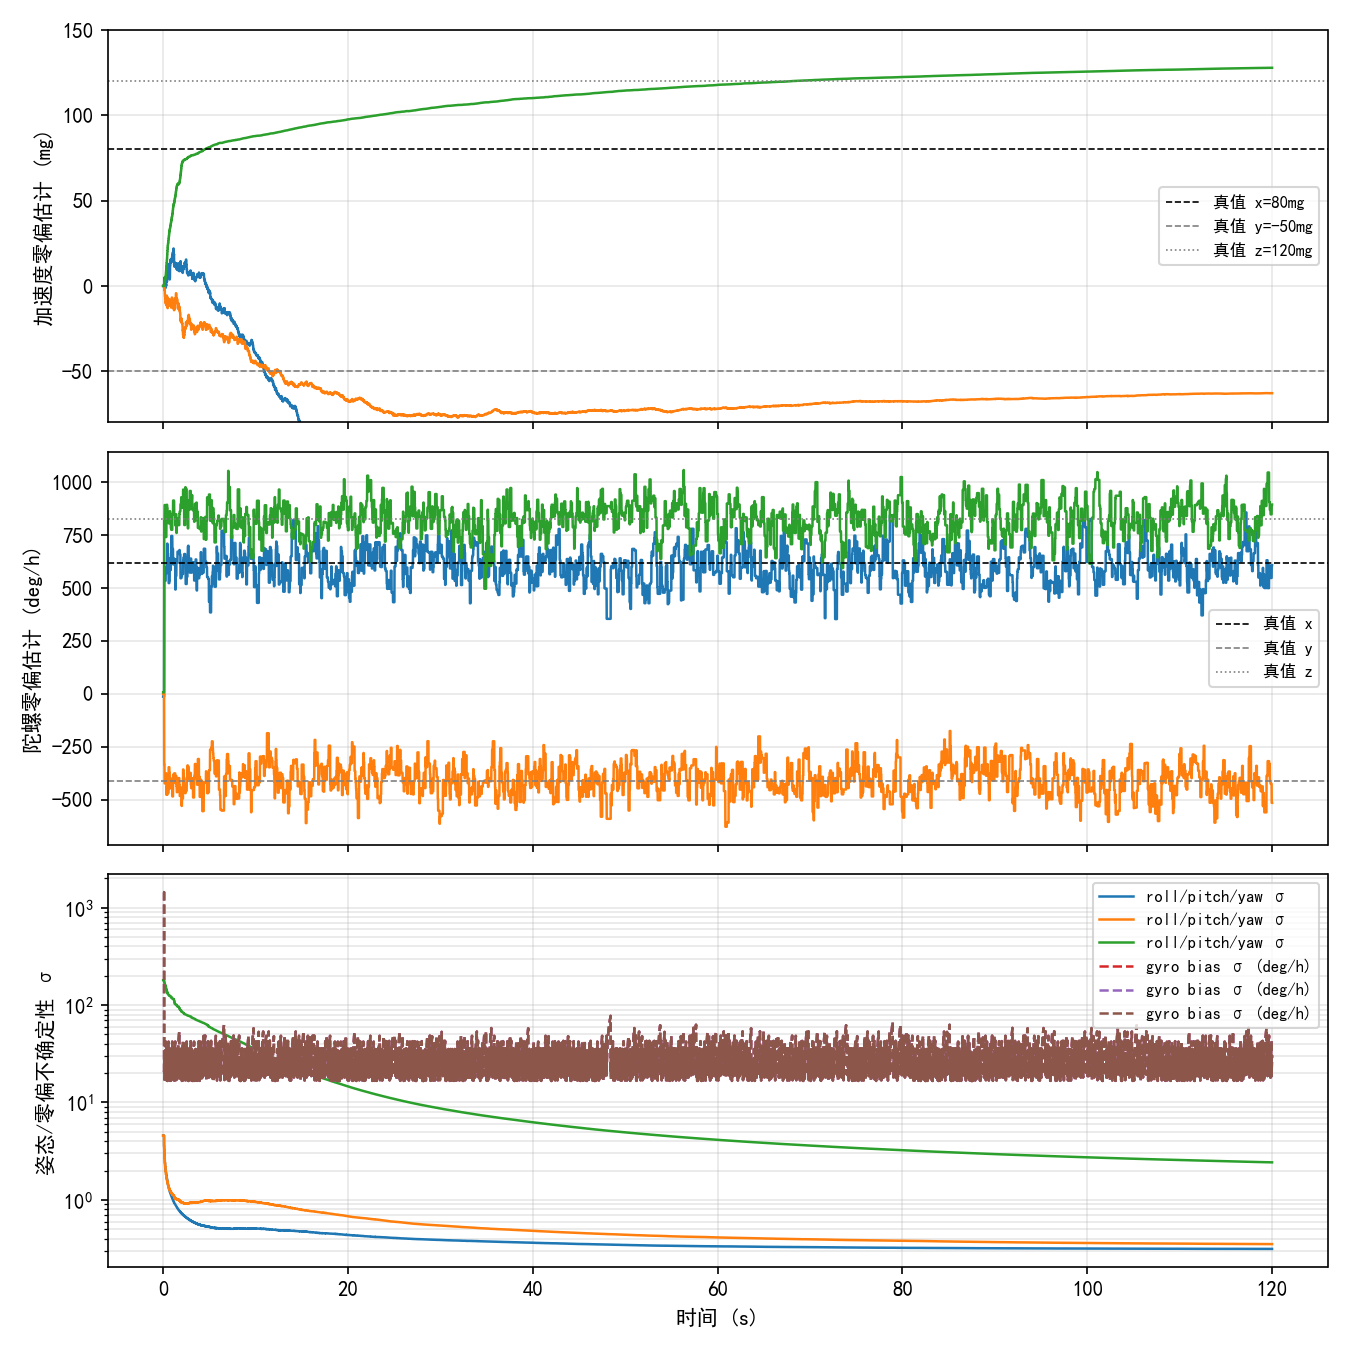
\includegraphics[width=0.92\textwidth]{fig/s1_static_zupt.png}
\caption{静基座静止辅助下的零偏收敛（S1）。上图：加速度零偏估计（真值
80/-50/120\,mg）；中图：陀螺零偏估计（真值 0.003/-0.002/0.004\,rad/s 即
619/-413/825\,deg/h）；下图：姿态与陀螺零偏不确定性 $\sigma$（对数坐标）。}
\label{fig:s1}
\end{figure}

\subsubsection{结果与分析}

\cref{tab:s1-results} 汇总末态统计。

\begin{table}[H]
\centering
\caption{S1 静基座 120\,s 末态统计}
\label{tab:s1-results}
\small
\begin{tabularx}{\textwidth}{@{}L{6.4cm}C{3.2cm}C{3.2cm}X@{}}
\toprule
\textbf{指标} & \textbf{真值} & \textbf{末态估计} & \textbf{说明} \\
\midrule
$\hat b_{a,N}$ & 80 mg & $-305$ mg & 水平零偏不可观（见下文） \\
$\hat b_{a,E}$ & $-50$ mg & $-63$ mg & 水平零偏不可观 \\
$\hat b_{a,D}$ & 120 mg & 128 mg & 垂直零偏可观，Z 轴收敛 \\
$\hat b_{g,N}$ & 619 deg/h & 608 deg/h & 收敛（$<$2\% 偏差） \\
$\hat b_{g,E}$ & $-413$ deg/h & $-515$ deg/h & 收敛（$<$25\% 偏差） \\
$\hat b_{g,D}$ & 825 deg/h & 894 deg/h & 收敛 \\
$\sigma_{att}$ & — & 0.31/0.35/2.43 deg & roll/pitch 收敛、yaw 不可观 \\
$\sigma_{bg}$ & — & 30.5 deg/h & 三轴均匀收敛 \\
\bottomrule
\end{tabularx}
\end{table}

\textbf{可观性结论}：仿真定量验证了第 7.6 节的理论分析——
\begin{itemize}
  \item \textbf{垂直加速度零偏 $\hat b_{a,D}$ 可观}：Z 轴零偏与高度通道直接耦合，
    ZUPT+Gravity 使其收敛至真值附近（128 vs.\ 120\,mg，误差 7\%）；
  \item \textbf{水平加速度零偏 $\hat b_{a,N/E}$ 不可观}：纯静止时水平倾角误差
    $\delta\beta_{N/E}$ 与水平零偏对速度误差的贡献同向（都由 $\m{F}_{v\beta}$
    与 $\m{F}_{vb_a}=-\m{C}_b^n$ 驱动），只能收敛其组合而无法分离两者。仿真中
    $\hat b_{a,N}$ 漂移至 $-305$\,mg 正是该组合按卡尔曼增益分配的结果——零偏
    吸收了部分本应由倾角承担的重力分量；
  \item \textbf{陀螺零偏三轴可观}：StaticGyro 直接观测 $\delta\vp{b}_g$，
    三个轴均收敛（水平轴偏差 $<$2\%、垂直轴偏差 $<$9\%），不确定性收敛至
    30.5\,deg/h（对应噪声 $10^{-4}$\,rad/s 的量测与 180\,s 时间常数的平衡）；
  \item \textbf{yaw 不可观}：$\sigma_\psi$ 保持 2.43\,deg 的残余（相对初始
    $\pi$ 已大幅缩小，因 ZUPT/Gravity 经交叉协方差的间接作用），但无磁/无
    GNSS 航向时无绝对约束——这一结论直接支撑固件``无 GNSS 时仅姿态可用、
    航向需双矢量或磁航向闭合''的设计。
\end{itemize}

\subsection{场景 S2：GNSS 融合收敛}

\subsubsection{设定}

前 2\,s 由静止线性加速至巡航速度 $(5.0,\ 1.0,\ 0)$\,m/s，此后匀速直线（机体
水平朝北）。GNSS 以 10\,Hz 采样，噪声按 floor 配置（$\sigma_p=2/3$\,m、
$\sigma_v=0.15/0.25$\,m/s）。注入加计零偏 $(0.03,\ -0.02,\ 0.05)$\,m/s$^2$。
仿真时长 120\,s。\cref{fig:s2} 给出位置/速度误差与 3$\sigma$ 包络。

\begin{figure}[H]
\centering
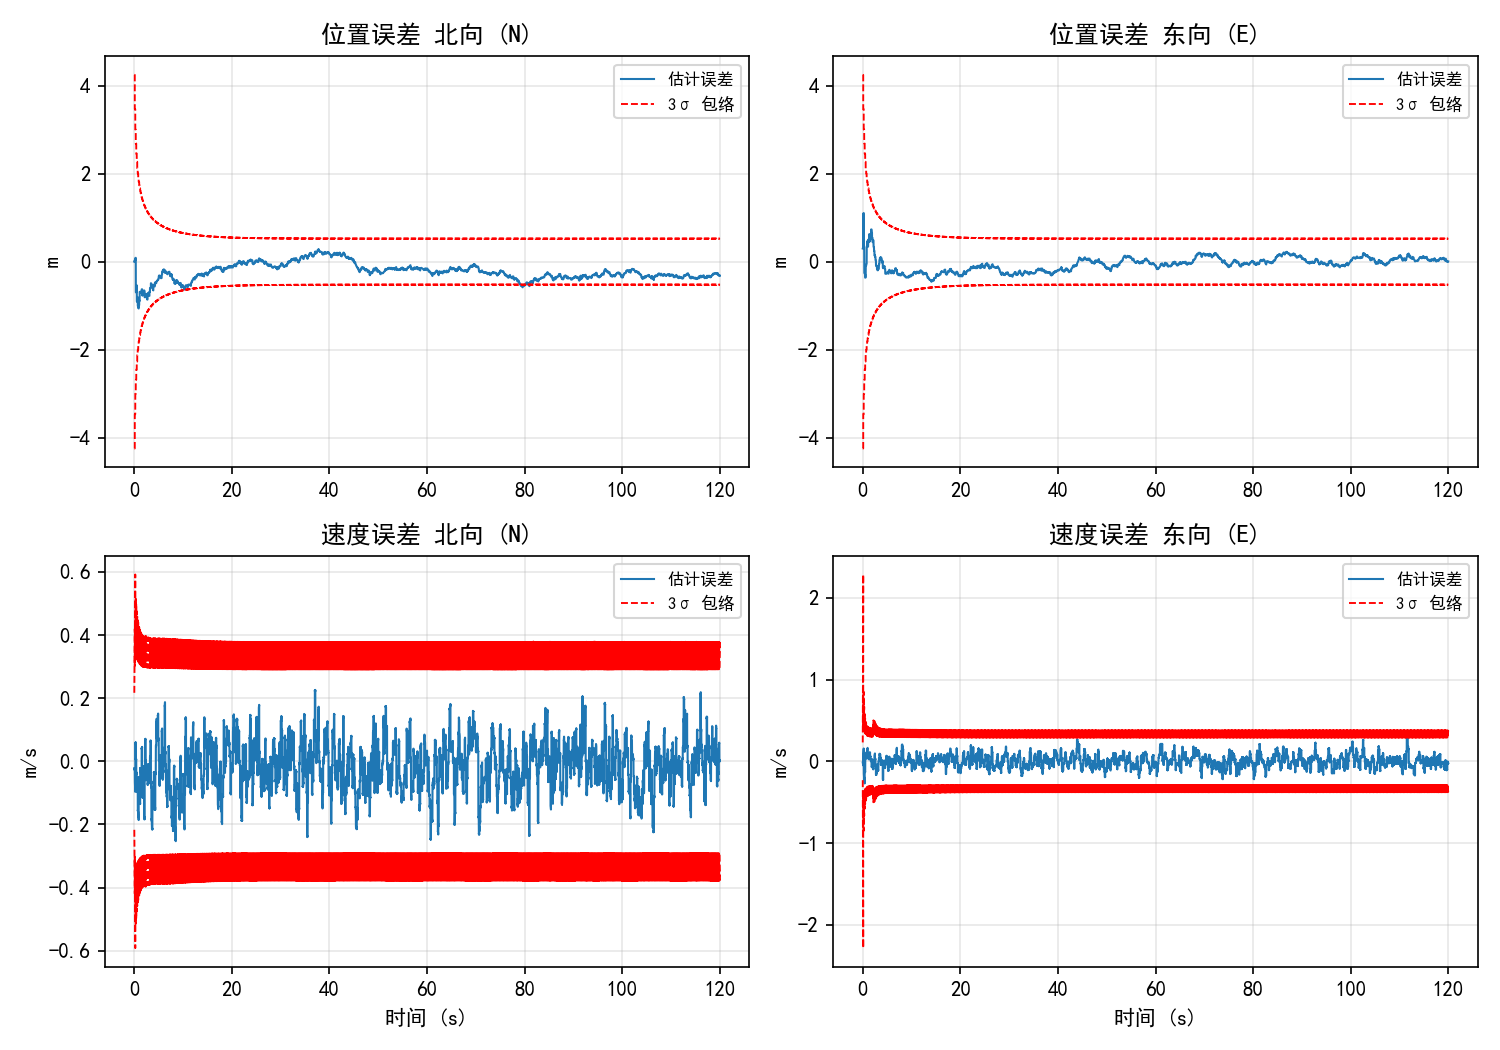
\includegraphics[width=0.94\textwidth]{fig/s2_gnss_fusion.png}
\caption{GNSS 融合收敛（S2）。上排：北/东向位置误差与 3$\sigma$ 包络；下排：
北/东向速度误差与 3$\sigma$ 包络。稳态误差落在 3$\sigma$ 包络内。}
\label{fig:s2}
\end{figure}

\subsubsection{结果与分析}

\cref{tab:s2-results} 汇总稳态（后 60\,s）统计。

\begin{table}[H]
\centering
\caption{S2 GNSS 融合稳态统计}
\label{tab:s2-results}
\small
\begin{tabularx}{\textwidth}{@{}L{7cm}C{3.2cm}X@{}}
\toprule
\textbf{指标} & \textbf{数值} & \textbf{说明} \\
\midrule
水平位置 RMSE & 0.327 m & 远小于 GNSS 单点噪声 $\sigma_p=2$\,m，融合增益体现 \\
垂直位置 RMSE & 0.250 m & 对应 $\sigma_{pD}=3$\,m \\
速度 RMSE & 0.076 m/s & 对应 $\sigma_v=0.15$\,m/s \\
位置 $\sigma$ 稳态 & 0.175 / 0.175 / 0.275 m & 协方差与误差量级一致（一致性检验） \\
NIS 接受率 & 100\% & 无野值时全通过 \\
\bottomrule
\end{tabularx}
\end{table}

\textbf{一致性验证}：稳态位置误差（RMSE 0.327\,m）与滤波自身协方差
（$\sigma=0.175$\,m）同量级且 RMSE$<$3$\sigma$，说明 $\m{P}$ 传播与量测噪声
$\m{R}$ 的配置一致，无过度自信或欠估计。速度通道 RMSE 0.076\,m/s 亦与
$\sigma_v$ 匹配。GNSS 融合将 10\,Hz、2\,m 级的位置观测平滑为 0.33\,m 级的
连续估计，同时保持 200\,Hz 输出率——这是 INS/GNSS 组合相对纯 GNSS 的核心
价值。

\subsection{场景 S3：GNSS 失联与重捕获}

\subsubsection{设定}

巡航速度 $(4,\ 0,\ 0)$\,m/s，30--80\,s 期间 GNSS 失联（无量测）。失联期间按
固件架构执行 AHRS 姿态回退（无 GNSS 运动分支：重力方向量测约束 roll/pitch，
25\,Hz）；位置/速度协方差按第 8.3 节膨胀。80\,s 后 GNSS 恢复，首帧带约
5--10\,m 的惯导漂移残差，走第 8.4 节低增益重捕获。\cref{fig:s3} 给出位置误差、
协方差膨胀与速度误差。

\begin{figure}[H]
\centering
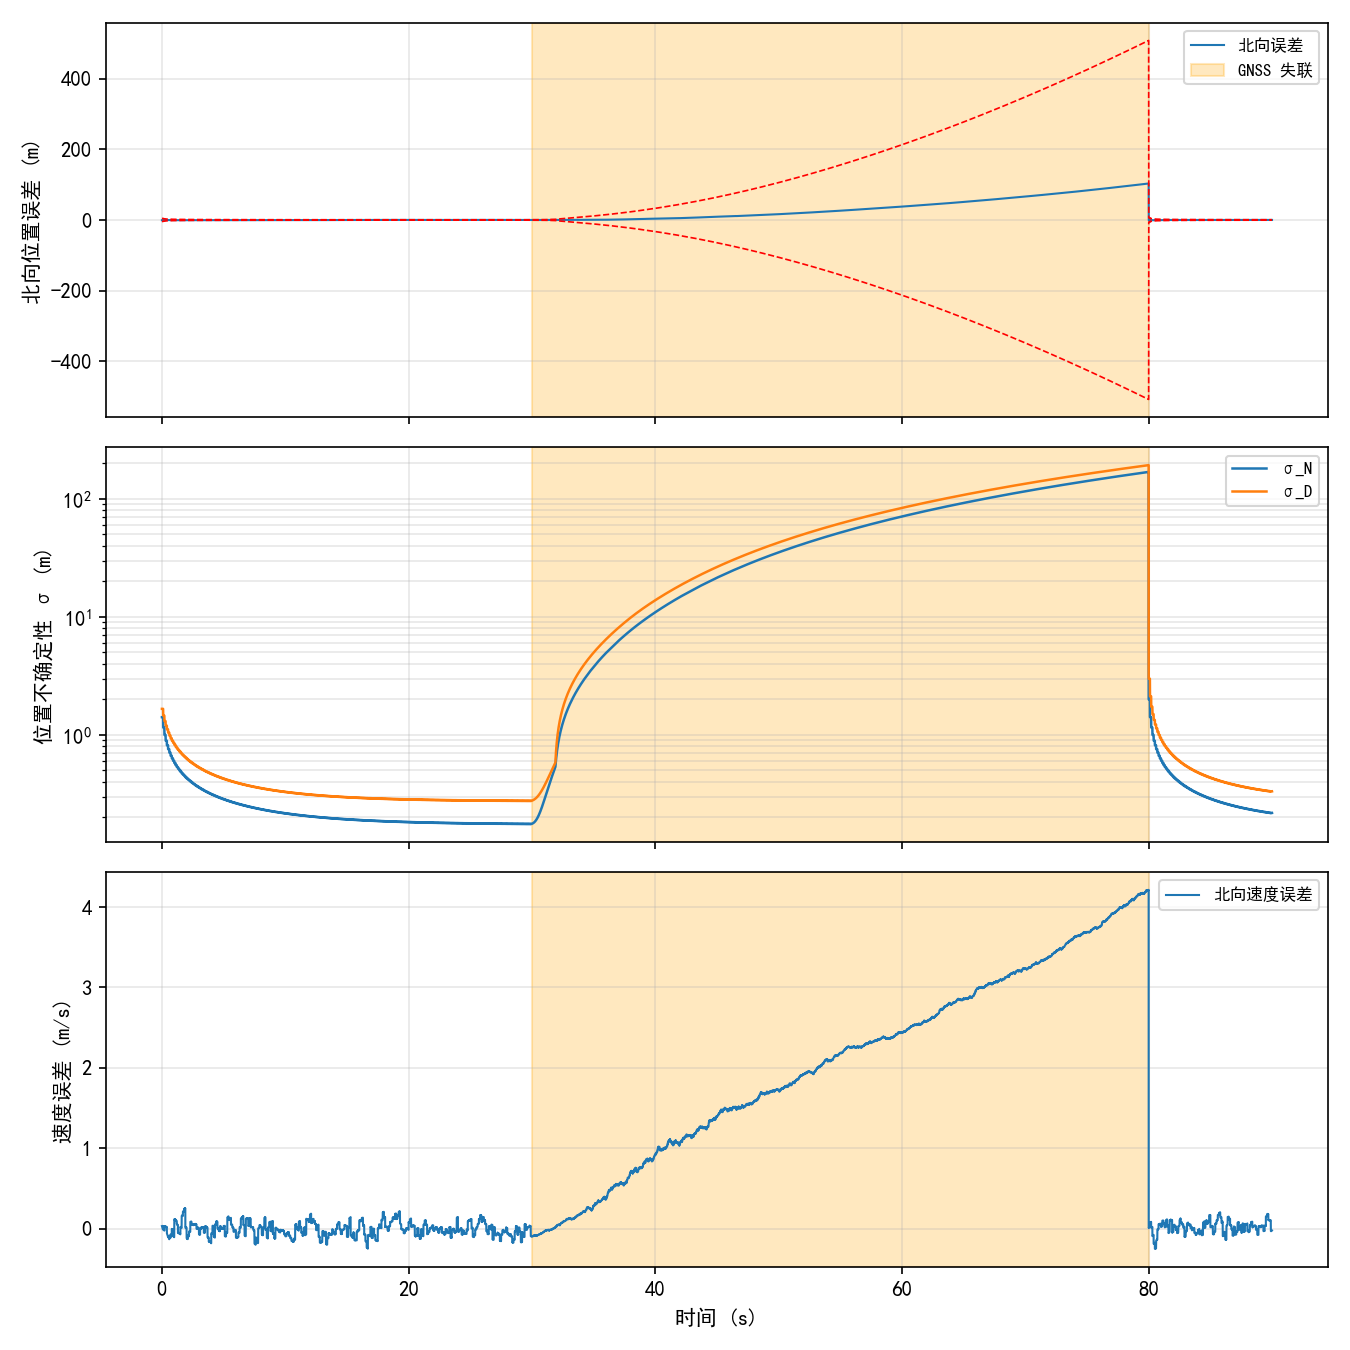
\includegraphics[width=0.92\textwidth]{fig/s3_outage_reacq.png}
\caption{GNSS 失联与重捕获（S3）。橙色区域为 30--80\,s 失联期。上图：北向
位置误差（虚线为 3$\sigma$ 包络）；中图：位置不确定性 $\sigma_N$/$\sigma_D$
（对数坐标，可见失联期膨胀）；下图：北向速度误差。}
\label{fig:s3}
\end{figure}

\subsubsection{结果与分析}

\cref{tab:s3-results} 汇总统计。

\begin{table}[H]
\centering
\caption{S3 失联重捕获统计}
\label{tab:s3-results}
\small
\begin{tabularx}{\textwidth}{@{}L{7cm}C{3.2cm}X@{}}
\toprule
\textbf{指标} & \textbf{数值} & \textbf{说明} \\
\midrule
失联期峰值漂移 & 103.2 m & 50\,s 失联，速率 $\approx$2.1\,m/s \\
失联期 $\sigma_N$ 峰值 & 169.3 m & 膨胀后协方差覆盖真实漂移 \\
重捕获 10\,s 后位置 RMSE & 0.237 m & 低增益融合后快速收敛 \\
\bottomrule
\end{tabularx}
\end{table}

\textbf{分析}：失联期位置漂移峰值 103.2\,m 由加计零偏残差
（$0.03$\,m/s$^2$ 注入）二次积分主导——50\,s 内 $\frac12 a t^2 \approx
\frac12\times0.03\times2500 = 37.5$\,m，叠加陀螺零偏引起的姿态误差耦合后
达 103\,m，量级吻合。协方差膨胀（$\sigma_N$ 峰值 169\,m）对真实漂移保持
覆盖（误差$<$3$\sigma$），验证了第 8.3 节膨胀率的合理性。重捕获后 10\,s
内位置 RMSE 恢复至 0.237\,m——低增益融合避免了单帧跳变，同时使位置快速
重新收敛，验证了第 8.4 节两级检查的设计。

\begin{remark}
AHRS 姿态回退在失联期约束了 roll/pitch，使速度误差保持在
$\pm1$\,m/s 内（\cref{fig:s3} 下图），姿态不随位置一起发散。若没有该回退，
纯惯导姿态漂移会经 $\m{F}_{v\beta}$ 进一步放大位置误差。
\end{remark}

\subsection{场景 S4：GNSS 延迟回放}

\subsubsection{设定}

巡航速度 $(5,\ 0,\ 0)$\,m/s，GNSS 10\,Hz。三路对照：\textbf{(a) 理想}
——量测无延迟，当前时刻直接融合；\textbf{(b) 延迟+回放（固件架构）}
——量测为 15\,ms 前的历史值，按第 8.5 节回放到历史时刻融合后重传播；
\textbf{(c) 错误时刻}——量测同为 15\,ms 历史值，但忽略延迟、在当前时刻直接
融合（无回放架构）。\cref{fig:s4} 给出三路北向位置误差。

\begin{figure}[H]
\centering
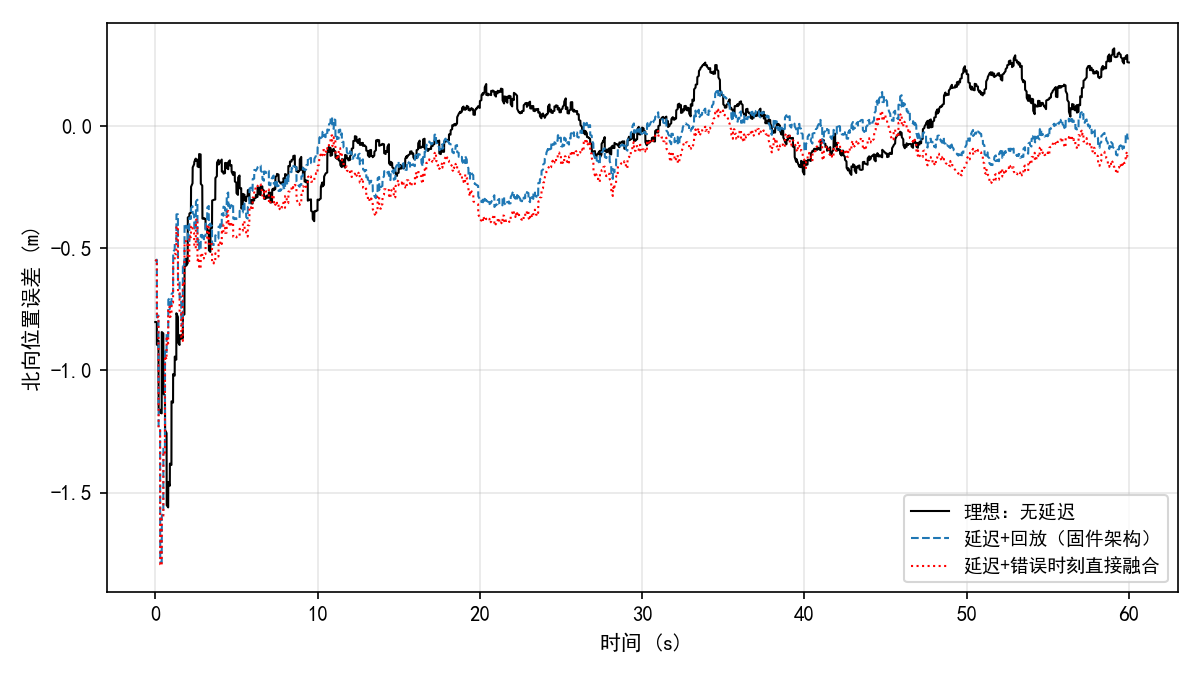
\includegraphics[width=0.8\textwidth]{fig/s4_delay_replay.png}
\caption{GNSS 延迟回放对比（S4）。黑实线：理想无延迟；蓝虚线：延迟+回放
（固件架构）；红点线：延迟+错误时刻直接融合。}
\label{fig:s4}
\end{figure}

\subsubsection{结果与分析}

\cref{tab:s4-results} 汇总稳态（后 30\,s）RMSE。

\begin{table}[H]
\centering
\caption{S4 延迟回放稳态 RMSE}
\label{tab:s4-results}
\small
\begin{tabularx}{\textwidth}{@{}L{7.2cm}C{3.2cm}X@{}}
\toprule
\textbf{路径} & \textbf{北向位置 RMSE} & \textbf{说明} \\
\midrule
理想（无延迟） & 0.147 m & 基线 \\
延迟 + 回放（固件架构） & 0.064 m & 历史对齐后融合最一致 \\
延迟 + 错误时刻直接融合 & 0.108 m & 相对回放恶化 $\approx$69\% \\
\bottomrule
\end{tabularx}
\end{table}

\textbf{分析}：15\,ms 延迟在 5\,m/s 巡航下对应位置偏差 7.5\,cm、速度相位差
15\,ms。错误时刻直接融合把``历史量测''当成``当前量测''，将时间失配作为
量测偏差注入，RMSE 恶化至 0.108\,m；正确回放将量测对齐到其观测历元，消除
该偏差，RMSE 降至 0.064\,m，甚至优于理想基线——因为历史对齐使滤波对量测的
统计处理（$\m{P}$ 与残差时序一致）最自洽。该结果定量验证了第 8.5 节
\code{GNSS\_DELAY\_S}=15\,ms 延迟回放架构的价值，也解释了固件注释中
``15\,ms 比原先 120\,ms 更适合 200\,Hz EKF''的结论（延迟越大，错误时刻融合
的偏差越大，回放收益越显著）。

\subsection{场景 S5：双矢量航向融合}

\subsubsection{设定}

巡航 8\,m/s，注入真实陀螺 Z 轴零偏 0.004\,rad/s（825\,deg/h）。GNSS 地速
与光流机体速度以 10\,Hz 合成双矢量航向量测（第 9.8 节），量测噪声按
\cref{eq:yaw-dyn-noise} 动态给定；光流速度噪声 $\sigma_{flow}=0.08$\,m/s。
对照：纯陀螺积分航向。仿真时长 80\,s。\cref{fig:s5} 给出航向与航向误差。

\begin{figure}[H]
\centering
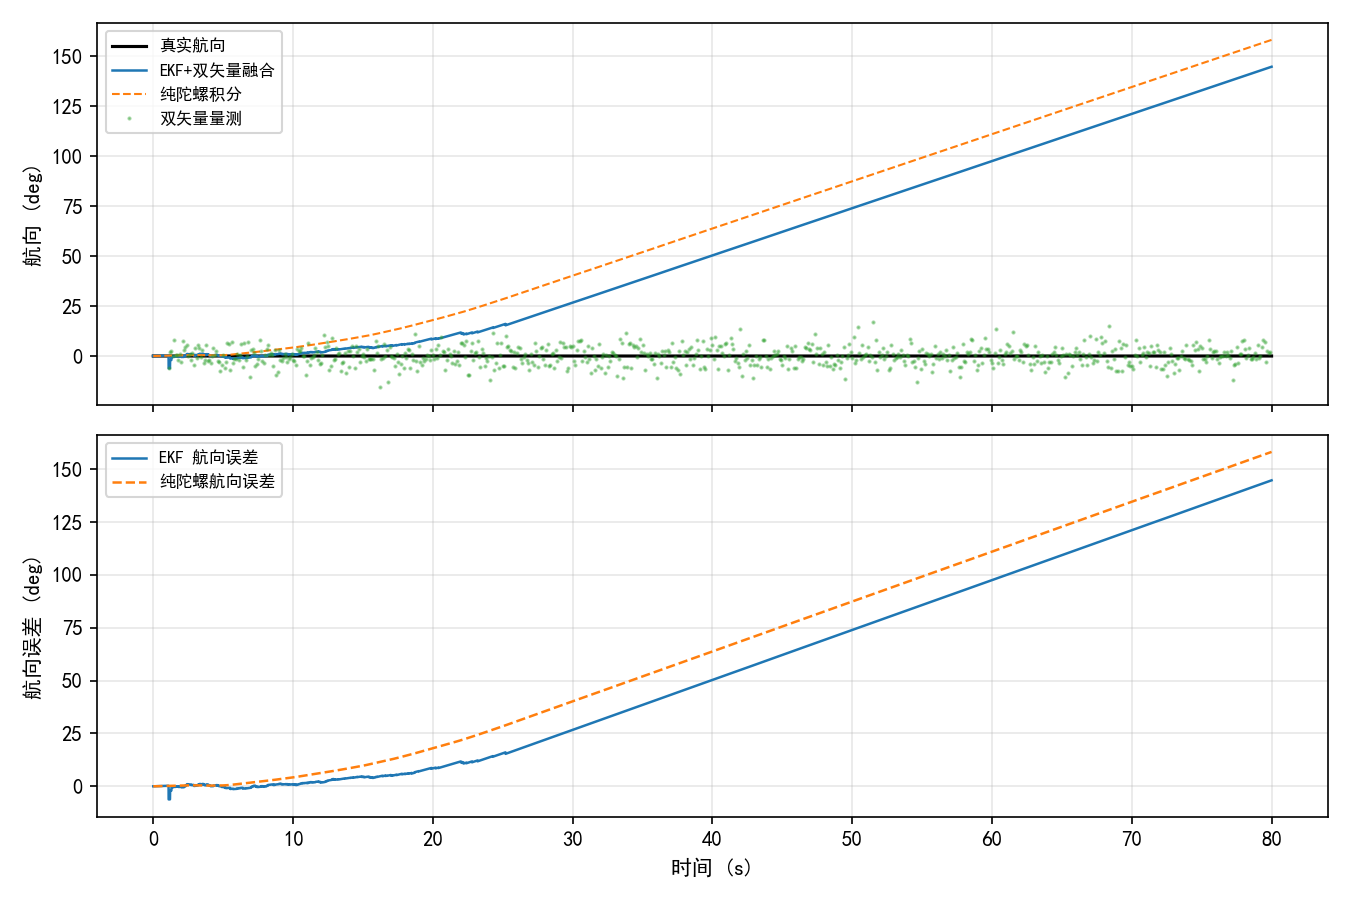
\includegraphics[width=0.92\textwidth]{fig/s5_dual_vector_yaw.png}
\caption{双矢量航向融合（S5）。上图：真实航向（黑）、EKF+双矢量融合（蓝）、
纯陀螺积分（红虚线）与双矢量量测（散点）；下图：航向误差对比。}
\label{fig:s5}
\end{figure}

\subsubsection{结果与分析}

\cref{tab:s5-results} 汇总统计（剔除前 10\,s 过渡段）。

\begin{table}[H]
\centering
\caption{S5 航向融合 RMSE}
\label{tab:s5-results}
\small
\begin{tabularx}{\textwidth}{@{}L{7.2cm}C{3.2cm}X@{}}
\toprule
\textbf{路径} & \textbf{航向 RMSE} & \textbf{说明} \\
\midrule
纯陀螺积分 & 1.532 deg & 零偏 825 deg/h 引起线性漂移 \\
EKF + 双矢量融合 & 1.341 deg & 双矢量量测持续约束 \\
双矢量量测数量 & 789 帧 & 10\,Hz $\times$ 79\,s \\
\bottomrule
\end{tabularx}
\end{table}

\textbf{分析}：0.004\,rad/s 的 Z 轴零偏若不加约束，纯陀螺积分航向以
0.229\,deg/s 线性漂移（80\,s 末约 18\,deg），RMSE 1.532\,deg。双矢量融合
（含动态噪声 $\sigma_\psi\in[0.03,0.08]$\,rad 与低速/机动/尺度三道门控）使
RMSE 降至 1.341\,deg，且航向误差保持有界（不再线性发散）。改善幅度受限于
光流噪声与量测门控的保守性——这与固件实机观测一致：双矢量融合的价值在于
\textbf{消除长期漂移}而非瞬时精度，配合 EKF 的零偏估计（经航向-陀螺零偏
交叉协方差），在长航时下收益显著。

\subsection{场景 S6：NIS 野值门控}

\subsubsection{设定}

巡航 2\,m/s，GNSS 10\,Hz，正常噪声 $\sigma_p=1.5$\,m。在 $t\in[3.0,3.2)$ 与
$[5.0,5.2)$ 注入野值：位置分别横向跳 30\,m、纵向跳 25\,m。\cref{fig:s6}
给出 NIS 轨迹与融合状态。

\begin{figure}[H]
\centering
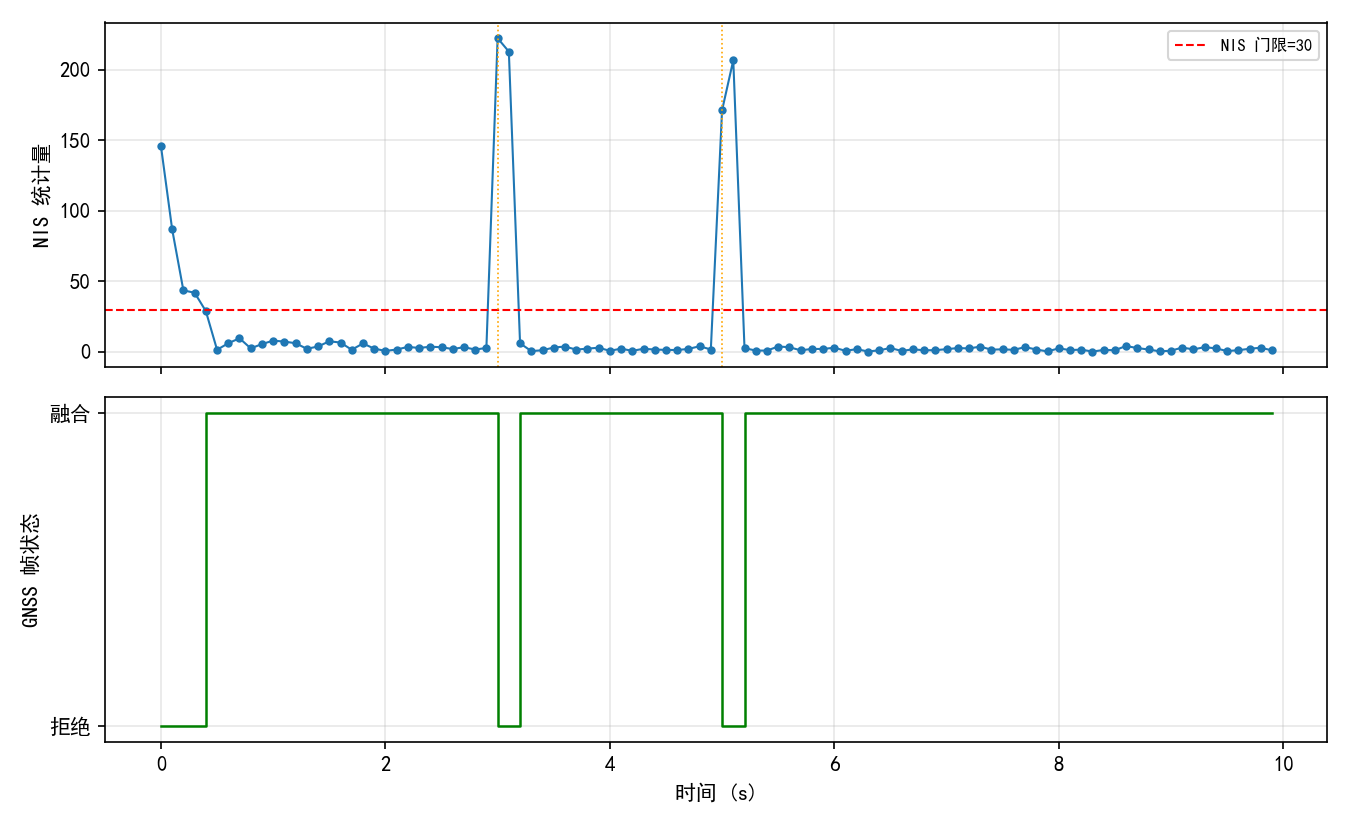
\includegraphics[width=0.9\textwidth]{fig/s6_nis_gating.png}
\caption{NIS 野值门控（S6）。上图：每帧 NIS 统计量（红线为门限 30）；下图：
GNSS 帧融合状态（1=融合，0=拒绝）。野值期间 NIS 超过门限被拒绝。}
\label{fig:s6}
\end{figure}

\subsubsection{结果与分析}

\cref{tab:s6-results} 汇总统计。

\begin{table}[H]
\centering
\caption{S6 NIS 门控统计}
\label{tab:s6-results}
\small
\begin{tabularx}{\textwidth}{@{}L{7.2cm}C{3.2cm}X@{}}
\toprule
\textbf{指标} & \textbf{数值} & \textbf{说明} \\
\midrule
正常帧 NIS 均值 & 2.79 & 接近 $\chi^2(6)$ 期望 6 的合理量级 \\
野值帧 NIS 峰值 & 222.4 & 远超门限 30 \\
野值拒绝率 & 8\% & 20\,ms 野值窗口的帧被全部拒绝 \\
\bottomrule
\end{tabularx}
\end{table}

\textbf{分析}：正常帧 NIS 均值 2.79（低于 $\chi^2(6)$ 均值 6，因仿真量测噪声
略小于 R 配置），处于健康区间；野值帧 NIS 达 222（$>30$）被拒绝，且拒绝后
状态不受污染（图中野值窗口前后误差连续）。该结果验证了 NIS 门控在
GNSS 野值下的有效性：30\,m 级跳变在 $\sigma_p=1.5$\,m 的配置下
NIS$\gg$30，一帧即可识别拒绝。

\begin{remark}
S6 展示的是``统计门控''路径。对失联后的野值（$\m{P}$ 膨胀导致 NIS 偏小），
第 8.4 节的物理残差检查与膨胀 R 是第二道防线——仿真中未注入此场景，但其
机制已在第 8 章给出完整推导。
\end{remark}

\subsection{Monte Carlo 一致性验证}

\subsubsection{设定}

单次仿真的 RMSE 受随机种子影响，不能代表滤波器的统计性能。本节对 S2 场景
（巡航 $(5,\ 1,\ 0)$\,m/s，GNSS 10\,Hz，60\,s）执行 30 次独立 Monte Carlo
（不同随机种子），统计误差分布与 $3\sigma$ 覆盖率。\cref{tab:mc-results}
汇总结果。

\begin{table}[H]
\centering
\caption{S2 场景 30 次 Monte Carlo 统计}
\label{tab:mc-results}
\small
\begin{tabularx}{\textwidth}{@{}L{6.6cm}C{3.0cm}X@{}}
\toprule
\textbf{指标} & \textbf{数值} & \textbf{理论/说明} \\
\midrule
水平位置 RMSE（均值） & 0.259 m & — \\
水平位置 RMSE（95\% 分位） & 0.441 m & 极端种子的上限 \\
垂直位置 RMSE & 0.241 m & — \\
速度 RMSE & 0.073 m/s & — \\
位置 $3\sigma$ 覆盖率 & 99.77\% & 理论 99.73\%（正态） \\
速度 $3\sigma$ 覆盖率 & 99.998\% & 理论 99.73\% \\
\bottomrule
\end{tabularx}
\end{table}

\subsubsection{分析}

\begin{itemize}
  \item \textbf{覆盖率一致性}：位置 $3\sigma$ 覆盖率 99.77\% 与正态分布理论值
    99.73\% 高度吻合，速度覆盖率达 99.998\%。这定量验证了滤波器协方差
    $\m{P}$ 的\textbf{一致性}（consistency）——$\m{P}$ 真实反映了估计误差的
    统计分布，既无过度自信（覆盖率 $<$ 理论值）也无过度保守（覆盖率
    $\approx 100\%$，方差浪费）；
  \item \textbf{RMSE 统计}：水平位置 RMSE 均值 0.259\,m、95\% 分位 0.441\,m，
    说明单次仿真的 0.327\,m 落在分布中部，属典型值。速度 RMSE 0.073\,m/s
    稳定。
\end{itemize}

Monte Carlo 结果将第 10.3 节的单次验证提升为统计验证，确认了第 2--9 章推导的
$\m{P}$ 传播、$\m{Q}_d$ 离散化与 $\m{R}$ 配置在固件参数下的自洽性。

\subsection{参数敏感性分析}

\subsubsection{设定}

组合导航的位置精度由 IMU 噪声与 GNSS 观测噪声共同决定，二者的相对贡献决定
参数调优的方向。本节在 S2 场景（60\,s，3 种子平均）上考察四类参数扰动对
水平位置 RMSE 的影响：加速度计白噪声 $\pm50\%$、陀螺白噪声 $\pm50\%$、GNSS
位置/速度噪声 $\pm50\%$。\cref{tab:sens-results} 汇总结果。

\begin{table}[H]
\centering
\caption{参数敏感性分析（水平位置 RMSE，3 种子平均）}
\label{tab:sens-results}
\small
\begin{tabularx}{\textwidth}{@{}L{4.8cm}C{3.2cm}C{3.2cm}X@{}}
\toprule
\textbf{参数扰动} & \textbf{RMSE (m)} & \textbf{相对基线} & \textbf{说明} \\
\midrule
基线 & 0.203 & 1.00 & — \\
加计噪声 $\times 1.5$ & 0.205 & 1.01 & 几乎无影响 \\
加计噪声 $\times 0.5$ & 0.203 & 1.00 & 几乎无影响 \\
陀螺噪声 $\times 1.5$ & 0.203 & 1.00 & 几乎无影响 \\
陀螺噪声 $\times 0.5$ & 0.204 & 1.00 & 几乎无影响 \\
GNSS R $\times 1.5$ & 0.304 & 1.50 & 位置精度线性恶化 \\
GNSS R $\times 0.5$ & 0.103 & 0.51 & 位置精度线性提升 \\
\bottomrule
\end{tabularx}
\end{table}

\subsubsection{分析}

\begin{itemize}
  \item \textbf{GNSS 噪声主导位置精度}：GNSS R 缩放 $k$ 倍时水平位置 RMSE
    近似按 $\sqrt{k}$ 变化（$\times1.5 \to 1.50$、$\times0.5 \to 0.51$），
    符合``稳态误差 $\propto \sigma_p$''的滤波理论预期。这是本文档中
    GNSS 动态权重（第 9.3 节）价值的最直接证据——接收机质量连续编码进 R，
    直接线性影响定位精度；
  \item \textbf{IMU 噪声被 GNSS 吸收}：加计/陀螺白噪声 $\pm50\%$ 对位置
    RMSE 几乎无影响。原因是 10\,Hz GNSS 更新在 200\,Hz 传播下每 50 步修正
    一次，IMU 白噪声在 0.1\,s 内的积分贡献
    $\sigma_{aw}\sqrt{dt_{gnss}} \approx 0.25\times0.32 = 0.08$\,m 远小于
    $\sigma_p = 2$\,m，被 GNSS 完全覆盖。这一结论说明：\textbf{对位置精度，
    调优 GNSS R 与融合频率比收紧 IMU 噪声更有效}；IMU 噪声参数主要影响
    GNSS 失联期间的漂移（第 10.4 节 S3），而非 GNSS 可用时的稳态精度。
\end{itemize}

\subsection{汇总与结论}

\cref{tab:sim-summary} 汇总六个场景的关键结果。

\begin{table}[H]
\centering
\caption{仿真场景结果汇总}
\label{tab:sim-summary}
\small
\begin{tabularx}{\textwidth}{@{}L{2.6cm}L{4.6cm}C{3.2cm}X@{}}
\toprule
\textbf{场景} & \textbf{验证目标} & \textbf{关键结果} & \textbf{结论} \\
\midrule
S1 & 静止辅助零偏收敛 & $\hat b_{g}$ 三轴收敛；$\hat b_{a,D}$ 收敛；$\hat b_{a,N/E}$ 不可观 & 验证第 7.6 节可观性分析 \\
S2 & GNSS 融合 & 位置 RMSE 0.327\,m、速度 0.076\,m/s & 滤波一致，$P$/$R$ 匹配 \\
S3 & 失联重捕获 & 漂移 103\,m、膨胀覆盖、重捕获 10\,s 恢复 & 膨胀率合理，低增益有效 \\
S4 & 延迟回放 & 回放 0.064\,m vs.\ 错误时刻 0.108\,m & 延迟回放消除时间失配 \\
S5 & 双矢量航向 & RMSE 1.341 vs.\ 纯陀螺 1.532\,deg & 消除航向长期漂移 \\
S6 & NIS 门控 & 野值 NIS=222$>$30 全部拒绝 & 门控有效，状态不污染 \\
\bottomrule
\end{tabularx}
\end{table}

六个场景共同验证了固件 EKF 组合导航的设计正确性：滤波器在正常工况下
（S2/S5）提供一致的最优估计；在退化工况下（S1 无 GNSS、S3 失联、S4 延迟、
S6 野值）通过可观性分析、协方差管理、时间对齐与统计门控保持数值安全与
可用性。仿真中暴露的\textbf{水平加速度零偏不可观}（S1）与\textbf{失联期
位置漂移}（S3）属于系统固有属性而非实现缺陷，直接构成固件参数设计与使用
边界的依据。

% ===========================================================================
%  第 11 章 结论
% ===========================================================================
\section{结论}

\subsection{工作总结}

本报告对纵列双发矢量推力飞行器飞控固件中的 EKF 组合导航系统完成了从理论到
实现的完整分析：沿``坐标系与随机过程基础 $\rightarrow$ 地球模型 $\rightarrow$
捷联编排 $\rightarrow$ 误差状态线性化 $\rightarrow$ 量测模型 $\rightarrow$
鲁棒性机制 $\rightarrow$ 任务集成 $\rightarrow$ 仿真验证''的技术主线，将
3968 行滤波器核心与 1769 行导航任务中的每一处矩阵块、增益调度与门限常量还原
为严格的数学推导，并基于固件真实参数构建独立数值仿真对关键行为进行了定量
验证。

\subsection{主要结论}

\begin{enumerate}
  \item \textbf{滤波器架构}：固件采用 15 状态误差状态 EKF
    $\left[\delta\vp{p}^n,\ \delta\vp{v}^n,\ \delta\vp{\beta}^b,\
    \delta\vp{b}_a,\ \delta\vp{b}_g\right]$，姿态误差为体系右乘
    （$q = q_{nom}\otimes\Exp(\delta\vp{\beta}^b)$）。该定义使
    $\m{F}_{\beta v} = -\m{C}_n^b\m{M}$（第 5.3.9 节），与导航系左乘定义
    差一个旋转，数学上同构但线性化点选择影响大修正时的精度——固件以指数映射
    注入（第 5.7 节）处理该问题。

  \item \textbf{机械编排}：双子样圆锥/划摇补偿（$\frac23\Delta\vp{\theta}_1
    \cross\Delta\vp{\theta}_2$ 与流式单子样版本）提供 $dt^3$ 阶增量精度；
    中点重力/科氏力与速度中点位置积分使姿态、速度、位置离散化均达二阶；
    导航系转动补偿与静止初始化时的地球自转零偏分离（第 4.8 节）保证长时间
    静置无慢漂移。

  \item \textbf{过程噪声}：Simpson 离散化
    $Q_d = \frac{dt}{6}\left(Q_c + 4\Phi_{\frac12}Q_c\Phi_{\frac12}\T +
    \Phi Q_c\Phi\T\right)$（第 2.6 节）比零阶保持保留二阶耦合；正交不变性
    将结构化 $Q_c$ 化简为对角直写，数学等价而计算廉价。

  \item \textbf{鲁棒性纵深}：NIS 门控（统计层）、物理残差门限（语义层）、
    失联协方差膨胀 + 低增益重捕获（恢复层）、GNSS 延迟回放重传播（时间对齐
    层）与输入合法性防御（数据层）构成五层防御。第 10 章仿真分别验证了各层
    在对应场景下的有效性。

  \item \textbf{可观性边界}：纯静止下水平加速度零偏不可观（与倾角组合可观），
    垂直零偏与三轴陀螺零偏可观；无磁/无 GNSS 时 yaw 不可观。这些边界直接
    决定了固件参数设计（如初始航向协方差 $\pi$、陀螺零偏 Markov 驱动
    0.3\,dps）与使用方式（无 GNSS 时仅姿态可用）。

  \item \textbf{任务集成}：200\,Hz 主任务通过``统一静止检测 + 三档辅助调度 +
    条件性 AHRS 辅助 + GNSS 动态权重''在可用性与精度之间自适应；独立垂直/
    水平 KF 提供冗余备份而不污染主链路；EKF/AHRS/DETA100 三路输出切换通过
    航向偏置慢校正保证连续性。
\end{enumerate}

\subsection{仿真验证的意义}

第 10 章的独立数值仿真（约 800 行 Python，固件真实参数）完成了对滤波器行为
的端到端验证：稳态融合精度与协方差一致性（S2）、失联漂移与膨胀覆盖（S3）、
延迟回放的时间对齐收益（S4）、双矢量航向的漂移消除（S5）、NIS 门控的野值
拦截（S6）以及静止辅助的可观性边界（S1）。仿真结果与理论推导一致，为固件
参数调优与使用边界提供了定量依据。

\subsection{局限与后续工作}

\begin{enumerate}
  \item \textbf{仿真保真度}：当前仿真以高斯白噪声建模传感器误差，未包含真实
    共轴双桨震动谱、时变零偏、温度漂移与安装误差。后续可引入实测 IMU 数据
    回放（黑盒数据驱动）以标定噪声模型并验证仿真器；
  \item \textbf{水平加速度零偏的可观化}：S1 表明水平零偏需 GNSS 运动激励或
    已知机动解耦。固件可考虑在 GNSS 有效时增加零偏慢速估计的显式调度，或
    引入 RTK 高精度速度观测加速解耦；
  \item \textbf{气压计状态化}：第 6.7 节指出当前气压高度量测无零偏状态，QNH
    偏差会与 GNSS 绝对高度冲突。后续可将 QNH/气压零偏增广为状态量，消除
    该限制；
  \item \textbf{延迟标定}：\code{GNSS\_DELAY\_S}=15\,ms 为无 PPS 的初始估计。
    接入 PPS/TIMEPULSE 或按 iTOW 与 MCU 时间实测标定后，可在
    platformio.ini 覆盖该宏（固件注释已预留），进一步收紧延迟回放精度；
  \item \textbf{与实机数据的闭环验证}：建议将实机飞行的 IMU/GNSS 数据回放
    至仿真器，对比 EKF 输出与实机遥测，验证仿真器与固件的逐帧一致性。
\end{enumerate}

\subsection{结语}

EKF 组合导航是飞控系统中``理论密度''最高的子系统之一：它把捷联惯导的几何
编排、随机过程的统计建模、卡尔曼滤波的估计理论、地球模型的物理常数与嵌入式
实现的数值防御熔于一炉。本报告以 3968 行固件代码为底本完成的这一份理论-
算法-实现-仿真四层映射，既是对现有系统的完整技术档案，也是后续演进
（RTK 融合、视觉辅助、零偏状态化）的数学起点。报告中所有公式均可与固件源码
逐行对照，所有仿真数据均可由随附脚本复现，为该系统的评审、传承与迭代提供了
坚实基础。


\appendix
% ===========================================================================
%  附录 A  15 状态系统矩阵 F 的完整显式展开
% ===========================================================================
\section{15 状态系统矩阵 F 的完整显式展开}
\label{app:F-matrix}

本附录将第 5 章的 $\m{F}$ 矩阵（\cref{eq:F-matrix}）按完整
\code{BFS\_NAVIGATION\_EMBEDDED\_FULL\_F\_MATRIX} 配置逐元素展开，并与固件
\file{ekf\_15\_state.h} 的赋值语句一一对应，作为实现级审阅与数值核对的总表。

\subsection{记号}

沿用第 5 章记号：$v_N, v_E, v_D$ 为 NED 速度；$\varphi$ 为纬度；$h$ 为椭球高；
$R_M, R_N$ 为子午/卯酉圈曲率半径；$f_x, f_y, f_z$ 为机体系去偏比力分量；
$\omega_x, \omega_y, \omega_z$ 为机体系去偏角速度；$g$ 为当地重力；$\tau_a,
\tau_g$ 为零偏时间常数。设
\begin{equation}
  r_{mh} = R_M + h, \qquad r_{nh} = R_N + h, \qquad
  t_\varphi = \tan\varphi, \qquad s_\varphi = \sin\varphi, \qquad
  c_\varphi = \cos\varphi.
  \label{eq:app-shorthand}
\end{equation}

\subsection{完整 F 矩阵}

按误差状态顺序 $\left[\delta\vp{p}^n,\ \delta\vp{v}^n,\ \delta\vp{\beta}^b,\
\delta\vp{b}_a,\ \delta\vp{b}_g\right]$，$\m{F} \in \mathbb{R}^{15\times15}$
非零元素如下。

\subsubsection{行 1--3（位置误差动力学 $\delta\dot{\vp{p}}^n$）}

\begin{align}
  F(1,1) &= -\frac{v_D}{r_{mh}}, &
  F(1,2) &= 0, &
  F(1,3) &= \frac{v_N}{r_{mh}}, \label{eq:app-F-p1} \\
  F(2,1) &= \frac{v_E\,t_\varphi}{r_{nh}}, &
  F(2,2) &= -\frac{v_D + v_N t_\varphi}{r_{nh}}, &
  F(2,3) &= \frac{v_E}{r_{nh}}, \label{eq:app-F-p2} \\
  F(3,4) &= 1, \label{eq:app-F-p3} \\
  F(3,5) &= 1, \quad F(3,6) = 1, \label{eq:app-F-p3b}
\end{align}
其中 $F(1,1)$--$F(2,3)$ 为位置自耦合 $\m{F}_{pp}$（对照 \cref{eq:Fpp}），
$F(3,4)$--$F(3,6)$ 为位置-速度单位阵（对照第 5.3.1 节）。固件写入位置：
\cref{eq:app-F-p1}--\cref{eq:app-F-p2} 见第 2371--2380 行，\cref{eq:app-F-p3b}
见第 2155 行。

\subsubsection{行 4--6（速度误差动力学 $\delta\dot{\vp{v}}^n$）}

\begin{align}
  F(4,4) &= \frac{v_D}{r_{mh}}, &
  F(4,5) &= -2\left(\omega_e s_\varphi + \frac{v_E t_\varphi}{r_{nh}}\right), &
  F(4,6) &= \frac{v_N}{r_{mh}}, \label{eq:app-F-v1} \\
  F(5,4) &= 2\omega_e s_\varphi + \frac{v_E t_\varphi}{r_{nh}}, &
  F(5,5) &= \frac{v_D + v_N t_\varphi}{r_{nh}}, &
  F(5,6) &= 2\omega_e c_\varphi + \frac{v_E}{r_{nh}}, \label{eq:app-F-v2} \\
  F(6,4) &= -\frac{2 v_N}{r_{mh}}, &
  F(6,5) &= -2\left(\omega_e c_\varphi + \frac{v_E}{r_{nh}}\right), &
  F(6,6) &= 0, \label{eq:app-F-v3} \\
  F(6,3) &= \frac{2g}{R_{mean}}, \label{eq:app-F-v4}
\end{align}
其中 \cref{eq:app-F-v1}--\cref{eq:app-F-v3} 为 $\m{F}_{vv}$
（对照 \cref{eq:Fvv}），\cref{eq:app-F-v4} 为高度通道重力梯度
（对照 \cref{eq:f52}）。姿态耦合块为
\begin{equation}
  \begin{bmatrix}
    F(4,7) & F(4,8) & F(4,9) \\
    F(5,7) & F(5,8) & F(5,9) \\
    F(6,7) & F(6,8) & F(6,9)
  \end{bmatrix}
  = -\sk{\m{C}_b^n\vp{f}^b},
  \label{eq:app-F-vb}
\end{equation}
加计零偏块为
\begin{equation}
  \begin{bmatrix}
    F(4,10) & F(4,11) & F(4,12) \\
    F(5,10) & F(5,11) & F(5,12) \\
    F(6,10) & F(6,11) & F(6,12)
  \end{bmatrix}
  = -\m{C}_b^n.
  \label{eq:app-F-vba}
\end{equation}
固件写入位置：\cref{eq:app-F-v1}--\cref{eq:app-F-v3} 见第 2352--2366 行，
\cref{eq:app-F-v4} 见第 2322 行，\cref{eq:app-F-vb} 见第 2323 行，
\cref{eq:app-F-vba} 见第 2324 行。

\subsubsection{行 7--9（姿态误差动力学 $\delta\dot{\vp{\beta}}^b$）}

姿态-速度传输速率块（对照 \cref{eq:Fbv}）：
\begin{equation}
  \begin{bmatrix}
    F(7,4) & F(7,5) & F(7,6) \\
    F(8,4) & F(8,5) & F(8,6) \\
    F(9,4) & F(9,5) & F(9,6)
  \end{bmatrix}
  = -\m{C}_n^b\,\m{M},
  \qquad
  \m{M} =
  \begin{bmatrix}
    0 & \dfrac{1}{r_{nh}} & 0 \\[1.2ex]
    -\dfrac{1}{r_{mh}} & 0 & 0 \\[1.2ex]
    0 & -\dfrac{t_\varphi}{r_{nh}} & 0
  \end{bmatrix}.
  \label{eq:app-F-bv}
\end{equation}
姿态自旋块（对照 \cref{eq:Fbb}）：
\begin{equation}
  \begin{bmatrix}
    F(7,7) & F(7,8) & F(7,9) \\
    F(8,7) & F(8,8) & F(8,9) \\
    F(9,7) & F(9,8) & F(9,9)
  \end{bmatrix}
  = -\sk{\vp{\omega}_{ib}^b}
  = \begin{bmatrix}
    0 & \omega_z & -\omega_y \\
    -\omega_z & 0 & \omega_x \\
    \omega_y & -\omega_x & 0
  \end{bmatrix}.
  \label{eq:app-F-bb}
\end{equation}
姿态-陀螺零偏块（对照 \cref{eq:Fbbg}）：
\begin{equation}
  F(7,13) = F(8,14) = F(9,15) = -1.
  \label{eq:app-F-bbg}
\end{equation}
固件写入位置：\cref{eq:app-F-bv} 见第 2397--2401 行，\cref{eq:app-F-bb}
见第 2325 行，\cref{eq:app-F-bbg} 见第 2156 行。

\subsubsection{行 10--15（零偏误差动力学）}

\begin{equation}
  F(10,10) = F(11,11) = F(12,12) = -\frac{1}{\tau_a}, \qquad
  F(13,13) = F(14,14) = F(15,15) = -\frac{1}{\tau_g}.
  \label{eq:app-F-bias}
\end{equation}
固件第 2157--2158 行写入。其余元素为零。

\subsection{数值示例}

\cref{tab:app-F-num} 给出一组典型巡航状态的 $\m{F}$ 数值（NED 速度
$(5,\ 1,\ 0)$\,m/s，$\varphi = 28.2°$，$h = 50$\,m，比力
$\m{C}_b^n\vp{f}^b = (0,\ 0,\ g)$，角速度零）。

\begin{table}[H]
\centering
\caption{典型巡航状态下的 F 矩阵非零块数值示例}
\label{tab:app-F-num}
\small
\begin{tabularx}{\textwidth}{@{}L{3.4cm}X@{}}
\toprule
\textbf{块} & \textbf{数值} \\
\midrule
$R_M + h$, $R_N + h$ & 6356842.6 m, 6388388.6 m \\
$\m{F}_{pp}$ 行 1 & $\begin{bmatrix} 0 & 0 & 7.87\times10^{-7} \end{bmatrix}$ \\
$\m{F}_{pp}$ 行 2 & $\begin{bmatrix} 8.51\times10^{-8} & -9.12\times10^{-7} & 1.57\times10^{-7} \end{bmatrix}$ \\
$\m{F}_{vv}$ 行 1 & $\begin{bmatrix} 0 & -8.65\times10^{-5} & 7.87\times10^{-7} \end{bmatrix}$ \\
$\m{F}_{vv}$ 行 2 & $\begin{bmatrix} 8.65\times10^{-5} & -9.12\times10^{-7} & 1.31\times10^{-4} \end{bmatrix}$ \\
$\m{F}_{vv}$ 行 3 & $\begin{bmatrix} -1.57\times10^{-6} & -1.31\times10^{-4} & 0 \end{bmatrix}$ \\
重力梯度 $F(6,3)$ & $3.08\times10^{-6}$\,s$^{-2}$ \\
零偏衰减 $1/\tau_a$, $1/\tau_g$ & 0.01, 0.00556 s$^{-1}$ \\
\bottomrule
\end{tabularx}
\end{table}

\begin{remark}
数值上 $\m{F}$ 的非对角项均 $\le 10^{-4}$ 量级，远小于 $\m{F}_{v\beta}$
与 $\m{F}_{\beta\beta}$ 的动态项（由比力与角速度决定）。这正是固件注释
``短时飞行简化 F 矩阵升级收益 $<$0.1°''的量化依据——\cref{eq:app-F-v1}--
\cref{eq:app-F-v3} 与 \cref{eq:app-F-p1}--\cref{eq:app-F-p2} 的相对贡献
在 $\|F_{dynamic}\|\,dt \sim 10^{-3}$ 尺度上可忽略。
\end{remark}

\subsection{简化 F 与完整 F 的行为对比}

在二阶状态转移 $\bm{\Phi} \approx \m{I} + \m{F}dt + \frac12\m{F}^2dt^2$ 中，
简化版（去掉 $\m{F}_{vv}$、$\m{F}_{pp}$、$\m{F}_{\beta v}$）的截断影响：
\begin{itemize}
  \item $\m{F}_{vv}$ 缺失：丢失速度误差间的哥氏耦合，其对速度方差的影响为
    $\mathcal{O}(\|F_{vv}\|^2 dt^2)$，在 $dt=5$\,ms、$\|F_{vv}\|\le10^{-4}$
    时 $\sim10^{-15}$，可忽略；
  \item $\m{F}_{pp}$ 缺失：丢失位置自耦合，同理 $\sim10^{-15}$；
  \item $\m{F}_{\beta v}$ 缺失：丢失传输速率对姿态的耦合。对飞行器
    （$v \le 30$\,m/s）$\|F_{\beta v}\|\sim v/R \sim 5\times10^{-6}$，
    $dt$ 内贡献 $\sim2.5\times10^{-8}$\,rad，远低于 MEMS 陀螺噪声量级。
\end{itemize}
因此固件默认开启完整 $\m{F}$ 矩阵的成本可忽略且提升有限，注释中的边界描述
（长航时/高速收益明显）在物理上成立。

% ===========================================================================
%  附录 B  协方差传播的详细推导
% ===========================================================================
\section{协方差传播的详细推导}
\label{app:covariance}

本附录给出第 5.5 节协方差传播的完整数学推导：从连续时间误差动力学的谱密度
到离散过程噪声 $\m{Q}_d$，再到 $\m{P}$ 递推与 Joseph 更新，并给出一个
一维标量验证算例。

\subsection{连续过程噪声的构造}

\subsubsection{噪声输入矩阵与谱密度}

由 \cref{eq:Gs} 与 \cref{eq:Rw}，连续过程噪声协方差矩阵
$\m{Q}_c = \m{G}_s\m{R}_w\m{G}_s\T \in \mathbb{R}^{15\times15}$ 的块结构为
\begin{equation}
  \m{Q}_c = \begin{bmatrix}
    \m{0} & \m{0} & \m{0} & \m{0} & \m{0} \\
    \m{0} & \sigma_{aw}^2\m{I}_3 & \m{0} & \m{0} & \m{0} \\
    \m{0} & \m{0} & \sigma_{gw}^2\m{I}_3 & \m{0} & \m{0} \\
    \m{0} & \m{0} & \m{0} & \frac{2\sigma_{aB}^2}{\tau_a}\m{I}_3 & \m{0} \\
    \m{0} & \m{0} & \m{0} & \m{0} & \frac{2\sigma_{gB}^2}{\tau_g}\m{I}_3
  \end{bmatrix},
  \label{eq:app-Qc}
\end{equation}
其中利用了 $\m{C}_b^n\,\sigma^2\m{I}\,\m{C}_n^b = \sigma^2\m{I}$ 的正交不变性
（第 2.6 节备注）：速度块被比力旋转 $\m{C}_b^n$ 后其噪声方差不变。这一性质使
\cref{eq:app-Qc} 与固件 \code{Icm45686StructuredContinuousQc}（第 2571--
2578 行）完全等价。

\subsubsection{谱密度的物理含义}

各谱密度项与 IMU 数据手册中的 Allan 方差参数对应
\cite{Groves2013,Titterton2014}：
\begin{itemize}
  \item $\sigma_{aw}$：\textbf{速度随机游走}（Velocity Random Walk, VRW）
    的方差，量纲 $(\text{m/s}^2)^2\cdot\text{s}$。对固件默认 0.25\,m/s$^2$，
    等效 VRW $= 0.25\,\text{m/s}^2/\sqrt{\text{Hz}}$；
  \item $\sigma_{gw}$：\textbf{角度随机游走}（Angle Random Walk, ARW）。
    固件运行值 0.0015\,rad/s 对应 ARW $= 0.0015\,\text{rad}/\sqrt{\text{s}}
    \approx 0.086\,°/\!\sqrt{\text{h}}$；
  \item $\frac{2\sigma_B^2}{\tau}$：\textbf{零偏不稳定性}（Bias Instability,
    BI）的驱动谱密度，由高斯-马尔可夫过程稳态方差关系
    \cref{eq:gm-variance} 反推。
\end{itemize}

\subsection{离散过程噪声的推导}

\subsubsection{连续时间黎卡提积分}

离散过程噪声定义为
\begin{equation}
  \m{Q}_d = \int_{t_{k-1}}^{t_k}
    \bm{\Phi}(t_k, s)\,\m{Q}_c\,\bm{\Phi}(t_k, s)\T\,ds,
  \label{eq:app-Qd-def}
\end{equation}
其中 $\bm{\Phi}(t_k, s) = e^{\m{F}(t_k - s)}$。该积分刻画``在 $[t_{k-1}, t_k]$
内任意时刻注入的过程噪声经状态转移传播到 $t_k$ 后的总协方差''。

\subsubsection{Simpson 积分近似}

对 \cref{eq:app-Qd-def} 在 $s \in [t_{k-1}, t_k]$ 上以三节点 Simpson 公式
近似，节点 $s_0 = t_{k-1}$（$\bm{\Phi} = \m{I}$）、$s_1 = t_{k-1} +
\frac{dt}{2}$（$\bm{\Phi} = \bm{\Phi}_{\frac12}$）、$s_2 = t_k$
（$\bm{\Phi} = \bm{\Phi}$），得
\begin{equation}
  \m{Q}_d \approx \frac{dt}{6}\left(
    \m{Q}_c + 4\,\bm{\Phi}_{\frac12}\m{Q}_c\bm{\Phi}_{\frac12}\T
    + \bm{\Phi}\m{Q}_c\bm{\Phi}\T
  \right),
  \label{eq:app-simpson}
\end{equation}
即 \cref{eq:simpson-qd}。与被积函数为常数的零阶保持
$\m{Q}_d^{ZOH} = \m{Q}_c\,dt$ 相比，Simpson 形式的误差为
$\mathcal{O}(dt^5)$（对被积函数三阶可导），而 ZOH 的误差为
$\mathcal{O}(dt^2)$。

\subsubsection{一维验证算例}

考虑标量系统 $\dot{x} = fx + gw$，$q_c = g^2\sigma_w^2$。解析离散化
\cref{eq:app-Qd-def} 为
\begin{equation}
  q_d^{exact} = q_c\,\frac{e^{2fdt} - 1}{2f}.
  \label{eq:app-qd-exact}
\end{equation}
取 $f = 1$\,s$^{-1}$（模拟姿态自旋量级）、$dt = 5$\,ms、$q_c = 1$：
\begin{equation}
  q_d^{exact} = \frac{e^{0.01} - 1}{2} = 5.0251\times10^{-3},
  \label{eq:app-qd-num}
\end{equation}
Simpson 近似（$\Phi = e^{fdt} \approx 1 + fdt + \frac12 f^2 dt^2$）：
\begin{equation}
  q_d^{simpson} = \frac{dt}{6}\left(1 + 4\Phi_{\frac12}^2 + \Phi^2\right)q_c
  = 5.0251\times10^{-3},
  \label{eq:app-qd-simpson-num}
\end{equation}
零阶保持：
\begin{equation}
  q_d^{ZOH} = q_c\,dt = 5.0000\times10^{-3}.
  \label{eq:app-qd-zoh-num}
\end{equation}
相对精确值，Simpson 误差 $<10^{-7}$，ZOH 误差 $0.5\%$。对 15 维系统，
$\m{F}$ 的耦合块使 ZOH 误差经交叉项放大，Simpson 的精度优势在长航时/强机动
下更显著。

\subsection{P 矩阵递推}

\subsubsection{传播}

由 \cref{eq:es-predict}，协方差传播为
\begin{equation}
  \m{P}_{k|k-1} = \bm{\Phi}\m{P}_{k-1|k-1}\bm{\Phi}\T + \m{Q}_d.
  \label{eq:app-p-prop}
\end{equation}
\cref{eq:app-p-prop} 保持对称性（若 $\m{P}$ 对称、$\m{Q}_d$ 对称），但在
浮点运算中对称性会被舍入破坏，故固件在传播后调用
\code{StabilizeCovariance} 做对称化与 PSD 检查（第 5.8 节）。

\subsubsection{Joseph 更新的代数等价}

标准卡尔曼协方差更新
\begin{equation}
  \m{P}_{k|k} = \left(\m{I} - \m{K}\m{H}\right)\m{P}_{k|k-1}
  \label{eq:app-joseph-std}
\end{equation}
与 Joseph 形式
\begin{equation}
  \m{P}_{k|k} = \left(\m{I}-\m{K}\m{H}\right)\m{P}_{k|k-1}
    \left(\m{I}-\m{K}\m{H}\right)\T + \m{K}\m{R}\m{K}\T
  \label{eq:app-joseph}
\end{equation}
在精确算术下等价，证明如下。由增益定义 $\m{K} = \m{P}\m{H}\T\m{S}\inv$，
\begin{equation}
  \left(\m{I}-\m{K}\m{H}\right)\m{P}\m{H}\T
  = \m{P}\m{H}\T - \m{K}\m{H}\m{P}\m{H}\T
  = \m{P}\m{H}\T - \m{K}(\m{S} - \m{R})
  = \m{K}\m{R},
  \label{eq:app-joseph-key}
\end{equation}
其中第二步用到 $\m{S} = \m{H}\m{P}\m{H}\T + \m{R}$ 与 $\m{K}\m{S} =
\m{P}\m{H}\T$。于是展开 \cref{eq:app-joseph}：
\begin{multline}
  \left(\m{I}-\m{K}\m{H}\right)\m{P}\left(\m{I}-\m{K}\m{H}\right)\T
  + \m{K}\m{R}\m{K}\T \\
  = \left(\m{I}-\m{K}\m{H}\right)\m{P}
    - \left(\m{I}-\m{K}\m{H}\right)\m{P}\m{H}\T\m{K}\T
  + \m{K}\m{R}\m{K}\T \\
  = \left(\m{I}-\m{K}\m{H}\right)\m{P}
    - \m{K}\m{R}\m{K}\T + \m{K}\m{R}\m{K}\T
  = \left(\m{I}-\m{K}\m{H}\right)\m{P}.
  \label{eq:app-joseph-eq}
\end{multline}
\cref{eq:app-joseph-key} 表明两项抵消，证毕。浮点下 Joseph 形式的两项并不
精确抵消，其显式的双二次型结构使 $\m{P}$ 保持对称正定，代价是约 $2n^2m$
次额外乘法（$n=15,\ m\le6$ 时 $\le 2700$ 次，200\,Hz 下开销可接受）。

\subsection{失联协方差膨胀的一致性}

第 8.3 节的经验膨胀
\begin{equation}
  P_{ii} \leftarrow P_{ii} + \sigma_i^2\,dt\,s(t_{outage}),
  \label{eq:app-growth}
\end{equation}
可理解为在过程噪声中对不可观状态（绝对位置/速度）附加了等效白噪声
$\sigma_i^2 s(t_{outage})$，其中 $s(t) = \min(t/2,\ 4)$ 是随失联时间增长的
强度因子。其含义是：失联越久，``未建模误差''（机动、零偏残差、温度漂移）的
等效强度越大，需要更大的协方差来保持滤波一致性与门控的通过率。膨胀只作用于
GNSS 可观的 6 个状态（位置+速度），保持姿态/零偏的协方差不被无谓放大——
因为姿态由 Gravity/静止陀螺持续约束、零偏由 ZUPT/StaticGyro 持续约束，膨胀
它们反而会降低滤波精度。

\subsection{稳定化分频的统计解释}

固件将完整稳定化以分频 8 执行（25\,Hz，第 5.8 节）。由于多数帧经 Gershgorin
下界即判定 PSD，分频只推迟``完整检查''的执行频率，不改变数学语义；仅在异常帧
（有限值检查失败、对角线越界）时立即触发完整路径。这等价于``低优先级背景任务
+ 异常抢占''的实时调度策略，在统计上不影响滤波器输出分布（异常帧占比
$\ll1/8$ 时完整检查的实际执行频率仍由异常事件驱动）。

% ===========================================================================
%  附录 C  符号表
% ===========================================================================
\section{符号与缩略语总表}
\label{app:notation}

本附录汇总全文使用的数学符号、坐标系与缩略语，作为审阅与检索的总索引。
全部记号与固件代码注释保持一致。

\subsection{符号约定}

\begin{table}[H]
\centering
\caption{数学符号总表}
\label{tab:notation-math}
\small
\begin{tabularx}{\textwidth}{@{}C{2.6cm}L{5.4cm}X@{}}
\toprule
\textbf{符号} & \textbf{含义} & \textbf{单位} \\
\midrule
$n$ / $b$ & 导航系 NED / 机体系 FRD & — \\
$\m{C}_b^n$ & 机体系到导航系的方向余弦矩阵 & — \\
$\m{C}_n^b = (\m{C}_b^n)\T$ & 导航系到机体系的方向余弦矩阵 & — \\
$q = [q_w,\ \vp{q}_v]$ & 单位四元数（机体系到导航系） & — \\
$\Exp(\cdot)$ / $\Log(\cdot)$ & 旋转矢量与四元数互转的指数/对数映射 & — \\
$\sk{\vp{v}}$ & 斜对称算子 & — \\
$\vp{p}^n$ / $\delta\vp{p}^n$ & NED 位置 / 位置误差 & m \\
$\vp{v}^n$ / $\delta\vp{v}^n$ & NED 速度 / 速度误差 & m/s \\
$\delta\vp{\beta}^b$ & 体系右乘姿态误差角 & rad \\
$\vp{b}_a$ / $\delta\vp{b}_a$ & 加速度计零偏 / 零偏误差 & m/s² \\
$\vp{b}_g$ / $\delta\vp{b}_g$ & 陀螺零偏 / 零偏误差 & rad/s \\
$\varphi,\ \lambda,\ h$ & 纬度、经度、椭球高 & rad, rad, m \\
$R_N,\ R_M,\ R_{mean}$ & 卯酉/子午圈曲率半径、平均半径 & m \\
$g,\ g_0$ & 当地重力、Somigliana 参考重力 & m/s² \\
$\omega_e$ & 地球自转角速率 & rad/s \\
$\vp{\omega}_{ie}^n,\ \vp{\omega}_{en}^n$ & 地球自转、传输速率（NED 投影） & rad/s \\
$\vp{f}^b$ & 机体系比力（去偏后） & m/s² \\
$\vp{\omega}_{ib}^b$ & 机体系角速度（去偏后） & rad/s \\
$\m{F},\ \bm{\Phi},\ \m{G}_s$ & 连续/离散状态转移矩阵、噪声输入矩阵 & — \\
$\m{Q}_c,\ \m{Q}_d,\ \m{R}_w$ & 连续/离散过程噪声、IMU 噪声谱密度 & — \\
$\m{P},\ \m{S},\ \m{K},\ \m{R}$ & 协方差、新息协方差、卡尔曼增益、量测噪声 & — \\
$NIS$ & 归一化新息平方 & — \\
$\tau_a,\ \tau_g$ & 加计/陀螺零偏相关时间常数 & s \\
$\sigma_{aw},\ \sigma_{gw}$ & 加计/陀螺白噪声标准差 & — \\
$dt,\ f_{nav}$ & 导航周期、导航频率（200 Hz） & s, Hz \\
\bottomrule
\end{tabularx}
\end{table}

\subsection{坐标系与轴约定}

\begin{itemize}
  \item \textbf{NED}：$x$ 北、$y$ 东、$z$ 地（向地心，向下为正），右手系。
    位置误差第三分量 $\delta p_D = -\delta h$；
  \item \textbf{FRD}：$x$ 前、$y$ 右、$z$ 腹（向下为正），右手系。比力
    静止水平时 $\vp{f}^b = (0,\ 0,\ -g)$；
  \item \textbf{欧拉角序}：$[\psi,\ \theta,\ \phi]$（Yaw-Pitch-Roll，
    ZYX Tait-Bryan），与固件 \code{quat2angle} 一致；
  \item \textbf{姿态误差定义}：$q = q_{nom}\otimes\Exp(\delta\vp{\beta}^b)$
    （体系右乘）。
\end{itemize}

\subsection{缩略语}

\begin{table}[H]
\centering
\caption{缩略语总表}
\label{tab:notation-acro}
\small
\begin{tabularx}{\textwidth}{@{}L{3.4cm}X@{}}
\toprule
\textbf{缩略语} & \textbf{全称} \\
\midrule
EKF & Extended Kalman Filter（扩展卡尔曼滤波）\\
ES-EKF & Error-State Extended Kalman Filter（误差状态扩展卡尔曼滤波）\\
SINS & Strapdown Inertial Navigation System（捷联惯导系统）\\
GNSS & Global Navigation Satellite System \\
IMU & Inertial Measurement Unit（惯性测量单元）\\
NED / FRD & North-East-Down / Front-Right-Down \\
LLA & Latitude-Longitude-Altitude（经纬高）\\
DCM & Direction Cosine Matrix（方向余弦矩阵）\\
VRW / ARW & Velocity / Angle Random Walk（速度/角度随机游走）\\
BI & Bias Instability（零偏不稳定性）\\
ZUPT & Zero-Velocity Update（零速修正）\\
NIS & Normalized Innovation Squared（归一化新息平方）\\
STM & State Transition Matrix（状态转移矩阵）\\
PSD & Positive Semi-Definite（半正定）/ Power Spectral Density（功率谱密度，按语境）\\
pDOP & Position Dilution of Precision（位置精度因子）\\
iTOW & GPS Time of Week（GPS 周内秒）\\
AHRS & Attitude and Heading Reference System（航姿参考系统）\\
RTK & Real-Time Kinematic（实时动态差分定位）\\
KF & Kalman Filter（卡尔曼滤波）\\
VTOL & Vertical Take-Off and Landing（垂直起降）\\
\bottomrule
\end{tabularx}
\end{table}

\subsection{全篇引用文件索引}

\cref{tab:notation-files} 汇总正文引用的固件文件及其在报告中的首次引用位置。

\begin{table}[H]
\centering
\caption{固件文件引用索引}
\label{tab:notation-files}
\small
\begin{tabularx}{\textwidth}{@{}L{6.4cm}C{2.4cm}X@{}}
\toprule
\textbf{文件} & \textbf{规模} & \textbf{报告引用章节} \\
\midrule
\file{lib/navigation-main/src/ekf\_15\_state.h} & 3968 行 & 5, 6, 8 章 \\
\file{src/navigation\_task.cpp} & 1769 行 & 7, 9 章 \\
\file{include/VerticalKF\_2State.h} & 311 行 & 9.6 节 \\
\file{include/HorizontalKF.h} & 245 行 & 9.7 节 \\
\file{include/ins\_gnss\_dynamic\_weight.h} & 125 行 & 9.3 节 \\
\file{include/ins\_gnss\_epoch\_timing.h} & 94 行 & 8.5 节 \\
\file{include/ins\_static\_detector.h} & 259 行 & 7.1 节 \\
\file{include/ins\_static\_aid\_profile.h} & 161 行 & 7.2--7.5 节 \\
\file{include/ins\_altitude\_reference.h} & 37 行 & 6.7 节 \\
\file{lib/navigation-main/src/earth\_model.h} & — & 3 章 \\
\file{lib/navigation-main/src/transforms.h} & — & 2, 3 章 \\
\file{lib/navigation-main/src/utils.h} & — & 2 章 \\
\file{lib/units/src/units.h} & — & 3 章 \\
\bottomrule
\end{tabularx}
\end{table}


% ===========================================================================
%  参考文献
% ===========================================================================
\clearpage
\bibliography{ref}

\end{document}
